\part{Manure Module}
% Global Table of Contents
\thispagestyle{fancy}

% Local TOC that includes only what’s inside THIS section
\etocsettocstyle{\subsection*{Contents}}{} % heading for the local toc
\etocsetnexttocdepth{subsection}           % or subsubsection
\localtableofcontents
\newpage

\section*{List of Figures}
\locallistoffigures
\newpage

\section*{List of Tables}
\locallistoftables
\newpage


\section{Module Introduction}
\begin{refsection}
\par\noindent\justifying
The responsibility of the manure module in RuFaS is to simulate the loss and/or gain of manure mass and nutrients on a daily timestep at each step of the manure management chain on a dairy farm. On the majority of farms, manure represents an important link in the cycling of nutrients through animals, land, crops, and back to animals. Therefore, modeling both greenhouse gas (GHG) emissions as well as non-GHG nutrient and losses is crucial in capturing nutrient flows through the whole-farm system. 
    
The manure module accomplishes its responsibilities by tracking a critical, core set of variables called “ManureStream” variables, which include key agronomic nutrients (N, P, K), carbon (e.g. total and volatile solids), water, ash, mass, and volume. The Manure Module receives manure excretion and bedding information from the animal module, then passes manure through the manure management chain, until manure is either applied to fields or exported. The specific steps of the manure management chain are user-defined, and the individual steps/options in manure management chains are referred to as “processors”. The exact chemical, physical, or other processes that occur at each step along the management chain depend on what type of processor the manure is being held in. For example, parlor cleaning processors, which represent removing manure from the milking parlor and holding areas, principally add water to manure but do not estimate GH emissions or other nutrient losses. A slurry storage outdoor processor (a type of manure storage), however, estimates daily methane (CH\textsubscript{4}) and ammonia (NH\textsubscript{3}-N) losses, which are then reflected by reducing the quantity of nutrients remaining in the stored manure at the end of the day. 


\subsection{Structural setup of the Manure Module}
    Processors in the Manure Module fall into four basic classes, with multiple types available within each class. The processor classes are intended to represent the common, primary steps in manure management. They include manure handling (which refers to the daily activities of cleaning and removing manure from facilities or managing it in place), storage, and manure treatment, such as anaerobic digestion or mechanical solid liquid separation. 

\begin{table}[h!]
\centering
\renewcommand{\arraystretch}{1.3}
\caption{Examples of processor types by class.}
\begin{tabular}{@{} L{3cm} L{10cm} @{}}
\toprule
\multicolumn{1}{c}{\textbf{Classes}} & 
\multicolumn{1}{c}{\textbf{Types}} \\
\midrule

\textbf{Handler} & Manual Scraping; Alley Scraper; Flush System; Parlor Cleaning \\
\textbf{Digester} & Continuous Mix \\
\textbf{Separator} & Screw Press; Rotary Screen \\
\textbf{Storage} & Composting; Open Lot; Bedded Pack; Slurry Storage Outdoor; Slurry Storage Underfloor; Anaerobic Lagoon \\

\bottomrule
\end{tabular}
\end{table}

 


\vspace{0.5cm}

How manure moves between processors is based on defining the destination processor that any one processor should send its manure to, and the proportion(s) of manure from the originating processor that should go there. For example, if 50\% of manure from a single pen is routed to storage A, and 50\% to storage B, the manure handler processor assigned to that pen will have two destinations defined (storage A and storage B), with the proportion going to each defined as 0.50. By controlling destinations and proportions, the user is able to define aggregating (i.e., assigning manure from two separate processors to the same destination) and splitting (assigning manure from one processor to two or more locations) behavior. A visual example is below and illustrates the manure management chain without RuFaS-specific syntax. The next figure illustrates RuFaS-specific information (e.g. specific processor names, creation of manure streams in the animal module, etc.). Note that the splitting of manure generated from singular pens in the Animal Module illustrated in Figure 8 is covered in the Animal to Manure Connection document. 


    \begin{figure}[H] % The 'p' option places the figure on a page by itself
    \centering
    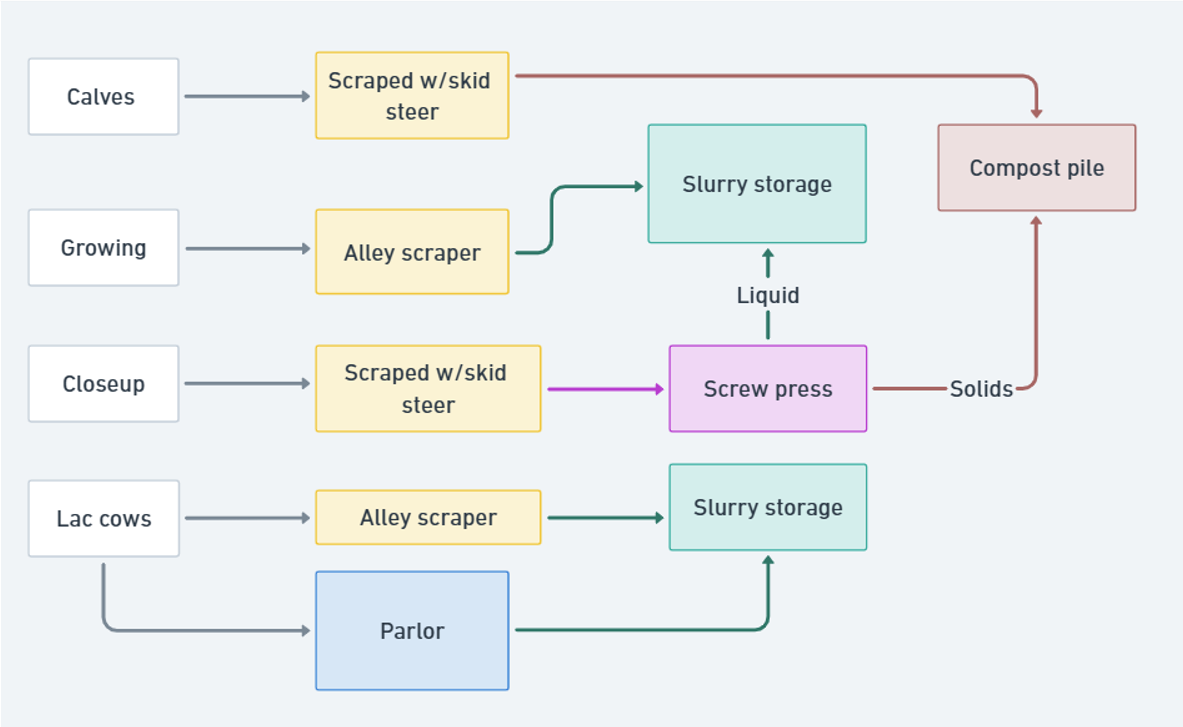
\includegraphics[width=0.9\textwidth]{resources/manuremanchain.png} % Replace with your image file
    \caption{A real-world example of a simplistic manure management chain.  }
       \end{figure}




    \begin{figure}[H] % The 'p' option places the figure on a page by itself
    \centering
    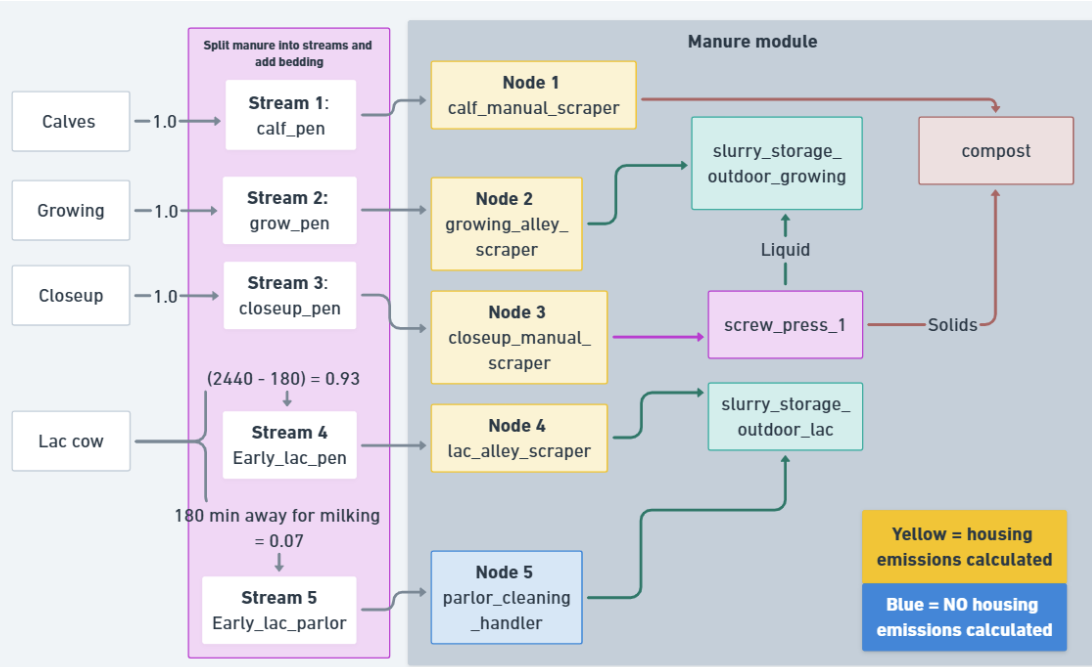
\includegraphics[width=0.9\textwidth]{resources/overviewmanure.png} % Replace with your image file
    \caption{The manure management chain illustrated in the previous figure, with RuFaS-specific information reflected. }

    \end{figure}


\subsection{Overview of Required Inputs}
There are two general categories of input required from the user: 
	\begin{enumerate}
            \item Which processors are used and how do they work (processor-specific configurations) E.g., storage time length, use of a cover 
            \item Destination and proportion(s) allocated to destination(s) of manure passed from each processor 
	\end{enumerate}


Information on inputs required and options available for each individual processor are outlined in the individual processor documentation. 
\vspace{0.2cm}

For defining destinations and proportions, there are very few rules and restrictions on how manure can be moved between processors. The primary rule for defining processor destinations is that users cannot define loops, i.e., manure from a processor “downstream” in a manure management chain cannot return its manure to a processor “upstream”.
\vspace{0.2cm}

\begin{tcolorbox}[colback=white, colframe=black, boxrule=0.5pt, arc=3pt, width=\textwidth]
The assignment of manure generated in the Animal Module (which also reflects the quantity of bedding used) to its destination in the Manure Module occurs in the Animal Module. See the Animal to Manure Connection section for more information. 

\end{tcolorbox}
\vspace{0.2cm}

\subsection{General Assumptions of the Manure Module}
        \begin{enumerate}
            \item All manure is recovered unless otherwise specifically stated. For example, all manure excreted by animals is assumed to be captured by manure handlers, all manure in a manure storage is assumed to be completely removed when the storage is emptied (unless explicitly noted in the specific processor’s documentation), etc. 
            \item Manure moves through the manure management chain once, and only once, per day. With this, values are reported on a daily timestep, and represent the current state at the end of the given day (e.g. CH\textsubscript{4} emissions from this day, amount of N left in storage on this day, etc.). 
                \begin {itemize}
                    \item Storage processors include a user-defined “storage time”, during which manure accumulates in the storage until reaching the end of the time interval, at which point it is passed to the next processor or exported, if the storage comes last in the manure chain.  The minimum storage time value is 1, thus manure cannot move through more than one storage per day. 
                    \item For processors without a storage time option, manure is assumed to move through the processor immediately. E.g., on a single day, excreted manure may move through a handler, continuous mix digester, separator, and into composting storage, with each processor reporting the quantity and composition of manure they either passed to the next processor or are holding in storage.
                \end{itemize}
            \item The Manure Module adheres to the principle of mass balance, meaning, the quantity of manure nutrients remaining in manure is proportional to the quantity of the nutrient lost through biological or physical processes. The same is true for additions of mass/nutrients.
                \begin{itemize}
                    \item One current exception to this is N loss. N losses are not currently reflected in the total mass of manure; this exception will be addressed and corrected in the near future. 
		      \end{itemize}
        \end{enumerate}

\textbf{Manure Storage Assumptions}
	\begin{enumerate}
            \item Received manure nutrients entering a storage are added to accumulated mass/nutrient quantities prior to calculating gas emissions each day.
            \item When the end of the storage’s user defined storage time is reached, the accumulated manure in storage is removed completely and entirely, and is passed to the next processor in the chain (e.g., a subsequent storage, field application, etc.).
            \item Emptying intervals (in days) are defined by the user in equal lengths at this time, e.g., manure storage can be emptied every 3 months (e.g. in April, July, October, January) but cannot be emptied in April, then 2 months later in June, and then 3 months later in September. However, timing of storage emptying (e.g. April and October emptying vs. May and November emptying) can be set according to the general simulation dates to simulate more realistic manure removal behavior.
	\end {enumerate}


\section{Animal and Manure Module Connection} 
\subsection{Introduction}

    Though animals are typically fed and managed in groups, referred to as pens in RuFaS, manure from a single group of animals may not always remain in or be transported to the same location on the farm. For example, lactating cows who must travel to a milking parlor deposit some proportion of their manure outside of their pen. Or, in open lot systems, manure deposited in the concrete feed alley apron is often removed and managed separately from manure deposited on the lot surface. Additionally, more than one type of bedding may be used in a pen (e.g., no bedding during summer but straw provided in winter), which also eventually becomes part of manure. Considering this, RuFaS accommodates routing of manure from a single group (pen) of animals to multiple locations, which are then received by the Manure module. This document describes how a pen’s total manure excretion and bedding are allocated to one or more discrete quantities of manure, referred to as manure streams, and passed to the Manure module. How the user configures this manure routing and bedding options and addition of bedding to manure are also described here.

    \vspace{0.25cm}
    \textbf{Implementation in RuFaS} 
    \vspace{0.25cm}

    The Animal module is responsible for calculating manure excretion mass and composition based on animal attributes, ration composition and intake, and other factors. The Animal module must then pass this manure on to the Manure module, where manure nutrient gains and losses are quantified through field application or export. The Animal module currently calculates manure excretion at the pen level (i.e., values representative of the total manure from animals in a single pen), and several additional steps must occur before manure information can be sent to the Manure module. These steps include:
    \vspace{0.2cm}

    \begin{itemize}
        \item Splitting manure from individual pens into one or more user-defined manure streams
        \item Repackaging manure information into the form and units utilized by the Manure module
        \item Applying bedding mass or nutrients to manure streams 
    \end{itemize}
    \vspace{0.2cm}
    
    The direct connection between Animal module, which captures the animal lifecycle, nutrient intake and excretion, and other factors, and the Manure module is a crucial part of the nutrient cycle in RuFaS.

    This document describes how the user defines the partitioning of manure from a single pen of animals into one or more manure streams, and the basic mathematical procedure for generating manure streams from excreted manure. Later it will review the options for and application of bedding to manure streams.
\vspace{0.3cm}

\textbf{Classes}
\vspace{ 0.3cm}
    
    \begin{table}[h!]
    \centering
    \renewcommand{\arraystretch}{1.3}
    \caption{List of Python classes for Animal to Manure Module connection.}
    \begin{tabular}{@{} L{3cm} L{9cm}  @{}}
    \toprule

    \multicolumn{1}{c}{\textbf{Handlers}} & 
    \multicolumn{1}{c}{\textbf{Description}} \\
    \midrule
    Pen  & pen.py; Translates pen-level manure information into the format and units required by the Manure module; Translates pen-level manure information into one or more ManureStream instance(s), if applicable, and creates accompanying PenManureData instances  \\
    PenManureData & animal\_to\_manure\_connection.py; Generates PenManureData and ManureStream \\

    \bottomrule
    \end{tabular}
    \end{table}  

\textbf{Required User Inputs }

\renewcommand{\arraystretch}{1.3}
\begin{longtable}{@{} L{3cm} L{3cm} L{1.5cm} L{8cm} @{}}
\caption{User inputs for Stream Formation and Bedding sections.} \\
\toprule
\textbf{ } & 
\multicolumn{1}{c}{\textbf{Variable}} & 
\multicolumn{1}{c}{\textbf{Units}} & 
\multicolumn{1}{c}{\textbf{Description}} \\
\midrule
\endfirsthead

\multicolumn{4}{@{}l}{\textit{Table continued from previous page}} \\
\toprule
\textbf{ } & 
\multicolumn{1}{c}{\textbf{Variable}} & 
\multicolumn{1}{c}{\textbf{Units}} & 
\multicolumn{1}{c}{\textbf{Description}} \\
\midrule
\endhead

\midrule
\multicolumn{4}{r}{\textit{Continued on next page}} \\
\endfoot

\bottomrule
\endlastfoot

\multirow{7}{*}{\textbf{Stream Formation}} 
& minutes\_away\_for \_milking & minutes & The total time (minutes) per day that animals spend walking to/from the parlor, waiting in holding areas, or being actively milked. For non-lactating animals, this value may be omitted or entered as “null”. \\ 
& first\_parlor\_processor & – & The name of the processor defined in the Manure module inputs that manure from the milking parlor should enter. \\ 
& parlor\_stream\_name & – & The user-defined name of this pen’s parlor stream. \\ 
& stream\_name & – & The user-defined name of this stream. \\ 
& bedding\_name & – & The name of the specific bedding configuration used with this stream. See section 2 for more information. \\ 
& stream\_proportion & 0–1 & The proportion of daily manure excreted outside of the parlor and while traveling to/from the parlor that enters this stream. All stream proportions within a pen must sum to 1.0. Optional if only one stream. \\ 
& first\_processor & – & The name of the processor defined in the Manure module inputs that this ManureStream should enter. \\ 

\cmidrule(lr){1-4}

\multirow{9}{*}{\textbf{Bedding}} 
& name & – & Unique identifier to reference this bedding configuration. \\ 
& bedding\_type & – & The type of bedding material. Options: sand, straw, sawdust, manure solids, or none. \\ 
& bedding\_mass \_per\_day & kg/day & Daily mass of fresh bedding added per animal per day (wet weight). Bedding mass is applied based on the total number of animals in the pen, and is not based on the stream proportion of the manure stream the bedding is assigned to. \\ 
& bedding\_density & kg/m\textsuperscript{3} & Density of the bedding on a wet weight basis. \\ 
& bedding\_dry\_matter \_content & fraction & Bedding dry matter content as a fraction of total mass. \\ 
& bedding\_carbon \_fraction & fraction & Bedding carbon content as a fraction of total mass. \\ 
& bedding\_phosphorus \_content & fraction & Bedding phosphorus content as a fraction of total mass. \\ 
& sand\_removal \_efficiency & fraction & Fraction of sand assumed to be removed immediately after manure removal. \\

\end{longtable}


\textbf{Other inputs}\\

\begin{itemize}
\item Instances of PenManure objects that represent manure excreted by single pens of animals in the Animal module. See Animal Excretions documentation for further details. 
\item Instances of Pen objects that represent pen information for single pens of animals in the Animal module.
\end{itemize}

\vspace{0.3cm}

\textbf{Expected Outputs}
\vspace{ 0.25cm}

\textbf{\textit{Stream Formation}}
\begin{itemize}
    \item Instance(s) of a ManureStream for each manure stream defined by the user that represent the attributes of the manure in the specific manure stream. ManureStream instances include the following variables (all in kg except for volume, \(m^3\) and manure methane potential, \(m^3 / kgVS\)):
    \begin{itemize}
        \item water 
        \item ammoniacal\_nitrogen
        \item nitrogen 
        \item phosphorus
        \item potassium
        \item ash
        \item manure\_degradable\_volatile\_solids
        \item manure\_non\_degradable\_volatile\_solids
        \item bedding\_non\_degradable\_volatile\_solids
        \item total\_solids
        \item mass (equal to sum of water and total solids)
        \item total volatile solids (equal to sum of degradable and non-degradable volatile solids)
        \item volume
        \item methane\_production\_potential

    \end{itemize}

    \item A PenManureData class instance for each manure stream defined by the user, that represents the attributes of the animals and pen from which the manure originated. PenManureData instances include the following variables, reported by the Animal module:
    \begin{itemize}
        \item num\_animals: number of animals present in the pen from which the manure stream originated. Note that this variable does not correspond to the number of animals that generated the manure contained in the stream.
        \item manure\_deposition\_surface\_area: the surface area soiled with manure, used in the determination of housing emissions. See the Manure Handler document for information on determination of this value (MN.HDL.4). 
        \item animal\_combination: the type of animal contained in the pen (calf, growing, closeup, or lactating).
        \item pen\_type: the type of pen (freestall, tiestall, open lot, or bedded pack barn) the manure in this stream originated from. 
        \item manure\_urine\_mass (kg): mass of urine in the manure.
        \item manure\_urine\_nitrogen (kg): mass of urine N in the manure.
        \item steam\_type: the type of ManureStream (parlor stream or general stream).
        \item first\_processor: the name of the processor defined in the Manure module inputs that this ManureStream should enter. 
        \item total\_bedding\_mass (kg): the total mass of bedding added to this stream. 
        \item total\_bedding\_volume ( m\textsuperscript{3}): the total volume of bedding added to this stream.
    \end{itemize}
\end{itemize}
\textbf{\textit{Bedding}}
\begin{itemize}
    \item total\_bedding\_mass: The total mass of bedding added to the ManureStream each day (kg).
    \item total\_bedding\_volume: The total mass of bedding added to the ManureStream each day (kg).
\end{itemize}



\vspace{0.2cm}





\subsection{Methodology}
\textbf{\textit{Stream Formation}}
\vspace{0.25cm}

How many discrete locations/quantities (i.e., manure streams) a single pen’s manure is split into is determined by the user. There are two types of manure streams in the model: 
\vspace{0.5cm}

Parlor: A stream representing manure deposited in or while traveling to/from the milking parlor, along with (fresh, non-recycled) wash water. 
    \begin{itemize}
        \item A parlor stream is not directly defined by the user for each pen in the way general streams are; parlor streams are created automatically for each lactating pen. The user specifies the proportion of each lactating pen’s total manure that enters the parlor stream via the minutes away for milking input. Time away from the pen for milking can vary greatly between farms but also is typically known by the farm management, as fetching and pushing cows to the parlor is an intentional daily activity. This makes time away from the pen for milking (minutes\_away\_for\_milking) a simple and relatively reliable metric for determining the basic split of manure in the housing area vs. milking parlor. 
        \item Only one parlor stream can be created per lactating cow pen. However, more than one milking parlor (destination for milking parlor manure) may be defined for a farm; the user simply assigns parlor streams to differing instances of a parlor cleaning handler, which represents the milking parlor. See Manure Handler documentation for more information. 
        \item No bedding can be applied to parlor streams.
    \end{itemize}

General: A stream representing all or a portion of non-parlor manure and bedding. Manure in this stream or streams represents manure excreted outside the milking parlor or traveling to/from the parlor. 
    \begin{itemize}
        \item All pens must have at least one general stream defined. 
        \item Theoretically, an infinite number of general streams can be defined per pen, as long as stream proportions are provided for all of them. However, most practical farm simulation scenarios will require only one or two general manure streams per pen.
        \item The number of general streams and the proportion of non-parlor manure entering each stream is directly defined by the user. Stream proportion logic is covered below.
    \end{itemize}

General-type manure streams are defined in the animal inputs, within each Pen blob. Each pen includes a “manure\_streams” array input in which the user defines the one or more general manure streams generated by this specific pen. The required inputs and their definitions are described above in the Inputs section; these inputs must be provided for each manure stream as outlined in the figure below.


    \begin{figure}[H] % The 'p' option places the figure on a page by itself
    \centering
    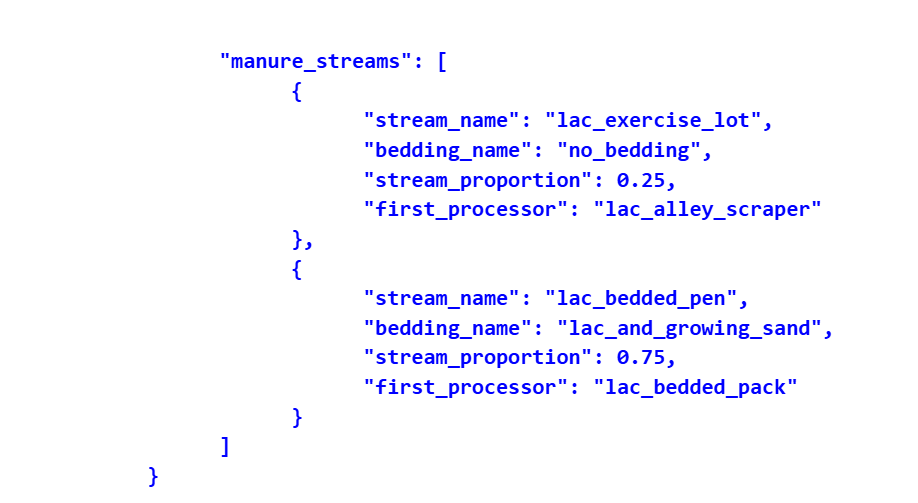
\includegraphics[width=0.9\textwidth]{resources/manurestreams.png} % Replace with your image file
    \caption{If manure from a pen is routed to two different general manure streams, two sets of manure stream inputs must be defined. An example of a single pen’s manure stream inputs is above - in this example, manure from this pen is routed to two locations, one representing an exercise lot, the other representing a bedded pack area.}

    \end{figure}


\textbf{Stream proportion logic}
\vspace{ 0.25cm}

The stream proportion refers to the user-defined proportion (0 to 1) of manure generated by animals in a single pen that enters a specific manure stream. The translation of user-defined stream proportions into the effective stream proportion utilized by the model is described below. This effective proportion is referred to as the split ratio in the model code - it is the value by which total manure excretions are multiplied by to determine the quantity of any single nutrient allocated to a stream of any type (e.g., 20\% (0.20) to parlor stream, 40\% (0.40) to general stream 1, 40\% (0.40) to general stream 2. The values are the split ratios). 

\textbf{Non-lactating pens} If more than one general stream is defined for a single pen, a stream proportion must be provided for each stream, and manure will be allocated to streams according to these proportions. Essentially, the split ratio is equal to the user-defined stream proportion.


\textbf{Lactating pens} 

\textit{Parlor streams}: The user-defined minutes away for milking is used to calculate the stream proportion value for the milking parlor:
\vspace{0.2cm}

\textbf{When:}
    \begin{center}
        \(parlor\_stream\_proportion = \frac{minutes\_away\_for\_milking }{ 1440}\)
    \end{center}
        \vspace{0.5cm}
    
            {\raggedleft \textbf{[AN.PEN.1]}\par}
            \vspace{0.5cm}

    \begin{itemize}
        \item minutes\_away\_for\_milking: user-defined total minutes per day lactating cows spend out of the pen traveling to/from the parlor or being milked.
        \item 1440: minutes per day.

    \end{itemize}

\textit{General streams} Each general stream proportion represents the fraction of manure—excluding that deposited in or during travel to/from the milking parlor—that enters a specific manure stream. For example, if all manure outside the parlor enters one stream, its proportion would be 1.0. If manure outside the parlor was split evenly between two general streams, each stream’s proportion would be 0.50. With this, the effective proportion of total manure entering this stream (the split ratio) must be calculated according to the parlor stream proportion.


First, we determine the proportion of manure entering any and all general streams vs. the parlor stream.
\vspace{0.2cm}

    \begin{center}
        \(total\_general\_stream\_portion = 1 - parlor\_stream\_proportion\)
    \end{center}
        \vspace{0.5cm}
    
            {\raggedleft \textbf{[AN.PEN.2]}\par}
            \vspace{0.5cm}
            
\textbf{When:}
    \begin{itemize}
        \item parlor\_stream\_proportion: proportion of total manure allocated to the parlor stream, calculated in \textbf{[AN.PEN.1]}.
    \end{itemize}

Once we have derived the proportion of manure entering any/all general streams, we multiply this proportion by the user-defined general stream proportion(s), to determine the split ratio for each general stream.
\vspace{0.2cm}

    \begin{center}
        \(general\_stream\_proportion = total\_general\_stream\_proportion * stream\_proportion\)
    \end{center}
        \vspace{0.5cm}
    
            {\raggedleft \textbf{[AN.PEN.3]}\par}
            \vspace{0.5cm}

To continue with our example from above, if cows spent 200 minutes per day in the milking parlor, their split ratios would be as follows: 
\vspace{0.25cm}

\textbf{Parlor:}
\vspace{0.2cm}

\( \frac{200}{1440} = 0.140\)
\vspace{0.1cm}

\(lac\_exercise\_lot: (1 - 0.139) * 0.25 = 0.215\)
\vspace{0.1cm}

\(lac\_bedded\_pen: (1 - 0.139) * 0.75 = 0.645\)
\vspace{0.3cm}

\textbf{Recommended defaults}
\vspace{0.2cm}

Although the time away from a pen is highly variable and specific to each farm’s infrastructure and management, some recommended defaults for situations where actual information is not available are provided below. 
\vspace{0.15cm}

\textit{Minutes away for milking}
\vspace{0.1cm}

Recommended minutes\_away\_for\_milking values for lactating cows are based on cow time budgets from published literature and are not official model defaults. The purpose of these time budgets at the time of writing is strictly related to estimating manure deposition in specific locations and is not related to larger Animal module activities. The use of time budgets for this purpose relies on the assumption that cows excrete urine and feces at a constant rate throughout the day and across various locations.
\vspace{0.1cm}


\clearpage
\begin{sidewaystable}
     \caption{Recommended minutes\_away\_for\_milking by pen type based on published literature. Remember, this does not necessarily reflect the model defaults. }
\centering
\renewcommand{\arraystretch}{1.3}


\begin{tabular}{@{} L{2cm} L{4cm} L{1.5cm} L{8cm} @{}}
\toprule

\multicolumn{1}{c}{\textbf{Pen Type}} & 
\multicolumn{1}{c}{\textbf{minutes\_away\_for\_milking}}  & 
\multicolumn{1}{c}{\textbf{Proportion}}  & 
\multicolumn{1}{c}{\textbf{Special Notes}} \\
\midrule


Freestall\textsuperscript{1} & 200 m (3.33 h) & 0.139 &     \\
Tiestall & 200 m (3.33 h) & 0.139 & Limited data; value is based on the assumption that daily time away from pen for milking will be broadly similar between freestall and tiestall barns.\textsuperscript{2} \\
Open lot & 300 m (5 h) & 0.208 & Assumption that open lot pens tend to be considerably larger than indoor-housed systems (greater travel distance).\textsuperscript{3}
 \\
Compost bedded pack barn & 200 m (3.33 h) & 0.139 & Limited data; value is based on the assumption that daily time away from pen for milking will be broadly similar between freestall and tiestall barns.\textsuperscript{2} \\
\bottomrule
\multicolumn{4}{l}{\footnotesize \textsuperscript{1} \cite{gomez2010time}, \cite{espejo2007herd}} \\
\multicolumn{4}{l}{\footnotesize \textsuperscript{2} \cite{jewell2019prevalence}} \\
\multicolumn{4}{l}{\footnotesize \textsuperscript{3} \cite{meyer2019contract}} \\

\end{tabular}

\end{sidewaystable}





\textit{Open lot and bedded pack systems}
\vspace{0.1cm}

The management of open lot and bedded pack barn pens often results in manure from a single pen being managed in multiple ways. These types of pens often have designated resting areas (i.e. the harrowed lot or bedded pack) where manure is managed in place for an extended period, as well as a separate feeding area, such as a concrete apron along a feed alley. Manure deposited in this area may be scraped back into the resting area, or it may be flushed, vacuumed or scraped to another separate storage area. Two distinct manure management routines within a single pen indicate that two manure streams should likely be used. If this is the case, the user may reference the tables below as a starting point for defining stream proportions representing the resting vs. feeding area. Defining two separate manure streams is recommended where appropriate to ensure that manure is not over-allocated to the parlor manure stream (where it does not contribute to housing emission estimations) and bedding is allocated appropriately. 


The following streams and proportions are based on literature data and are not official model defaults. They are provided for user informational purposes; they may be used as a starting point to adjust proportions specific to a farm, or can be used for theoretical modeling scenarios. 
\vspace{ 0.25cm}


\begin{table}[h!]
\centering
\renewcommand{\arraystretch}{1.3}
\begin{center}
    \caption{Proportions of differnt streams for different animal classes.}
\end{center}
\vspace{-0.5cm}

\begin{tabular}{@{} L{5cm} L{4cm} L{1.2cm} L{1cm} L{0.8cm} L{0.75cm} @{}}
\toprule
\multicolumn{1}{c}{\textbf{Pen Type}} & 
\multicolumn{1}{c}{\textbf{Animal Class}}  & 
\multicolumn{1}{c}{\textbf{Lactating}}  & 
\multicolumn{1}{c}{\textbf{Closeup}}  & 
\multicolumn{1}{c}{\textbf{Growing}}  & 
\multicolumn{1}{c}{\textbf{Calves}} \\


\midrule

\multirow{3}{*}{\textbf{Open lot or bedded pack barn} \textsuperscript{1}} 
& General stream, lot        & 0.796 & 0.76  & 0.76  & 1    \\
& General stream, feed alley & 0.204 & 0.24  & 0.24  & N/A  \\
& minutes\_away\_for\_milking & 300   & N/A   & N/A   & N/A  \\
\cmidrule(lr){1-6}
\multirow{3}{*}{\textbf{Bedded pack barn} \textsuperscript{2}} 
& General stream, bedded pack & 0.792 & 0.819 & 0.819 & 1    \\
& General stream, feed alley  & 0.208 & 0.179 & 0.179 & N/A  \\
& minutes\_away\_for\_milking & 200   & N/A   & N/A   & N/A  \\

\bottomrule
\multicolumn{6}{p{\linewidth}}{\footnotesize\raggedright 
\textsuperscript{1} Based on data from \cite{meyer2019contract} and the assumption that open lot pens tend to be considerably larger than indoor-housed systems (greater travel distance). \par
\textsuperscript{2} Based on data from \cite{endres2007behavior}, which suggests behavior of cows in compost bedded pack barns is broadly similar to those in other housing systems. With this, freestall data from \cite{gomez2010time} was used, which reported 4.3 hours of feeding time, 3.33 hours away for milking, and the remainder spent in the housing area.
} \\


\end{tabular}
\end{table}




\textit{Passing information to the Manure module}
\vspace{0.1cm}

Once split ratios have been determined for each manure stream in each pen, Animal module manure and pen data can be translated into ManureStream objects. The variables contained in ManureStream are below; this dataclass is used both to move information from Animal to Manure module, as well as move information between processors within the Manure module. 


The majority of the variables are calculated in the Animal module and translated directly into a ManureStream object. Subbullets below a variable indicate how variables not directly reported by the Animal module are calculated. 
\vspace{0.2cm}

\textbf{\textit{Bedding}}
\vspace{0.25cm}

Bedding is assigned and applied by manure stream, not by pen. The following calculations described how bedding mass, nutrients, and volume are calculated, and how bedding is added to a manure stream.\\

\textbf{Calculate total bedding mass}
\vspace{ 0.25cm}

calc\_total\_bedding\_mass

\vspace{0.2cm}

    \begin{center}
        \(total\_bedding\_mass (kg) = bedding\_mass\_per\_day (kg/animal) * num\_animals * sand\_removal\_efficiency \)
    \end{center}
        \vspace{0.5cm}
    
            {\raggedleft \textbf{[AN.PEN.7]}\par}
            \vspace{0.5cm}

\textbf{When:}
    \begin{itemize}
        \item bedding\_mass\_per\_day: The user-inputted bedding mass applied per animal per day. Note that this input is per total number of animals housed in the pen.
        \item num\_animals: Animals in the pen from which the manure stream originated.
        \item sand\_removal\_efficiency: User-defined proportion of sand bedding removed via sand settling lane or other sand recovery technology. This value is only utilized if bedding type \= sand.
    \end{itemize}

\textbf{Calculate total bedding volume}
\vspace{ 0.25cm}

calc\_total\_bedding\_volume

\vspace{0.2cm}

    \begin{center}
        \(total\_bedding\_volume (m^3) = \frac{total\_bedding\_mass (kg)}{bedding\_density (kg/m^3)}  \)
    \end{center}
        \vspace{0.5cm}
    
            {\raggedleft \textbf{[AN.PEN.8]}\par}
            \vspace{0.5cm}

\textbf{When:}
    \begin{itemize}
        \item total\_bedding\_mass (kg): the total mass of bedding applied to the manure stream each day, calculated in \textbf{[MN.PEN.7]}.
        \item bedding\_density (kg/m\textsuperscript{3}): user-defined density of the specified bedding.

    \end{itemize}

\textbf{Calculate total bedding dry solids}
\vspace{ 0.25cm}

calc\_total\_bedding\_dry\_solids

\vspace{0.2cm}

    \begin{center}
        \(total\_bedding\_dry\_solids (kg) = total\_bedding\_mass (kg) * bedding\_dry\_matter\_content  \)
    \end{center}
        \vspace{0.5cm}
    
            {\raggedleft \textbf{[AN.PEN.9]}\par}
            \vspace{0.5cm}

\textbf{When:}
    \begin{itemize}
        \item total\_bedding\_mass (kg): the total mass of bedding applied to the manure stream each day, calculated in \textbf{[MN.PEN.7]}.
        \item bedding\_dry\_matter\_content: user-defined dry matter content of the specified bedding.

    \end{itemize}

\textbf{Calculate total bedding water}
\vspace{ 0.25cm}

calc\_total\_bedding\_water

\vspace{0.2cm}

    \begin{center}
        \(total\_bedding\_water (kg) = total\_bedding\_mass (kg) * (1 - bedding\_dry\_matter\_content) \)
    \end{center}
        \vspace{0.5cm}
    
            {\raggedleft \textbf{[AN.PEN.10]}\par}

\textbf{When:}
    \begin{itemize}
        \item total\_bedding\_mass (kg): the total mass of bedding applied to the manure stream each day, calculated in \textbf{[MN.PEN.7]}.
        \item bedding\_dry\_matter\_content: user-defined dry matter content of the specified bedding.

    \end{itemize}
    \vspace{0.5cm}

\textbf{Update ManureStream values to reflect bedding}
\vspace{0.15cm}

\_apply\_bedding (pen.py)
\vspace{0.2cm}

\begin{table}[h!]
\centering
\renewcommand{\arraystretch}{1.3}
\begin{center}
    \caption{Calculated manure and bedding characteristics}
\end{center}
\vspace{-0.2cm}

\begin{tabular}{@{} L{3cm} L{2cm} L{9cm} @{}}
\toprule
\multicolumn{1}{c}{\textbf{Variable}} & 
\multicolumn{1}{c}{\textbf{Units}} & 
\multicolumn{1}{c}{\textbf{Calculation}} \\
\midrule

water  & kg & ManureStream water (kg) + bedding\_water (kg) \\
ash  & kg & if bedding type = sand, ash (kg) = total\_bedding\_mass (kg); otherwise, ash = 0 \\
phosphorus  & kg & ManureStream phosphorus + total\_bedding\_mass (kg) * bedding\_phosphorus\_content) \\
non\_degradable \_volatile\_solids & kg & If bedding type = sand, ManureStream non\_degradable\_volatile\_solids (kg); If bedding type is not sand, ManureStream non\_degradable\_volatile\_solids (kg) + total\_bedding\_dry\_solids (kg) \\
total\_solids  & kg & ManureStream total\_solids (kg) + total\_bedding\_dry\_solids (kg) \\
volume  &  m\textsuperscript{3} & ManureStream volume ( m\textsuperscript{3}) + total\_bedding\_volume ( m\textsuperscript{3}) \\


\bottomrule
\end{tabular}
\end{table}



\section{Manure Handler}
\subsection{Introduction}
    \vspace{0.2cm}
    
    Manure handling refers to the method of managing manure in animal living spaces. For some housing/pen types, such as freestalls and tiestalls, this involves removing the manure from barn alleyways, and is usually accomplished using some form of scraping or flushing with water. Flush systems utilize water to remove the manure from alleyways, whereas scrape systems use little or no water. For other housing types like open lots and compost bedded pack barns, tillage or harrowing are commonly used to instead incorporate the manure, urine, bedding (if applicable) and air into the pack and allow it to dry. 
    \vspace{0.5cm}

    The specific manure handler options in the RuFaS model are:
    \begin{itemize}
        \item \textbf{Flushing} 
        \vspace{0.15cm}

        Flushing involves using water to carry manure and soiled bedding away from housing areas. A series of pipes and channels direct water to wash the manure into a collection pit. Flushing helps maintain a cleaner environment for animals and reduces the buildup of manure on the floor. Flushing/recirculating may also be used to “lubricate” transport/pumping of manure from under-floor collection pits to the next manure management step. Flushing is commonly performed using recycled water from a solid liquid separator, liquid manure storage, or other liquid collection area, rather than using fresh water.

        \item \textbf{Manual Scraping} 
        \vspace{0.15cm}

        Scraping involves physically removing the manure and soiled bedding using equipment like tractor-mounted scrapers or skid steers, or the manual use of shovels/scrapers, etc. This method is typically used in barns with slatted or solid floors. Regular scraping prevents manure accumulation and provides a clean area for animals.

        \item \textbf{Alley Scraper} 
        \vspace{0.15cm}

        A scraper blade, typically pulled along by a chain or cable, moves slowly down a pen or alleyway on a set schedule several times a day, pushing or pulling manure out of the pen/alley. The function and outcome is similar to manual scraping, but alley scrapers are mechanized and typically operate automatically.

        \item \textbf{Parlor Cleaning} 
        \vspace{0.15cm}

        Parlor cleaning is a RuFaS-specific handler that represents cleaning of manure from milking units, parlor stall floors, and other areas in the milking parlor that require the use of fresh, non-recycled water. Parlor cleaning also can include an optional flush system capability, which functions in the same manner as the flush system described above and is used to wash manure from holding area floors.
        
    \end{itemize}




Manure handlers in RuFaS have two primary functions: calculate and add cleaning water if used, and calculate indoor housing emissions of CH\textsubscript{4}, CO\textsubscript{2}, and NH\textsubscript{3} if applicable.
\vspace{0.2cm}

    The following are important assumptions made in the manure handler submodules, as well as context on how manure handlers are used in the larger manure management chain:
    \begin{enumerate}
        \item All manure excreted and all bedding applied each day (if applicable) is assumed to be recovered by the manure handler. 
        \item Manure handlers in RuFaS are intended to be utilized, at this time, with manure deposited in housing areas that is cleaned frequently (e.g., removed daily or every few days), such as indoor barn floors, or concrete feed alleys in open lot or compost bedded pack pens. Handlers should not be used in manure streams where manure resides for a long period of time, such as streams representing an open lot or bedded pack manure pack, that have a designated processor (i.e., Open Lot or Bedded Pack). Users can consider the manure handler functionality to be “built in” to these processors. Defining a handler prior to one of these types of processors will result in double-counting of housing emissions. 
        \item If a manure handler is used, it must be defined first in the manure management chain. This prevents inappropriate calculation of housing emissions “downstream” when manure is no longer in the animal housing area. Handlers are meant to represent manure handling in animal living spaces; other manure handling/transport systems such as pumps, augers, belts, etc. are not explicitly modeled in RuFaS. 
    \end{enumerate}

\newpage
\textbf{Classes}
\vspace{ 0.25cm}

    \begin{table}[h!]
    \begin{center}
        \caption{The classes of handlers that are used in this module.}
    \end{center}
\vspace{ -0.5cm}

    \centering
    \renewcommand{\arraystretch}{1.3}

    \begin{tabular}{@{} L{5cm} L{7cm}  @{}}
    \toprule

    \multicolumn{1}{c}{\textbf{Handlers}} & 
    \multicolumn{1}{c}{\textbf{Description}} \\
    \midrule
    Handler (Processor)  & handler.py contanins basic methods that are applicable to all handlers  \\
    Single StreamHandler (Handler)  & single\_stream\_handler.py contains alley screaper, manual scraping, and flush system-specific methods \\
    ParlorCleaning (Handler)  & parlor\_cleaning.py contains parlor cleaning-specific methods  \\
    \bottomrule
    \end{tabular}
    \end{table}  

\textbf{Required User Inputs }
\vspace{0.25cm}



    \begin{table}[h!]
    \centering
    \renewcommand{\arraystretch}{1.3}
    \begin{center}
        \caption{Required inputs for the Manure Handler (refreshed\_manure\_management.json)}
    \end{center}
    \vspace{-0.2cm}

    \begin{tabular}{@{} L{4.5cm} L{2cm} L{8cm} @{}}
    \toprule
    \multicolumn{1}{c}{\textbf{Variable}} & 
    \multicolumn{1}{c}{\textbf{Units}} & 
    \multicolumn{1}{c}{\textbf{Description}} \\
    \midrule
Name & none &  Unique identifier of the specific handler configuration used. \\ 
Type & none &  The type (alley scraper, manual scraping, flushing, or parlor scraping) of manure handler. \\ 
cleaning\_water\_use\_amount  & L/animal/day &  The rate of water use (L per animal per day, total of fresh and/or recycled water) by a specified manure handler. \\ 
cleaning\_water\_recycle\_fraction & none &  The fraction (0.XX) of cleaning water used by a specified handler that is from recycled (not fresh) water sources. \\ 
use\_parlor\_flush  & true/false &  True/false indication for if a parlor flush (which may be partially or fully recycled water) is used in addition to routine parlor water cleaning with fresh water. \\ 

    \bottomrule
    \end{tabular}
    \end{table}  
    \vspace{ 0.25cm}
    
\textbf{Other inputs}\\
Instance(s) of ManureStream for each manure stream defined by the user that represent the attributes of the manure in the specific manure stream. ManureStream instances include the following variables (all in kg except for volume, \(m^3\) and manure methane potential, \(m^3 / kgVS\)):
    \begin{itemize}
        \item water 
        \item ammoniacal\_nitrogen
        \item nitrogen 
        \item phosphorus
        \item potassium
        \item ash
        \item manure\_degradable\_volatile\_solids
        \item manure\_non\_degradable\_volatile\_solids
        \item bedding\_non\_degradable\_volatile\_solids
        \item total\_solids
        \item mass (equal to sum of water and total solids)
        \item total volatile solids (equal to sum of degradable and non-degradable volatile solids)
        \item volume
        \item methane\_production\_potential

    \end{itemize}

Manure handlers also make use of information contained in the PenManureData subclass. This includes the following information specific to the pen from which the manure was generated:
\begin{itemize}
    \item num\_animals: number of animals in the pen
    \item animal\_combination: type of animals in the pen (calves, growing post-weaning heifers through closeup period), closeup (cows and heifers within user-defined closeup period), or lactating cows)
    \item Manure deposition surface area (m2): surface area soiled with manure. See section below on determining soiled surface area
    \item pen\_type: the type of pen the manure was generated in (freestall, tiestall, open lot, or bedded pack barn)
    \item daily\_urine (kg): mass of urine in the manure
    \item urine\_nitrogen (kg): mass of urine N in the manure
    \item stream\_type: the type of manure stream the manure is in (parlor or general stream)

\end{itemize}
\begin{tcolorbox}[colback=white, colframe=black, boxrule=0.5pt, arc=3pt, width=\textwidth]
Note that stream\_type is not a user input, it is automatically assigned. Parlor streams are created automatically and all other streams are assigned “general”.
\end{tcolorbox}


\textbf{Expected Outputs}
\vspace{ 0.25cm}
\begin{itemize}
    \item All handler types:
    \begin{itemize}
        \item ManureStream variables
        \item total\_cleaning\_water\_volume ( m\textsuperscript{3}): total volume of fresh (non-recycled) cleaning water used for, and ultimately added to, a single manure stream on a single simulation day by the manure handler
        \item barn\_temperature (\(\circ C\)): ambient temperature in barn
    \end{itemize}
    \item Alley scraper, manual scraping, flush system:
    \begin{itemize}
        \item housing\_methane (kg): daily CH\textsubscript{4} (kg) emitted from manure on barn floors
        \item housing\_ammonia\_N\_emissions: (kg): daily NH\textsubscript{3}-N (kg) emitted from manure on barn floors
        \item housing\_carbon\_dioxide (kg): daily CO\textsubscript{2} (kg) emitted from manure on barn floors
    \end{itemize}

\end{itemize}


\subsection{Methodology}


\textbf{Calculate barn temperature}
\vspace{ 0.25cm}

\_determine\_barn\_temperature

Air temperature inside barns is, in general, slightly cooler than the outdoors during the day, and slightly-to-considerably warmer than the outdoor temperature overnight, depending on the season. With this, basic bounds were implemented in the determination of barn temperature. These bounds were suggested by manure SMEs and are supported by barn temperature ranges reported in \cite{Bucklin2009} (Florida, upper limit). The lower bound (5$^\circ$C) suggested by SMEs was based on general industry standards/conditions.

\vspace{ 0.25cm}
If ambient (outdoor) air temperature \(<\) 5$^\circ$C, barn temperature = 5$^\circ$C\\
If ambient (outdoor) air temperature \(>\) 5$^\circ$ \& \(<\) 30$^\circ$C, barn temperature = air temperature\\
If ambient (outdoor) air temperature \(>\) 30$^\circ$C, barn temperature = 30$^\circ$C\\


\textbf{Calculate cleaning/flushing fresh water addition}
\vspace{ 0.25cm}

determine\_handler\_cleaning\_water\_volume

The following method calculates the volume of fresh (non-recycled) cleaning water used for, and ultimately added to, a single manure stream on a single simulation day by the manure handler. This method is used in all handler types; however, for parlor cleaning handlers, this method is only utilized if “use\_parlor\_flush” is entered as true. If no water is used with the handler (user inputted cleaning water use rate = 0), the function will return 0.
\vspace{0.2cm}

    \begin{center}
        \(cleaning\_water \ (L) = num\_animals * (cleaning\_water\_use\_rate * (1 - cleaning\_water\_recycle\_fraction)) \)
    \end{center}
        \vspace{0.5cm}
    
            {\raggedleft \textbf{[MN.HDL.1]}\par}
            \vspace{0.5cm}

\textbf{When:}
    \begin{itemize}
        \item num\_animals: the number of animals in the pen assigned to the handler
        \item cleaning\_water\_use\_rate (L/animal/d): the user-provided cleaning water use rate for the handler
        \item cleaning\_water\_recycle\_fraction: the proportion of cleaning water that is from recycled, non-fresh sources

    \end{itemize}  
    \vspace{0.2cm}
    
Total fresh water added to manure (L) each day is calculated as follows: 
\vspace{0.2cm}

    \begin{center}
        \(total\_cleaning\_water (m^3) = (cleaning\_water (L) + fresh\_water\_volume\_used\_for\_milking (L)) * LITERS\_TO\_CUBIC\_METERS\)
    \end{center}
        \vspace{0.5cm}
    
            {\raggedleft \textbf{[MN.HDL.2]}\par}
            \vspace{0.25cm}
\textbf{When:}
    \begin{itemize}
        \item LITERS\_TO\_CUBIC\_METERS: a constant set to 0.997 kg/m\textsuperscript{3}

    \end{itemize}  

 
\textbf{Calculate milking parlor fresh water addition}
\vspace{ 0.25cm}

The following method calculates the volume of fresh water used for, and ultimately added to, a single manure stream on a single simulation day by the manure handler for parlor cleaning/sanitation purposes. This calculation occurs only in the parlor\_cleaning handler and water added is considered to be 100\% fresh, non-recycled water, as fresh water is required for cleaning of milking units, floors, etc. The following function is implicit (occurs automatically with any manure stream assigned to the parlor cleaning handler type) and is based at this time on a default value fresh water use rate. 
\vspace{0.2cm}

    \begin{center}
        \(fresh\_water\_volume\_used\_for\_milking\ (L) = num\_animals\ *\ MILKING\_FRESH\_WATER\_USE\_RATE 
 \)
    \end{center}
        \vspace{0.5cm}
    
            {\raggedleft \textbf{[MN.HDL.3]}\par}
            \vspace{0.5cm}

\textbf{When:}
    \begin{itemize}
        \item num\_animals: the number of animals in the pen assigned to the handler
        \item MILKING\_FRESH\_WATER\_USE\_RATE (30.0 L/animal/d): the default fresh water use rate for cleaning equipment/floors in the milking parlor
    \end{itemize}  

\textbf{Calculate housing emissions}
\vspace{ 0.25cm}

The calculation of housing emissions according to the methods described below is applicable only to areas where manure resides for short periods of time, i.e., tiestall and freestall housing systems, or, in open lot or bedded pack pens, manure deposited in a feed alley, exercise lot, etc. Housing emissions from bedded packs and open lot manure packs, where manure accumulates over weeks or months, are determined according to alternative methods due to the longer-term residence of manure in these pen types; see respective bedded pack barn and open lot documentation files for further info. 

\vspace{ 0.25cm}
The methodology used to calculated housing emissions is adapted from the IFSM \parencite{Rotz2023}. Of note is that the equations described here were determined based on emissions in tiestall and freestall housing systems. In RuFaS, these equations may also be applied to determine emissions from manure deposited in other concrete areas and retained for a short time, such as open lot or bedded pack feed alleys. These systems were not represented in the original datasets used to generate these equations, and results should be interpreted with caution; however, the portion of manure deposited in feed alleys or other areas is relatively small, and emissions from this area are expected to be a small contributor to total GHG and nutrient losses.

\vspace{ 0.25cm}
Additionally, the following calculations are only utilized by the manual scraping, flush system, and alley scraper handler types. For the parlor cleaning handler type, manure in a parlor is assumed to be cleaned from floors/surfaces frequently and thus housing emissions should not be estimated. 

\vspace{ 0.25cm}
\textbf{Calculate housing CH\textsubscript{4} emissions}
\vspace{ 0.25cm}

Manure deposited on barn floors or other housing areas is a small source of CH\textsubscript{4} emissions. The following method, from \cite{Chianese2009a}, is an empirically-derived equation consisting of a simple relationship between manure CH\textsubscript{4} emission rate, ambient temperature in the barn, and surface area covered by manure. 
\begin{tcolorbox}[colback=white, colframe=black, boxrule=0.5pt, arc=3pt, width=\textwidth]
The soiled surface area (m2) value is calculated in the Animal module, using pen-level information (number of stalls, number of cows, etc.) and the soiled surface area value is passed to the manure module directly. As no housing emissions are considered to be emitted in the milking parlor, the total soiled surface area for each pen is apportioned to the pen's general manure streams(s) based on the user-provided stream proportion value(s).
\end{tcolorbox}


    \begin{table}[h!]
    \centering
    \renewcommand{\arraystretch}{1.3}
    \begin{center}
        \caption{The surface area per stall that is covered with manure is a function of the pen type and type of animal housed.}
    \end{center}
    \vspace{-0.5cm}
    
    \begin{tabular}{@{} C{2cm} C{3cm} C{3cm}  @{}}
    \toprule
    \multicolumn{1}{c}{\textbf{System Type}} & 
    \multicolumn{1}{c}{\textbf{Lactating Cows}} & 
    \multicolumn{1}{c}{\textbf{Closeup, Growing, or Calves}} \\
    \midrule
    Tiestall  & 1.2  m\textsuperscript{2} & 1.0  m\textsuperscript{2}  \\
    Freestall  & 3.5  m\textsuperscript{2} & 2.5  m\textsuperscript{2}  \\
    Bedded Pack  & 5.0  m\textsuperscript{2} & 5.0  m\textsuperscript{2}  \\
    Open Lot  & 3.0  m\textsuperscript{2} & 3.0  m\textsuperscript{2}  \\
    \bottomrule
    \end{tabular}
    \end{table} 
\vspace{0.2cm}

The total surface area soiled with manure, based on the total number of animals, is as follows:
\vspace{0.2cm}

    \begin{center}
        \(soiled\_surface\_area\ (m^2) = num\_stalls * surface\_area\ (m^2/animal)
 \)
    \end{center}
        \vspace{0.5cm}
    
            {\raggedleft \textbf{[MN.HDL.4]}\par}
            \vspace{0.5cm}

\textbf{When:}
    \begin{itemize}
        \item num\_stalls: the number of stalls in the pen assigned to the handler
         \item surface\_area (m\textsuperscript{2}/animal): surface area per stall, provided in Table 8.
    \end{itemize}  

We use this surface area value to determine CH\textsubscript{4} emissions (kg) each day
\vspace{0.2cm}

    \begin{center}
        \(housing\ CH_{4}\ (kg) = max^1(0.0, 0.13 * barn\_temperature (C)) * \frac{soiled\_surface\_area\ (m^2)}{1000}
 \)
    \end{center}
        \vspace{0.5cm}
    
            {\raggedleft \textbf{[MN.MET.1]}\par}
            \vspace{0.5cm}

\textbf{When:}
    \begin{itemize}
        \item barn\_temperature (\(^\circ C\)): ambient air temperature in the barn. Note that the max notation ensures that the temperature scaling parameter cannot be less than 0.13.
        \item soiled\_surface\_area (m\textsuperscript{2}): the total surface area soiled with manure
    \end{itemize}  


\textbf{Calculate housing CO\textsubscript{2} emissions}
Housing CO\textsubscript{2} emissions are estimated similarly to CH\textsubscript{4} emissions, using an empirical equation based on soiled surface area and barn air temperature.
\vspace{0.2cm}

    \begin{center}
        \(housing\ CO_{2}\ (kg) = max^1(0.0, 0.0065 + barn\_temperature (C)) * soiled\_surface\_area\ (m^2)
 \)
    \end{center}
        \vspace{0.5cm}
    
            {\raggedleft \textbf{[MN.HDL.5]}\par}
            \vspace{0.5cm}

\textbf{When:}
    \begin{itemize}
        \item barn\_temperature (\(^\circ C\)): ambient air temperature in the barn. Note that the max notation ensures that the temperature scaling parameter cannot be less than 0.13.
        \item soiled\_surface\_area (m\textsuperscript{2}): the total surface area soiled with manure
    \end{itemize}  
            
\textbf{Calculate volatile solids losses}
The total quantity of VS loss through microbial degradation is estimated based on CH\textsubscript{4} emissions.
 \vspace{0.2cm}

    \begin{center}
        \(total\_VS\_loss\ (kg) = housing\ CH_4\ (kg)  * VS\_TO\_METHANE\_LOSS\_RATIO\)
    \end{center}
        \vspace{0.5cm} 
    
            {\raggedleft \textbf{[MN.HDL.6]}\par}
            \vspace{0.5cm}

\textbf{When:}
    \begin{itemize}
        \item housing CH\textsubscript{4} (kg): daily emissions of CH\textsubscript{4} from manure on barn floors, calculated in \textbf{[MN.MET.1]}.
        \item VS\_TO\_METHANE\_LOSS\_RATIO (kg): a constant set to 6.665 representing the kg of total VS degraded per kg of CH\textsubscript{4} emitted from manure. See the Slurry Storage section for more information on derivation of this constant.
    \end{itemize}  


The fraction of volatile solids lost from the manure degradable (VSd) and non-degradable VS (VSnd) fractions is assumed to be equal to the proportion of these fractions in manure entering the processor. No VS losses are attributed to bedding VSnd in manure handlers.
 \vspace{0.2cm}

    \begin{center}
\(degradable\_VS\_frac = (\frac{degradable\_VS}{total\_VS}) \)
    \end{center}
        \vspace{0.5cm} 
    
            {\raggedleft \textbf{[MN.ADG.7]}\par}
            \vspace{0.5cm}

\textbf{Calculate housing NH\textsubscript{3} emissions}
Ammonia N loss from manure is predicted using methods based on \cite{Rotz2006}. Here, estimated NH\textsubscript{3}-N volatilized from the surface of manure is based on a function where the NH\textsubscript{3}-N is transported to the free atmosphere through a pathway with a finite resistance. Daily NH\textsubscript{3}-N loss depends primarily on pen type (which determines soiled surface area), manure TAN content, and barn air temperature. The same base equation for NH\textsubscript{3}-N volatilization is utilized for estimation of both housing and storage NH\textsubscript{3}-N emissions. 
\vspace{0.2cm}

In the original work of \cite{Rotz2006}, housing NH\textsubscript{3}-N emissions are based only on urine (not manure) TAN concentration, rather than total manure (urine + feces) TAN. Within RuFaS, urine nutrients are not tracked separately from feces/manure. Therefore, the model assumes, for simplicity, that all TAN originates from urine and thus animal-excreted urine TAN = manure TAN. However, to maintain consistency with documentation, what would ordinarily in RuFaS be referred to as manure TAN within RuFaS is referred to here as urine TAN, though urine mass here (kg/d) is reflective of actual estimated urine mass, not manure (urine + feces) mass.
\vspace{0.5cm}

    \begin{itemize}

        \item \hypertarget{HENRY}{First}, we need to derive the value of the equilibrium coefficient Q for the NH\textsubscript{3} gas in the air for a given concentration of TAN in stored slurry using Henry’s law of distribution. 
    \end{itemize}
    \vspace{0.15cm}

\begin{tcolorbox}[colback=white, colframe=black, boxrule=0.5pt, arc=3pt, width=\textwidth]
The concentration of NH\textsubscript{3} in the free atmosphere is assumed to be zero. Since Q is a function of the Henry’s law coefficient K\textsubscript{h} and a dissociation of ammonium coefficient K\textsubscript{a}, we will calculate those first.
\end{tcolorbox}
        \vspace{0.2cm}
        
         Henry’s law coefficient (K\textsubscript{h})
         \vspace{0.2cm}

    \begin{center}
\(K_h = 10 ^\frac{1478} {barn\ temperature - 1.69} \)
    \end{center}
        \vspace{0.5cm} 
    
            {\raggedleft \textbf{[MN.AMM.1]}\par}
            \vspace{0.5cm}
            
\textbf{When:}
    \begin{itemize}
        \item Barn temperature (K): ambient air temperature in the barn 
    \end{itemize}

         Dissociation coefficient of ammonium (K\textsubscript{a})
         \vspace{0.2cm}

    \begin{center}
\(K_a  = 1 + 10 ^{(0.09018 + (\frac{2729.9} {barn\ temperature} - pH )}\)
    \end{center}
        \vspace{0.5cm} 
    
            {\raggedleft \textbf{[MN.AMM.2]}\par}
            \vspace{0.5cm}

\textbf{When:}
    \begin{itemize}
        \item Barn temperature (K): ambient air temperature in the barn
        \item pH: the pH of the manure solution, set to 7.5 by default

    \end{itemize}

        
        Equilibrium coefficient (Q)
         \vspace{0.2cm}

    \begin{center}
\(Q = K_h * K_a \)
    \end{center}
        \vspace{0.5cm} 
    
            {\raggedleft \textbf{[MN.AMM.3]}\par}
            \vspace{0.5cm}

\textbf{When:}
    \begin{itemize}
        \item K\textsubscript{h}: Henry’s law coefficient, calculated in \textbf{[MN.AMM.1]}.
        \item K\textsubscript{a}: Dissociation coefficient of ammonium, calculated in \textbf{[MN.AMM.2]}.
    \end{itemize}
    \vspace{0.5cm}
    
    \begin{itemize}
        \item Second, we determine the effective total resistance value of NH\textsubscript{3} transport from manure solution to the surface and from the manure surface to the atmosphere. 
         \vspace{0.2cm}

    \begin{center}
\(ammonia\_resistance = HOUSING\_SPECIFIC\_CONSTANT * (1 - 0.027 * (20.0 - barn\ temperature)) \)
    \end{center}
        \vspace{0.5cm} 
    
            {\raggedleft \textbf{[MN.AMM.4]}\par}
            \vspace{0.5cm}

\textbf{When:}
    \begin{itemize}
        \item HOUSING\_SPECIFIC\_CONSTANT: a housing-specific constant value, set to 260 s/m.
        \item Barn temperature (\(^\circ C\)): ambient air temperature in the barn.

    \end{itemize}

        \item Next, the rate of NH\textsubscript{3}-N loss in kg N/m\textsuperscript{2} from manure on the barn floor is calculated 
         \vspace{0.2cm}

    \begin{center}
\(NH_3N\ emission\ rate\ (kg\ N/m^2)= \frac{(TAN * c * y)}{(r * M * Q)} \)
    \end{center}
        \vspace{0.5cm} 
    
            {\raggedleft \textbf{[MN.AMM.5]}\par}
            \vspace{0.5cm}

\textbf{When:}
    \begin{itemize}
        \item TAN (kg N/m\textsuperscript{2}): Mass of ammoniacal N in barn floor manure
        \item c: time conversion constant (86400 s per d)
        \item y: manure density, set to 990 kg/m\textsuperscript{3} 
        \item r: the resistance of NH\textsubscript{3} transfer from solution to manure surface, and from manure surface to atmosphere, determined in \textbf{[MN.AMM.4]}
        \item M: urine mass (received from animal module)
        \item Q: equilibrium coefficient, calculated in \textbf{[MN.AMM.3]}

    \end{itemize}

        \item Lastly, we calculate total NH\textsubscript{3}-N emissions (kg), based on the emission rate we just calculated and the soiled surface area. 
         \vspace{0.2cm}

    \begin{center}
\(NH_3N\ emissions\ (kg) = NH_3N\_rate * soiled\_surface\_area \)
    \end{center}
        \vspace{0.5cm} 
    
            {\raggedleft \textbf{[MN.AMM.7]}\par}
            \vspace{0.5cm}

\textbf{When:}
    \begin{itemize}
        \item NH\textsubscript{3}N\_rate (kg N/m\textsuperscript{2}): Rate of NH\textsubscript{3}-N loss (kg/m\textsuperscript{2}) from manure, calculated in \textbf{[MN.AMM.5]}
        \item soiled\_surface\_area (m\textsuperscript{2}): the total surface area soiled with manure

    \end{itemize}
        
    \end{itemize} 

\subsection{Manure composition update}
Below is a summary of updates to ManureStream variables. 
\vspace{0.2cm}

\begin{tcolorbox}[colback=white, colframe=black, boxrule=0.5pt, arc=3pt, width=\textwidth]
The formulas below may be a summarization of multiple steps detailed above, and are intended to provide an overview of what mass losses/gains are reflected in the value of each variable.
\end{tcolorbox}
\vspace{0.2cm}

Equations in the table below are in the format of “Output/exiting value” = “Entering processor value” +/- XYZ. “Entering” refers to the manure entering the processor (i.e., being loaded into the digester) and output variables reflect the manure leaving the processor (i.e., digestate leaving the digester). The Calculation column describes how the variable is updated in the processor.

\renewcommand{\arraystretch}{1.3}
\begin{table}[h!]
\centering
\caption{Calculated manure storage variables and their units}
\begin{tabular}{@{} L{5cm} L{1cm} L{9cm} @{}}
\toprule

\multicolumn{1}{c}{\textbf{Variable}} & 
\multicolumn{1}{c}{\textbf{Units}} & 
\multicolumn{1}{c}{\textbf{Calculation}} \\
\midrule

water  & kg & \( \text{Entering water (kg)} + (\text{total\_cleaning\_water (m}^3) \times \text{WATER\_DENSITY\_KG\_PER\_M3}) \) \\
total\_ammoniacal\_nitrogen  & kg & \( \min(0, \text{entering ammoniacal\_nitrogen (kg)} - \text{NH\textsubscript{3}-N emissions (kg)}) \) \\
nitrogen  & kg & \( \min(0, \text{entering nitrogen (kg)} - \text{NH\textsubscript{3}-N emissions (kg)}) \) \\
phosphorus  & kg & \( \text{Entering phosphorus (kg)} \) \\
potassium  & kg & \( \text{Entering potassium (kg)} \) \\
ash  & kg & \( \text{Entering ash (kg)} \) \\
non\_degradable\_volatile\_solids &  & \( \text{Entering non\_degradable\_volatile\_solids} - (\text{total\_VS\_loss} \times (1 - \text{degradable\_VS\_frac})) \) \\
degradable\_volatile\_solids &  & \( \text{Entering degradable\_volatile\_solids} - (\text{total\_VS\_loss} \times \text{degradable\_VS\_frac}) \) \\
total\_solids  & kg & \( \text{Entering total\_solids} - \text{total\_VS\_loss} \) \\
volume  & m\textsuperscript{3} & \( \frac{\text{Entering volume} - \text{total\_VS\_loss}}{\text{ManureConstants.SLURRY\_MANURE\_DENSITY}}^{1,2} \) \\


\bottomrule
\multicolumn{3}{l}{\textsuperscript{1} WATER\_DENSITY\_KG\_PER\_M3: a constant with a value of 0.997 kg/m\textsuperscript{3}.}\\
\multicolumn{3}{l}{\textsuperscript{2} Note that for parlor cleaning handlers, the value of all housing emissions variables will be reported as 0.} \\
\end{tabular}

\end{table}


 


\section{Solid Liquid Separators} 
\subsection{Introduction} A solid-liquid separator (SLS) is a specialized piece of equipment or system designed to separate larger, solid particles from the liquid component of manure. This type of system may be implemented for a variety of reasons, such as to improve ease of handling of manure liquid, improve the nutrient concentration in manure liquid, reduce storage volume required for manure lagoons or other storage systems, prevent solid accumulation in a covered manure storage, or reclaim manure solids for use as bedding or compost. 
    
The solid fraction of manure slurry is composed of fibers originating primarily from manure, but also from feed, bedding, and other environmental sources. Once mechanically separated, the moisture content of the solid fraction ranges from 70\% to 90\%, depending on the specific separator system used. To further reduce moisture content of the separated solids, an additional dewatering or drying step may be incorporated. Manure solids may be directly used or sold for animal bedding (after stabilization), composted, or land applied. 
    
After the manure solids are mechanically separated, the remaining liquid fraction is composed of small particles, water, and most of the nutrients present in the manure. Because the bulk of relevant nutrients (e.g., P, N, K) are mainly associated with the small particles which remain with the liquid fraction after separation occurs, separating the larger, less nutrient-dense particles out from the slurry liquid enriches the concentration of these nutrients in the liquid fraction. Solid-liquid separation also makes the manure slurry easier to pump, transport, and apply to fields, as large particles that may clog lines and sprayers are removed.
\vspace{0.5cm}

\textbf{Implementation in RuFaS}
\vspace{ 0.25cm}
    
In RuFaS, solid liquid separators currently represent mechanical, short retention time pieces of equipment. GHG emissions and other nutrient transformations from long-retention separators such as weeping walls or settling basins are not yet represented in the model. Because of this, the impact of these longer retention separators can only be approximated via modification of the separation efficiencies of the short retention time methods.
\vspace{0.15cm}

Currently, SLS inputs are simply nutrient-specific separation efficiencies that reflect the proportion of a specific nutrient that is separated into the solids fraction. With this, essentially any type of mechanical manure separation system can be modeled, as long as effective separation efficiencies are known. Manure is assumed to be loaded, processed, and passed to the next processor within a single day. Default separation efficiencies exist for two common types of SLS - a screw press and a rotary screen. The separated manure solids and remaining liquid fraction are quantified and can be managed in separate, downstream manure management systems in RuFaS. However, separated solids cannot be directly recycled (i.e., utilized with the specific nutrient composition of those separated solids) “upstream” as bedding.  
\vspace{0.5cm}

\textbf{Classes}
    \begin{table}[h!]
    \centering
    \renewcommand{\arraystretch}{1.3}

    \begin{center}
        \caption{List of Python classes for solid liquid separators.}
    \end{center}
    \vspace{0.2cm}
    
    \begin{tabular}{@{} C{3cm} C{4.5cm}  @{}}
    \toprule
    \textbf{Handlers} & \textbf{Description}   \\
    \midrule
    Separator (Processor)  & separator.py  \\

    \bottomrule
    \end{tabular}
    \end{table}

\textbf{Required User Inputs }
    \vspace{0.2cm}


\begin{longtable}{@{} L{4.5cm} L{2cm} L{8cm} @{}}
\caption{The required inputs of this section.} \\

\toprule
\textbf{Variable} & 
\textbf{Definition (units)} & 
\textbf{Description} \\
\midrule
\endfirsthead

\toprule
\textbf{Variable} & 
\textbf{Definition (units)} & 
\textbf{Description} \\
\midrule
\endhead

\bottomrule
\endfoot
 Name & none &  Unique identifier of the specific separator configuration used. \\ 
type & rotary screen or screw press &  The type of solid liquid separator ; selection of this input indicates which default separations efficiencies should be used, however, any and all separation efficiencies may also be overwritten by user input. \\ 
separated\_solids\_dry\_matter & none &  percent dry matter by mass of the manure solids post solid-liquid separation. \\ 
total\_solids\_efficiency & none &  the proportion of manure total solids (TS) that are separated into the manure solids fraction by the separator. \\ 
 volatile\_solids\_efficiency & none &  the proportion of manure volatile solids (VS) that are separated into the manure solids fraction by the separator. \\ 
 nitrogen\_efficiency & none &  the proportion of manure total nitrogen that is separated into the manure solids fraction by the separator. \\ 
 ammoniacal\_nitrogen\_efficiency & none &  the proportion of manure ammoniacal nitrogen that is separated into the manure solids fraction by the separator. \\ 
 phosphorus\_efficiency & none &  the proportion of manure phosphorus that is separated into the manure solids fraction by the separator. \\ 
 potassium\_efficiency & none &  the proportion of manure potassium that is separated into the manure solids fraction by the separator. \\ 
 ash\_efficiency & none &  the proportion of manure ash that is separated into the manure solids fraction by the separator. \\ 

    \end{longtable}  
    \vspace{0.5cm}
    
\textbf{Other inputs}
    \vspace{ 0.25cm}

Instance(s) of ManureStream for each manure stream defined by the user that represent the attributes of the manure in the specific manure stream. ManureStream instances include the following variables (all in kg except for volume, \(m^3\) and manure methane potential, \(m^3 / kgVS\)):
    \begin{itemize}
        \item water 
        \item ammoniacal\_nitrogen
        \item nitrogen 
        \item phosphorus
        \item potassium
        \item ash
        \item manure\_degradable\_volatile\_solids
        \item manure\_non\_degradable\_volatile\_solids
        \item bedding\_non\_degradable\_volatile\_solids
        \item total\_solids
        \item mass (equal to sum of water and total solids)
        \item total volatile solids (equal to sum of degradable and non-degradable volatile solids)
        \item volume
        \item methane\_production\_potential
    \end{itemize}
    \vspace{0.5cm}  

    \textbf{Expected Outputs}
    \vspace{ 0.25cm}

    \begin{itemize}
        \item Two sets of ManureStream variables, representing the separated solids (“SeparatedSolids”) and liquid fraction (“SeparatedLiquid”), respectively

    \end{itemize}
    \vspace{0.2cm}

\subsection{Methodology}


\textbf{Separate nutrients}
\vspace{ 0.25cm}

The equations below describe the general process for separating nutrients between liquid and solid fractions. The general equation for nutrient removal is as follows:
         \vspace{0.2cm}

    \begin{center}
\(Separated\ solids\ nutrient\ content = received\ manure\ nutrient * separation\ efficiency \)
    \end{center}
        \vspace{0.5cm} 
    
            {\raggedleft \textbf{[MN.SEP.1]}\par}
            \vspace{0.5cm}

    \begin{center}
\(Separated\ liquid\ nutrient\ content = received\ manure\ nutrient * (1 - separation efficiency)\)
    \end{center}
        \vspace{0.5cm} 
    
            {\raggedleft \textbf{[MN.SEP.2]}\par}
            \vspace{0.5cm}

\textbf{When:}
    \begin{itemize}
        \item Received manure nutrient (kg): quantity of the specific nutrient in manure being loaded into the separator on a single day. 
    \end{itemize}
    \vspace{0.2cm}
    
\vspace{0.2cm}

Nutrients that are separated according to this pattern are presented in the table below. The default separation efficiencies, as well as minimum and maximum allowable separation efficiencies, for the rotary screen and screw press separators are also provided \parencite{Hegg1981, Mukhtar1999, Varma2021}. Note that separate removal efficiencies for manure degradable and non-degradable VS or bedding non-degradable VS are not specifiable at this time; all VS fractions are assumed to be removed at the rate of total VS removal. 
\newpage

    \begin{table}[h!]
    \centering
    \renewcommand{\arraystretch}{1.3}
    \begin{center}
        \caption{The default, minimums, and maximums for various separation efficiencies.}
    \end{center}
    \vspace{-0.2cm}
    
    \begin{tabular}{@{}  L{3cm} L{3cm} L{2cm} L{2cm} L{2cm}   @{}}
    \toprule

        \multicolumn{1}{c}{\textbf{Type}} & 
        \multicolumn{1}{c}{\textbf{Variable}} & 
        \multicolumn{1}{c}{\textbf{Default}} & 
        \multicolumn{1}{c}{\textbf{Min}} & 
        \multicolumn{1}{c}{\textbf{Max}} \\


    
    \midrule
\multirow{7}{*}{Rotary Screen} 
  & Total solids       & 0.35 & 0.25 & 0.4 \\
  & Nitrogen           & 0.3  & 0.25 & 0.35 \\
  & Ammoniacal N       & 0.15 & 0.1  & 0.2 \\
  & Phosphorus         & 0.4  & 0.3  & 0.45 \\
  & Potassium          & 0.15 & 0.05 & 0.2 \\
  & Ash                & 0.2  & 0.05 & 0.3 \\
  & Volatile solids    & 0.35 & 0.3  & 0.45 \\

\multirow{7}{*}{Screw Press}
  & Total solids       & 0.25 & 0.15 & 0.35 \\
  & Nitrogen           & 0.3  & 0.2  & 0.35 \\
  & Ammoniacal N       & 0.15 & 0.05 & 0.2 \\
  & Phosphorus         & 0.2  & 0.1  & 0.35 \\
  & Potassium          & 0.23 & 0.15 & 0.35 \\
  & Ash                & 0.2  & 0.05 & 0.3 \\
  & Volatile solids    & 0.25 & 0.2  & 0.4 \\

\bottomrule
\multicolumn{5}{l}{\textsuperscript{1} \parencite{Jorgensen2009, Fournel2019}} \\
\end{tabular}

\end{table}
\vspace{0.2cm}

    
\textbf{Calculate total mass and water}
\vspace{ 0.25cm} 

\textit{Separated solids fraction}
\vspace{ 0.25cm} 
Total mass of the separated solids fraction is determined by dividing the mass of separated solids by the user-inputted separated solids dry matter content. 
         \vspace{0.2cm}

    \begin{center}
        \(Separated\ solids\ mass\ (kg)  = \frac{Separated\ solids\ TS\ (kg)} {Separated\ solids\ \%DM}\)
    \end{center}
        \vspace{0.5cm} 
    
            {\raggedleft \textbf{[MN.SEP.3]}\par}
            \vspace{0.5cm}

\textbf{When:}
    \begin{itemize}
        \item Separated solids TS (kg): the mass of solids in the separated manure solids fraction
        \item Separated solids \%DM: user-inputted separated solids dry matter content

    \end{itemize}
    \vspace{0.3cm}
    
The mass of water in the separated solids fraction can then be determined as follows, given the assumption that total mass is equal to the sum of solids plus water:
         \vspace{0.2cm}

    \begin{center}
        \(Separated\ solids\ water\ (kg)  = Separated\ solids\ mass\ (kg) - Separated\ solids\ TS\ (kg)\)
    \end{center}
        \vspace{0.5cm} 

\textit{Separated liquid fraction}
\vspace{ 0.25cm} 

The total mass of the separated liquid fraction, as well as the mass of water, are simply equal to the mass and water in manure loaded into the separator, minus the quantity of each respective value partitioned into the separated solids fraction. 
         \vspace{0.2cm}

\begin{center}
        \(Separated\ solids\ mass\ (kg)  = Received\ mass\ (kg) - Separated\ solids\ mass\ (kg)
        Separated\ solids\ water\ (kg)  = Received\ water\ (kg) - Separated\ solids\ water\ (kg)\)
    \end{center}


\vspace{0.2cm}
            
\textbf{Calculate volume}
\vspace{0.2cm}

Volume of each separated fraction is determined by dividing the mass of each fraction by its respective density:
         \vspace{0.2cm}

    \begin{center}
\(Separated\ solids\ volume\ m^3  = \frac{Separated\ solids\ mass}{SOLID\_MANURE\_DENSITY} \)

    \end{center}
        \vspace{0.5cm} 
    
            {\raggedleft \textbf{[MN.SEP.4]}\par}
            \vspace{0.5cm}

    \begin{center}

\(Separated\ liquid\ volume\ m^3 = \frac{Separated\ liquid\ mass}{LIQUID\_MANURE\_DENSITY} \)
    \end{center}
        \vspace{0.5cm} 
    
            {\raggedleft \textbf{[MN.SEP.5]}\par}
            \vspace{0.5cm}

\textbf{When:}
    \begin{itemize}
        \item SOLID\_MANURE\_DENSITY (kg/ m\textsuperscript{3}): The default density of solid manure, set to 700 kg/ m\textsuperscript{3}\\
        \item LIQUID\_MANURE\_DENSITY(kg/ m\textsuperscript{3}): The default density of liquid manure, set to 900 kg/ m\textsuperscript{3}\\
    \end{itemize}
    \vspace{0.2cm}

\subsection{Manure composition update}
\vspace{0.2cm}

Below is a summary of updates to ManureStream variables. Note that the formulas below may be a summarization of multiple steps detailed above, and are intended to provide an overview of what mass losses/gains are reflected in the value of each variable.

Equations in the table below are in the format of “Output/exiting value” = “Entering processor value” +/- XYZ. “Entering” refers to the manure entering the processor (i.e., being loaded into the digester) and output variables reflect the manure leaving the processor (i.e., digestate leaving the digester). The Calculation column describes how the variable is updated in the processor.


\renewcommand{\arraystretch}{1.3}
\begin{longtable}{@{} L{3.5cm} L{1cm} L{6cm} L{6cm} @{}}
\caption{Solids and liquid fraction calculations for separated manure components} \\
\toprule
\multicolumn{1}{c}{\textbf{Variable}} & 
\multicolumn{1}{c}{\textbf{Units}} & 
\multicolumn{1}{c}{\textbf{Calculation (Solids Fraction)}} & 
\multicolumn{1}{c}{\textbf{Calculation (Liquid Fraction)}} \\
\midrule
\endfirsthead

\toprule
\multicolumn{1}{c}{\textbf{Variable}} & 
\multicolumn{1}{c}{\textbf{Units}} & 
\multicolumn{1}{c}{\textbf{Calculation (Solids Fraction)}} & 
\multicolumn{1}{c}{\textbf{Calculation (Liquid Fraction)}} \\
\midrule
\endhead

\bottomrule
\multicolumn{4}{r}{\textit{Continued on next page}} \\
\endfoot

\bottomrule
\endlastfoot

water  & kg & 
\( \text{Separated solids mass (kg)} - \text{Separated solids TS (kg)} \) & 
\( \text{Entering water (kg)} - \text{Separated solids water (kg)} \) \\

total\_ammoniacal \_nitrogen & kg & 
\( \text{Entering ammoniacal nitrogen (kg)} \times \text{TAN removal efficiency} \) & 
\( \text{Entering ammoniacal nitrogen (kg)} \times (1 - \text{TAN removal efficiency}) \) \\

nitrogen & kg & 
\( \text{Entering nitrogen (kg)} \times \text{N removal efficiency} \) & 
\( \text{Entering nitrogen (kg)} \times (1 - \text{N removal efficiency}) \) \\

phosphorus & kg & 
\( \text{Entering phosphorus (kg)} \times \text{phosphorus removal efficiency} \) & 
\( \text{Entering phosphorus (kg)} \times (1 - \text{phosphorus removal efficiency}) \) \\

potassium  & kg & 
\( \text{Entering potassium (kg)} \times \text{potassium removal efficiency} \) & 
\( \text{Entering potassium (kg)} \times (1 - \text{potassium removal efficiency}) \) \\

ash  & kg & 
\( \text{Entering ash (kg)} \times \text{potassium removal efficiency} \) & 
\( \text{Entering ash (kg)} \times (1 - \text{potassium removal efficiency}) \) \\

manure\_degradable \_volatile\_solids & - & 
\( \text{Entering manure VSd (kg)} \times \text{VS removal efficiency} \times \text{degradable\_VS\_frac} \) & 
\( \text{Entering VSd (kg)} \times (1 - \text{VS removal efficiency}) \times \text{degradable\_VS\_frac} \) \\

manure\_non\_degradable \_volatile\_solids & -  & 
\( \text{Entering manure VSnd (kg)} \times \text{VS removal efficiency} \times (1 - \text{degradable\_VS\_frac}) \) & 
\( \text{Entering VSnd (kg)} \times (1 - \text{VS removal efficiency}) \times (1 - \text{degradable\_VS\_frac}) \) \\

bedding\_non\_degradable \_volatile\_solids & -  & 
\( \text{Entering manure VSnd (kg)} \times \text{VS removal efficiency} \times (1 - \text{degradable\_VS\_frac}) \) & 
\( \text{Entering VSnd (kg)} \times (1 - \text{VS removal efficiency}) \times (1 - \text{degradable\_VS\_frac}) \) \\

total\_solids & kg & 
\( \text{Entering TS (kg)} \times \text{TS removal efficiency} \) & 
\( \text{Entering TS (kg)} \times (1 - \text{TS removal efficiency}) \) \\

volume  & m\textsuperscript{3} & 
\( \frac{\text{Separated solids mass (kg)}}{\text{SOLID\_MANURE\_DENSITY}} \) & 
\( \frac{\text{Separated liquid mass (kg)}}{\text{LIQUID\_MANURE\_DENSITY}} \) \\

\end{longtable}
\newpage


 



\section{Anaerobic Digestion} 
\subsection{Introduction} Anaerobic digestion is a process where dairy cow manure is treated in an oxygen-free (anaerobic) environment to produce biogas, containing approximately 60\% CH\textsubscript{4}, 40\% CO\textsubscript{2}, which can be utilized as an on-farm or exported energy source. Additional benefits of anaerobic digestion include reduced manure odor, improved stability and quality of manure for fertilization purposes, and reductions in nutrient losses via undesirable greenhouse gas emissions.


Manure can undergo anaerobic digestion in a specialized anaerobic digestion chamber/system, usually referred to simply as a ‘digester’, or can occur in other manure storage systems that create anaerobic conditions, such as anaerobic lagoons. 
\vspace{0.5cm}

\textbf{Implementation of RuFaS}
\vspace{0.2cm}
    
The anaerobic digestion submodule in RuFaS currently represents anaerobic digestion within an enclosed, mechanical digester system. The following assumptions are made in the RuFaS anaerobic digestion submodule:



        \begin{itemize}
            \item The digester represented is assumed to be a mesophilic, continuous stirred-tank reactor (CSTR).
            \item Manure is loaded into the digester and removed from the digester once daily.
            \item The digester is fully functional at the start of the simulation, i.e., the digester is full of substrate and the microbial population has stabilized.
            \item Residence time of manure in the digester is not modeled. As a result, the composition of effluent exiting the digester each day is identical to the influent composition, with the exception of nutrient losses or transformations that occur in the digester.
            \item At this time, CH\textsubscript{4} generation and volatile solids destruction is based strictly on the quantity of manure volatile solids loaded; other factors are not considered at this time.
        \end{itemize}



The anaerobic submodule has two primary functions in RuFaS: 
    \begin{itemize}
        \item Estimate daily methane production (kg/d) based on the daily mass of manure volatile solids (VS) loaded into the digester.
        \begin{itemize}
            \item VS loading is dependent on the number and type of animals contributing manure to the digester, the diet of the animals, quantity and type of bedding, and any upstream manure handling processes, e.g., solid liquid separation, water addition, etc.
        \end{itemize}
        \item Update the composition of the liquid manure effluent leaving the digester, which enters the anaerobic lagoon. 
        \begin{itemize}
            \item Reflecting VS loss in effluent exiting the digester is essential to capture the reduction in methane emissions from digestate compared to undigested, liquid manure, as well as changes in proportion of inorganic (ammoniacal) to total nitrogen.
        \end{itemize}
    \end{itemize}


\newpage
\textbf{Classes}
\vspace{0.2cm}

    \begin{table}[h!]
    \centering
    \renewcommand{\arraystretch}{1.3}
    \begin{center}
        \caption{List of Python classes for anaerobic digestors.}
    \end{center}
    \vspace{-0.2cm}
    
    \begin{tabular}{@{} L{4cm} L{8cm}  @{}}
    \toprule
    \multicolumn{1}{c}{\textbf{Digester}} & 
    \multicolumn{1}{c}{\textbf{Description}} \\
    \midrule
    AnaerobicDigester  & anaerobic\_digester.py inherits behavior from the base class, Digester; however, at this time, there is no functionality included in the base Digester class. Therefore all methods are contained within the anaerobic\_digestion.py child class. \\

    \bottomrule
    \end{tabular}
    \end{table}  

\textbf{Required User Inputs }
\vspace{0.25cm}


    \begin{table}[h!]
    \centering
    \renewcommand{\arraystretch}{1.3}
    \begin{center}
        \caption{Required inputs for this section.}
    \end{center}
    \vspace{-0.5cm}
    
    \begin{tabular}{@{} L{4.5cm} L{2cm} L{8cm} @{}}
    \toprule

    \multicolumn{1}{c}{\textbf{Variable}} & 
    \multicolumn{1}{c}{\textbf{Units}} & 
    \multicolumn{1}{c}{\textbf{Description}} \\
    \midrule
    name & none &  Unique identifier of the specific anaerobic digester configuration used. \\ 
    hydraulic\_retention\_time & days &  Number of days manure spends in the anaerobic digester. Note that this variable is not utilized directly by the module, but is utilized by the Economics, Emissions and Energy module. \\ 
    anaerobic\_digestion \_temperature\_set\_point & $^\circ$C &  Temperature set point for the anaerobic digestion. This input is utilized in the conversion of CH\textsubscript{4} and CO\textsubscript{2} generation volume to mass; it does not directly influence CH\textsubscript{4} emissions. \\ 
    biogas\_leakage\_fraction & none &  Fraction of biogas generated in the anaerobic digester that escapes to the atmosphere through unintended leakage and is not collected by the gas capture system . \\ 


    \bottomrule
    \end{tabular}
    \end{table}  
    \vspace{0.2cm}
    
\textbf{Other inputs}
\vspace{ 0.25cm}

Instance(s) of ManureStream for each manure stream defined by the user that represent the attributes of the manure in the specific manure stream. ManureStream instances include the following variables (all in kg except for volume, \(m^3\) and manure methane production potential, \(m^3 / kgVS\)):
    \begin{itemize}
        \item water 
        \item ammoniacal\_nitrogen
        \item nitrogen 
        \item phosphorus
        \item potassium
        \item ash
        \item manure\_degradable\_volatile\_solids
        \item manure\_non\_degradable\_volatile\_solids
        \item bedding\_non\_degradable\_volatile\_solids
        \item total\_solids
        \item mass (equal to sum of water and total solids)
        \item total volatile solids (equal to sum of degradable and non-degradable volatile solids)
        \item volume
        \item methane\_production\_potential
\end{itemize}
\vspace{0.5cm}

\textbf{Expected Outputs}
\vspace{0.2cm}

\begin{itemize}
    \item captured\_biogas\_volume (m\textsuperscript{3}): Captured biogas (assumed to be composed of 40\% CO\textsubscript{2}, 60\% CH\textsubscript{4}) volume after accounting for leakage on the current day
    \item captured\_methane\_volume (m\textsuperscript{3}): Captured methane volume on the current day, after accounting for leakage
    \item methane\_leakage\_mass (kg): Mass of CH\textsubscript{4} lost to the atmosphere through unintended leakage on the current day. This variable is expressed as mass as opposed to volume as CH\textsubscript{4} emissions are reported in kg in the rest of the manure module and other RuFaS modules

\end{itemize}
\vspace{0.2cm}




\subsection{Methodology}
    \vspace{0.2cm}

    \textbf{Calculate Daily Methane Generation}
    \vspace{ 0.3cm}

    Description: calculates volume of methane (CH\textsubscript{4}) generated from a CSTR digester. Methane generation is estimated from the daily loading of manure volatile solids (VS). Degradable (VSd) and non-degradable (VSnd) VS are tracked separately but the ratio of VSd : VSnd does not affect CH\textsubscript{4} estimation; only the total quantity of VS is considered. To perform this calculation, we make several assumptions/simplifications: 
    \begin{itemize}
        \item The ratio of chemical oxygen demand (COD): VS in dairy manure is assumed to be 1.2 to 1. 1 kg of COD can generate 0.4 kg of methane. Therefore, 1 kg VS reduction/degradation in the anaerobic digester = 1.2 kg COD = 480 L CH\textsubscript{4}. In other words, each kg VS of reduced is assumed to generate 480 L of CH\textsubscript{4}. 
        \item A CSTR reduces manure VS content by approximately 50\%. This is a generalization across CSTR digesters of varying efficiencies, based on expert opinion from W. Liao (MSU) and A. Leytem (USDA-ARS). 
        \item Considering that 480 L of CH\textsubscript{4} are generated per kg of VS destroyed, and approximately 50\% of VS loaded are anticipated to be destroyed, we estimate CH\textsubscript{4} generation by assuming 240 L CH\textsubscript{4} are generated per VS kg loaded into the digester; this is also in alignment with the IPCC (2019) Tier II manure CH\textsubscript{4} Bo value.
        \item Lastly, the volumetric ratio of CH\textsubscript{4} to CO\textsubscript{2} generation in the CSTR is assumed to be 6:4 (e.g. generation of 60\% CH\textsubscript{4}, 40\% CO\textsubscript{2} biogas) based on commonly cited digester performance metrics (e.g., EPA, \cite{Fernandez2015}). The total quantity of VS destroyed in anaerobic digestion is then assumed to be equal to the quantity of CH\textsubscript{4} and CO\textsubscript{2} generated in the digester. This assumption is made due to a lack of data on destruction of degradable vs. non-degradable VS in anaerobic digestion.
    \end{itemize}
         \vspace{0.2cm}

    \begin{center}
\(generated\_methane\_volume\ (m^3) = ACHIEVABLE\_METHANE\_EMISSION * total\_volatile\_solids\ (kg)  \)
    \end{center}
        \vspace{0.5cm} 
    
            {\raggedleft \textbf{[MN.ADG.1]}\par}
            \vspace{0.5cm}

\textbf{When:}
    \begin{itemize}
        \item ACHIEVABLE\_METHANE\_EMISSION = achievable methane generation constant (m\textsuperscript{3} CH\textsubscript{4} per kg VS loaded into digester); Constant Value: 0.24 m\textsuperscript{3} CH\textsubscript{4}/kg VS
        \item total\_volatile\_solids = daily mass (kg) of manure total volatile solids loaded into the digester, received from ManureStream(s)

    \end{itemize}
    \vspace{0.2cm}

Lastly, we need to convert daily CH\textsubscript{4} volume (generated\_methane\_volume) to CH\textsubscript{4} mass. First we calculate CH\textsubscript{4} density according to the user-provided digestion setpoint temperature, then we apply the density value to the volume of CH\textsubscript{4} generated.
         \vspace{0.2cm}

    \begin{center}
\(methane\_density = \frac{METHANE\_MOLAR\_MASS}{(IDEAL\_GAS\_LAW\_R * (temperature\_set\_point + CELSIUS\_TO\_KELVIN)} \)
    \end{center}
        \vspace{0.5cm} 
    
            {\raggedleft \textbf{[MN.ADG.2]}\par}
            \vspace{0.5cm}

\textbf{When:}
    \begin{itemize}
        \item METHANE\_MOLAR\_MASS (16.04 g/mol): molar mass of CH4
        \item IDEAL\_GAS\_LAW\_R (0.0821 L atm/mol K): ideal gas law R value 
        \item temperature\_set\_point (\(^\circ C\)): user-provided digestion set point temperature
        \item CELSIUS\_TO\_KELVIN (273.15): value to convert \(^\circ C\) temperature values to K


    \end{itemize}
    \vspace{0.2cm}

    \begin{center}
\(generated\_methane\_mass\ (kg) = generated\_methane\_volume\ (m^3)  * methane\_density \)
    \end{center}
        \vspace{0.5cm} 
    
            {\raggedleft \textbf{[MN.ADG.3]}\par}
            \vspace{0.5cm}

\textbf{When:}
    \begin{itemize}
        \item generated\_methane\_volume (m\textsuperscript{3}): volume of CH\textsubscript{4} generated in the digester on a single day, calculated in \textbf{[MN.ADG.1]}.

    \end{itemize}
    \vspace{0.2cm}


    \textbf{Calculate destroyed volatile solids}
    \vspace{ 0.25cm}
    
    \_destroy\_volatile\_solids
    \vspace{0.2cm}
    
    Description: Microbes convert (destroy) VS during anaerobic digestion and produce biogas containing primarily CH\textsubscript{4} and CO\textsubscript{2}. Therefore, the quantity of VS is assumed to be equal to the mass of CH\textsubscript{4} and CO\textsubscript{2} generated. In this section, we calculate the total mass of CO\textsubscript{2} and CH\textsubscript{4} generated, which is used later to update the degradable and non-degradable VS values of the ManureStream instance passed to the next processor.
        \vspace{0.5cm} 
First, we calculate the density of CO\textsubscript{2} based on the user-provided digestion setpoint temperature.
            \vspace{0.5cm}

    \begin{center}
\(carbon\_dioxide\_density = \frac{CARBON\_DIOXIDE\_MOLAR\_MASS }{(IDEAL\_GAS\_LAW\_R * (temperature\_set\_point + CELSIUS\_TO\_KELVIN))}\)
    \end{center}
        \vspace{0.5cm} 
    
            {\raggedleft \textbf{[MN.ADG.4]}\par}
            \vspace{0.5cm}

\textbf{When:}
    \begin{itemize}
        \item CARBON\_DIOXIDE\_MOLAR\_MASS (44.01 g/mol): molar mass of CO\textsubscript{2}
        \item IDEAL\_GAS\_LAW\_R (0.0821 L atm/mol K): ideal gas law R value 
        \item temperature\_set\_point (\(^\circ C\)): user-provided digestion set point temperature
        \item CELSIUS\_TO\_KELVIN (273.15): value to convert \(^\circ C\) temperature values to K

    \end{itemize}
    \vspace{0.2cm}
    
        Second, we determine the quantity of CO\textsubscript{2} volume and mass generated, assuming digester biogas contains a 60:40 volumetric ratio of CH\textsubscript{4} to CO\textsubscript{2}. 
            \vspace{0.5cm}

    \begin{center}
\(generated\_carbon\_dioxide\_mass = (generated\_methane\_volume * CARBON\_DIOXIDE\_TO\_METHANE\_RATIO * CARBON\_DIOXIDE\_DENSITY)\)
    \end{center}
        \vspace{0.5cm} 
    
            {\raggedleft \textbf{[MN.ADG.5]}\par}
            \vspace{0.5cm}

\textbf{When:}
    \begin{itemize}
        \item CARBON\_DIOXIDE\_MOLAR\_MASS (44.01 g/mol): molar mass of CO\textsubscript{2}; Constant Value: = 4/6 L/L (0.667) 
        \item carbon\_dioxide\_density (kg per m\textsuperscript{3}) = ideal gas law value to convert CO\textsubscript{2} from mass to volume

    \end{itemize}
    \vspace{0.2cm}
    
        Third, we calculate the total destruction of total VS. 
            \vspace{0.5cm}

    \begin{center}
\(total\_volatile\_solids\_destruction = generated\_methane\_mass  + generated\_carbon\_dioxide\_mass \)
    \end{center}
        \vspace{0.5cm} 
    
            {\raggedleft \textbf{[MN.ADG.6]}\par}
            \vspace{0.5cm}
            
    We then utilize the value of total\_volatile\_solids\_destruction (kg) to update VSd, manure VSnd, and bedding VSnd. As mentioned above, the total quantity of VS destroyed is partitioned between the three VS fractions according to the proportion of each fraction in manure entering the digester. E.g., if manure entering contained 60\% VSd, 10\% manure VSnd, and 30\% bedding VSnd, 60\% of destroyed VS will be subtracted from VSd, 10\% from manure VSnd, and 30\% from bedding VSnd.
        \vspace{0.25cm} 
    To do this, we calculate the ratio of VSd to VS (degradable\_volatile\_solids\_frac) and manure VSd to VS and apply these fractions to the total\_volatile\_solids\_destruction value to determine the updated VS fraction values.

            \vspace{0.5cm}

    \begin{center}
\(degradable\_VS\_frac = \frac{degradable\_VS\ (kg)}{total\_VS\ (kg) }\)
    \end{center}
        \vspace{0.5cm} 
    
            {\raggedleft \textbf{[MN.ADG.7]}\par}
            \vspace{0.5cm}

    \begin{center}
\(manure\_non\_degradable\_VS\_frac = \frac{manure\_non\_degradable\_VS\ (kg)}{total\_VS\ (kg) }\)
    \end{center}
        \vspace{0.5cm} 
    
            {\raggedleft \textbf{[MN.ADG.8]}\par}
            \vspace{0.5cm}


    \begin{center}
\(degradable\_VS = degradable\_VS\ (kg)  - (total\_VS\_destruction\ (kg) * degradable\_VS\_frac)\)
    \end{center}
        \vspace{0.5cm} 
    
            {\raggedleft \textbf{[MN.ADG.9]}\par}
            \vspace{0.5cm}

    \begin{center}
\(manure\_non\_degradable\_VS = manure\_non\_degradable\_VS\ (kg) - total\_VS_destruction * manure\_non\_degradable\_VS\_frac\)
    \end{center}
        \vspace{0.5cm} 
    
            {\raggedleft \textbf{[MN.ADG.10]}\par}
            \vspace{0.5cm}

    \begin{center}
\(bedding\_non\_degradable\_VS = bedding\_non\_degradable\_VS\ (kg) - total\_VS_destruction * (1 - manure\_non\_degradable\_VS\_frac\ + degradable\_VS\_frac)\)
    \end{center}
        \vspace{0.5cm} 
    
            {\raggedleft \textbf{[MN.ADG.11]}\par}
            \vspace{0.5cm}

\textbf{Calculate methane leakage}
\vspace{ 0.25cm}
    
\_calculate\_methane\_leakage
\vspace{0.2cm}

Description: Calculates the volume of CH\textsubscript{4} generated that is lost to the atmosphere via leakage. The leakage fraction is currently a user input with a default value of 1\%, which represents a conservative leakage rate. Leakage is largely dependent on the age and type of digester and should ideally be provided by the user for specificity.
            \vspace{0.5cm}

    \begin{center}
\(methane\_leakage\_volume\ (m^3) = generated\_methane\_volume\ (m^3)  * biogas\_leakage\_fraction\)
    \end{center}
        \vspace{0.5cm} 
    
            {\raggedleft \textbf{[MN.ADG.12]}\par}
            \vspace{0.5cm}

\textbf{When:}
    \begin{itemize}
        \item generated\_methane\_volume (m\textsuperscript{3}): volume of CH\textsubscript{4} generated in the digester on a single day, calculated in \textbf{[MN.ADG.1]}
        \item biogas\_leakage\_fraction (\%): fraction of biogas generated in the anaerobic digester that escapes to the atmosphere through unintended leakage; Default Value: 0.01 (1\%)

    \end{itemize}
    \vspace{0.2cm}

\textbf{Update digester effluent composition}
\vspace{ 0.25cm}
    
\_report\_anaerobic\_digester\_outputs
\vspace{0.2cm}

The calculations below are some additional prerequisites to generating anaerobic digestion-specific outputs.

    \begin{itemize}
        \item The equation below is used to calculate the quantity of net, captured gas according to the quantity of biogas leakage. 
            \vspace{0.5cm}

        \begin{center}
            \(captured\_methane\_volume\ (m^3)  = generated\_methane\_volume\ (m^3)  - methane\_leakage\_volume\ (m^3)\)
        \end{center}
        \vspace{0.5cm} 
    
            {\raggedleft \textbf{[MN.ADG.13]}\par}
            \vspace{0.2cm}
            
        \textbf{When:}
        
        \begin{itemize}
            \item generated\_methane\_volume ( m\textsuperscript{3}): total volume of CH\textsubscript{4} generated in the digester on a specific day
            \item methane\_leakage\_volume ( m\textsuperscript{3}): the volume of CH\textsubscript{4} generated that is lost to the atmosphere via leakage
        \end{itemize}
        \vspace{0.2cm}
        
        \item The equation below is used to calculate the updated volume of manure in the digester, accounting for the volume of destroyed VS.
            \vspace{0.5cm}

        \begin{center}
            \(updated\_volume (m^3) = incoming\_volume (m^3) - (\frac{total\_volatile\_solids\_destruction (kg)}{ ManureConstants.SLURRY\_MANURE\_DENSITY})\)
        \end{center}
        \vspace{0.5cm} 
    
            {\raggedleft \textbf{[MN.ADG.14]}\par}
            \vspace{0.2cm}
            
        \textbf{When:}
        
        \begin{itemize}
            \item updated\_volume (m\textsuperscript{3}) = incoming\_volume (m\textsuperscript{3}) - (total\_volatile\_solids\_destruction (kg) / ManureConstants.SLURRY\_MANURE\_DENSITY)

        \end{itemize}
        \vspace{0.2cm}

        \item Microbial processes during anaerobic digestion are known to increase the proportion/mass of total ammoniacal N (TAN), though the total mass of N is generally not different pre and post-digestion \parencite{AguirreVillegas2019}. To reflect this, the proportion of TAN in manure in the digester is multiplied by a fixed factor. The factor (TAN\_INCREASE\_FACTOR, 1.60) was chosen based on a target of ~50\% loss of total N via NH\textsubscript{3}-N emissions from a subsequent digestate lagoon, as reported by the USDA GHG estimation guidelines for uncovered digestate storage \parencite{Hanson2024}.
                    \vspace{0.5cm}

        \begin{center}
            \(updated\_ammoniacal\_nitrogen (kg) = min(ammoniacal\_nitrogen (kg) * TAN\_INCREASE\_FACTOR, nitrogen (kg))\)
        \end{center}
        \vspace{0.5cm} 
    
            {\raggedleft \textbf{[MN.ADG.15]}\par}
            \vspace{0.2cm}

        \textbf{When:}
        
        \begin{itemize}
            \item ammoniacal\_nitrogen (kg): the mass of ammoniacal N in manure loaded into the digester on a single day
            \item TAN\_INCREASE\_FACTOR: factor by which total ammoniacal nitrogen content is increased by the anaerobic digestion process, set to 1.60
            \item Note that the “min” notation prevents manure TAN from exceeding manure total N.
        \end{itemize}

    \end{itemize}

\subsection{Manure composition update}
    \vspace{0.25cm}
    Below is a summary of updates to ManureStream variables. Note that the formulas below may be a summarization of multiple steps detailed above, and are intended to provide an overview of what mass losses/gains are reflected in the value of each variable.
    Equations in the table below are in the format of “Output/exiting value” = “Entering processor value” +/- XYZ. “Entering” refers to the manure entering the processor (i.e., being loaded into the digester) and output variables reflect the manure leaving the processor (i.e., digestate leaving the digester). The Calculation column describes how the variable is updated in the processor.

\vspace{0.25cm}

\renewcommand{\arraystretch}{1.3}
\begin{longtable}{@{} L{5cm} L{1cm} L{8cm} @{}}
\caption{Calculated anaerobic digestion outputs.} \\
\toprule

\multicolumn{1}{c}{\textbf{Variable}} & 
\multicolumn{1}{c}{\textbf{Units}} & 
\multicolumn{1}{c}{\textbf{Calculation}} \\
\midrule
\endfirsthead

\toprule
\multicolumn{1}{c}{\textbf{Variable}} & 
\multicolumn{1}{c}{\textbf{Units}} & 
\multicolumn{1}{c}{\textbf{Calculation}} \\
\midrule
\endhead

\bottomrule
\multicolumn{3}{r}{\textit{Continued on next page}} \\
\endfoot

\bottomrule
\endlastfoot

water  & kg & 
\( \text{Entering water (kg)} \) \\

total\_ammoniacal\_nitrogen  & kg & 
\( \text{min(entering ammoniacal\_nitrogen (kg)} \times \text{TAN\_INCREASE\_FACTOR, nitrogen (kg))}\) \\

nitrogen  & kg & 
\( \text{Entering nitrogen (kg)} \) \\

phosphorus  & kg & 
\( \text{Entering phosphorus (kg)} \) \\

potassium  & kg & 
\( \text{Entering potassium (kg)} \) \\

ash  & kg & 
\( \text{Entering ash (kg)} \) \\

degradable\_volatile\_solids &  & 
\( \text{Entering degradable\_volatile\_solids (kg)} - \text{total\_VS\_destruction (kg)} \times \text{degradable\_VS\_frac} \) \\

manure\_non\_degradable\_volatile\_solids &  & 
\( \text{Entering non\_degradable\_volatile\_solids (kg)} - \text{total\_VS\_destruction (kg)} \times \text{manure\_non\_degradable\_VS\_frac} \) \\

bedding\_non\_degradable\_volatile\_solids &  & 
\( \text{Entering non\_degradable\_volatile\_solids (kg)} - \text{total\_VS\_destruction (kg)} \times \text{(1 - degradable\_VS\_frac - manure\_non\_degradable\_VS\_frac)} \) \\

total\_solids  & kg & 
\( \text{Entering total\_solids (kg)} - \text{total\_VS\_destruction (kg)} \) \\

volume  & m\textsuperscript{3} & 
\( \text{Entering volume (m}^3) - \frac{\text{total\_VS\_destruction (kg)}}{\text{ManureConstants.SLURRY\_MANURE\_DENSITY}} \) \\

\end{longtable}


 


\newpage

\section{Slurry Storage} 

\subsection{Introduction} Manure that is stored and managed at ~7 to 12\% dry matter is generally considered to be “slurry” manure. Several common options exist for storing manure at this \%DM range. Slurry may be stored in underfloor pits, where manure is deposited directly into the pit through slatted floors, or is moved to an underfloor storage via scrapers or other manure handling systems. Manure may also be transported to outdoor storage tanks or pits/basins, which may be covered or uncovered.
\vspace{0.2cm}

Compared to anaerobic lagoons, slurry storages are typically of a smaller capacity, and do not result in controlled treatment (e.g., reduction of odor, N content reduction, organic matter decomposition) of manure. Slurry storages are typically emptied more frequently than liquid manure storages like anaerobic lagoons and contain more concentrated manure. In general, the biological processes in slurry storages and anaerobic lagoons are similar: microbes break down manure carbohydrates and proteins, resulting in CO\textsubscript{2}, CH\textsubscript{4}, and N\textsubscript{2}O emissions, and mineralization of organic to inorganic N, and N losses occur through NH\textsubscript{3} volatilization at the manure surface. However, management of these two types of liquid manure storages differs as described above, which results in differences in emissions and nutrient losses.

\vspace{0.5cm}



\textbf{Implementation in RuFaS}\\ 
There are two options for slurry storage in RuFaS, slurry storage outdoor and slurry storage underfloor, which function almost identically. The key differences between the two methods are presented in Table 13. Because the two methods are highly similar, both are covered in this document.
\vspace{0.2cm}

\begin{table}[h!]
\centering
\renewcommand{\arraystretch}{1.3}
\begin{center}
    \caption{Key differences for two options of slurry storage.}
\end{center}
\vspace{-0.2cm}
    
\begin{tabular}{@{} L{3cm} L{4.5cm} L{4.5cm}  @{}}
\toprule
\textbf{} & 
\multicolumn{1}{c}{\textbf{Slurry Storage Underfloor}} & 
\multicolumn{1}{c}{\textbf{Slurry Storage Outdoor}} \\
\midrule
Temperature & Barn temperature method & Modeled air temperature method \\
Cover options  & Only “no cover” permitted  & Cover, cover and flare, crust, or no cover \\
Precipitation volume & Precipitation excluded from storage & Precipitation excluded or included depending on cover option selection \\

\bottomrule
\end{tabular}
\end{table} 
\vspace{0.25cm}

In the slurry storage submodules, accumulated manure in storage is modeled on a daily timestep. Nutrient/mass gains from daily addition of manure (feces/urine, bedding, wash water) to storage, and precipitation volume entering storage, are tracked. Gas emissions are calculated daily based on the quantity of nutrients in stored manure, manure temperature, storage type, use of a cover, and storage duration. Manure composition is then updated according to net nutrient losses/gains. Manure accumulates in storage until the end of the user-defined storage interval is reached. However, quantities of manure may additionally be removed from storage according to the user-defined manure application schedule. Note that at this time, water and nutrients from surface runoff, and water evaporation from storage manure, are not captured in slurry storage submodules.





\newpage
\textbf{Classes}
\vspace{0.2cm}

Note that both slurry storage methods inherit some behavior from the base class, Storage. Because the two methods are highly similar, the content below is representative of both types of slurry storage, with specific differences between the two noted explicitly (see Table 18).
    \begin{table}[h!]
    \centering
    \renewcommand{\arraystretch}{1.3}

    \begin{tabular}{@{} L{5cm} L{8cm}  @{}}
    \toprule
    \multicolumn{1}{c}{\textbf{Slurry Storage}} & 
    \multicolumn{1}{c}{\textbf{Description}} \\
    \midrule
    SlurryStorageOutdoor(Storage)  & slurry\_storage\_outdoor.py \\
    SlurryStorageUnderfloor(Storage)  & slurry\_storage\_underfloor.py\\
    \bottomrule
    \end{tabular}
    \end{table}  
\vspace{ 0.25cm}

\textbf{Required User Inputs }
\vspace{ 0.25cm}


    \begin{table}[h!]
    \centering
    \renewcommand{\arraystretch}{1.3}
    \begin{center}
        \caption{Required inputs for the slurry storage section.}
    \end{center}
    \vspace{-0.5cm}
    
    \begin{tabular}{@{} L{4.5cm} L{2cm} L{8cm} @{}}
    \toprule
    \multicolumn{1}{c}{\textbf{Variable}} & 
    \multicolumn{1}{c}{\textbf{Units}} & 
    \multicolumn{1}{c}{\textbf{Description}} \\
    \midrule
Name & none &  Unique identifier of the specific slurry storage configuration used. \\ 
Capacity  &  m\textsuperscript{3} &  The volumetric capacity of the slurry storage, in  m\textsuperscript{3}. Note that this variable is a placeholder at this time, and does not influence model calculations. \\ 
Cover &  - & Fefault value is “no cover” for slurry storage underfloor, as these storages do not generally have a synthetic cover, and typically receive too much surface disturbance to form a crust. Note that precipitation is always excluded from slurry storage underfloor given they are assumed to be completely covered or indoors. Default value for slurry storage outdoor is “no cover”. Cover (represents either a synthetic, precipitation-excluding cover, or an enclosed tank) or crust (a naturally-forming crust over >50\% of the stored manure surface) are also options.\\ 
Surface\_area  &  m\textsuperscript{2} &  The surface area of the slurry storage. If not provided by the user, surface area is calculated based on the number of mature cows in the herd; see Calculate Surface Area section below. \\ 
Storage\_time\_period  & days &  The number of days that manure is stored between emptying events. At the end of this interval, the manure storage is emptied completely. \\ 


    \bottomrule
    \end{tabular}
    \end{table}  
    \vspace{0.5cm}
    
\textbf{Other inputs}
\vspace{ 0.25cm}

Instance(s) of ManureStream for each manure stream defined by the user that represent the attributes of the manure in the specific manure stream. ManureStream instances include the following variables (all in kg except for volume, \(m^3\) and manure methane production potential, \(m^3 / kgVS\)):
    \begin{itemize}
        \item water 
        \item ammoniacal\_nitrogen
        \item nitrogen 
        \item phosphorus
        \item potassium
        \item ash
        \item manure\_degradable\_volatile\_solids
        \item manure\_non\_degradable\_volatile\_solids
        \item bedding\_non\_degradable\_volatile\_solids
        \item total\_solids
        \item mass (equal to sum of water and total solids)
        \item total volatile solids (equal to sum of degradable and non-degradable volatile solids)
        \item volume
        \item methane\_production\_potential
\end{itemize}
\vspace{0.5cm}


\textbf{Expected Outputs}
\begin{itemize}
    \item ManureStream variables representing manure loaded (received) into storage each day, and accumulated manure after accounting for nutrient and mass gains/losses
    \item storage\_methane (kg): Daily emission of CH\textsubscript{4} from accumulated manure in slurry storage
    \item storage\_ammonia (kg): Daily emission of NH\textsubscript{3} from accumulated manure in slurry storage
    \item storage\_nitrous\_oxide (kg): Daily emission of N\textsubscript{2}O from accumulated manure in slurry storage.

\end{itemize}
\vspace{0.2cm}


\subsection{Methodology}
\vspace{0.5cm}


\textbf{Calculate manure temperature}\\
\textit{Slurry storage underfloor}\\

\_determine\_barn\_temperature\\
\vspace{0.25cm}

Temperature of stored manure is assumed to be equal throughout the entire mass of manure. In slurry storage underfloor, manure temperature is assumed to be equal to air temperature, but is bounded to 5 to 30\(^\circ C\). See barn temperature determination method in Manure Handler section for more information. 

\vspace{0.5cm}
\textit{Slurry storage outdoor}

\_determine\_outdoor\_storage\_temperature\\
\vspace{0.25cm}

Daily temperature of manure in slurry storage outdoors is determined using a sine/cosine least squares fit to user-provided weather data, with a fixed amplitude damping and lag (phase shift) factor. For more information, see the \textit{Calculate Stored Manure Temperature} in the Anaerobic Lagoon section.
\vspace{0.5cm}


\textbf{Calculate storage surface area}\\
\vspace{0.25cm}

Exposed surface area (m\textsuperscript{2}) of the manure in storage is important in determining NH\textsubscript{3}-N emissions, as well as in determining precipitation volume added to storage if the storage is not covered or indoors. Wherever possible, this value should be provided by the user if modeling a real farm. If farm-specific information is unavailable or the farm being modeled is theoretical, the surface area should be estimated using tools like the USDA's Animal Waste Management Version 2.4.1. However, the RuFaS team recognizes that minimizing required inputs is desirable, though a fixed storage surface area is undesirable due to the variability in storage structure size and surface area. With this, an equation was developed that estimates storage surface area based on the following assumptions:
    \begin{itemize}
        \item All manure excreted by animals on the farm enters the specified storage. At this time, the Manure module is not capable of assessing the proportion of manure excreted that is stored in the defined storages, therefore, all manure is assumed to be stored in the current storage, for the purposes of surface area estimation.
        \item The storage is 15 ft deep, with vertical walls.
        \item The storage receives 2500 mm of precipitation per year. 
        \item Herd composition, and thus manure excretion, is fixed, and the number of animals in each life stage class is proportional to the number of mature cows. 
    \end{itemize}

A constant value was derived to calculate estimated manure excretion based on the number of mature cows housed on the farm (a user input). The average number of animals in each class was determined according to default RuFaS animal lifecycle inputs, and the total mass and volume of manure excreted by the herd was calculated. This resulted in an estimated daily herd-wide manure excretion of 168.6 kg or 0.118  m\textsuperscript{3} of manure per mature cow housed on the farm. The resulting equation is used to calculate storage surface area (m\textsuperscript{2}).
\vspace{0.5cm}

    \begin{center}
        \(surface\_area (m^2) = \frac{(cow\_num * MANURE\_CONVERSION\_CONSTANT \times storage\_time \times FREEBOARD\_CONSTANT) }{ (DEPTH\_CONSTANT - PRECIPITATION\_CONSTANT)} \)
    \end{center}
        \vspace{0.5cm} 
    
            {\raggedleft \textbf{[MN.STO.1]}\par}
            \vspace{0.5cm}

    \textbf{When:}

    \begin{itemize}
        \item cow\_num: user-inputted number of mature cows housed on the farm
        \item MANURE\_CONVERSION\_CONSTANT: Factor to estimate  m\textsuperscript{3} of herd-wide manure produced per day per mature cow housed on the farm, set to 0.1175  m\textsuperscript{3}.
        \item storage\_time (days): user-inputted number of days that manure is stored in this storage for before being emptied.
        \item FREEBOARD\_CONSTANT: the volume allowance above the maximum volume of a slurry or liquid manure storage, set to 1.20 (20\%).
        \item DEPTH\_CONSTANT: value for slurry or liquid manure storage depth, set to 4.572 m (15 feet). 
        \item PRECIPITATION\_CONSTANT: The annual precipitation constant value, used only in determination of storage surface area if surface area is not provided by the user, set to 0.25 m.

    \end{itemize}
    \vspace{0.5cm}


\textbf{Calculate precipitation volume}
\vspace{0.2cm}

Covers have implications for inclusion or exclusion of precipitation volume, as well as for N\textsubscript{2}O emissions. Four cover options exist for slurry storages: 

    \begin{itemize}
        \item “Cover”: An impermeable cover that does not permit precipitation to enter the storage.
        \item “Cover and flare”: An impermeable cover with flaring of methane produced in storage. See Cover and Flare section. 
        \item “Crust”: A naturally forming crust exists on the surface of the slurry storage.
        \item “No cover”: Storage is not covered or indoors.
    \end{itemize}
    \vspace{0.5cm}

The cover type for slurry storage underfloor in the default manure management file is “uncovered”, as these storages are typically not enclosed. However, precipitation is always excluded from underfloor slurry storages, regardless of the cover type – see Precipitation below.

Precipitation volume for uncovered outdoor slurry storages is calculated as follows:
\vspace{0.5cm}

    \begin{center}
        \(Daily\ precipitation\ volume (m^3) = storage\ surface\ area (m^2) \times precipitation (m)\)
    \end{center}
        \vspace{0.5cm} 
    
            {\raggedleft \textbf{[MN.STO.2]}\par}
            \vspace{0.5cm}

    \textbf{When:}
    \begin{itemize}
        \item Storage surface area: the user-defined or model-estimated storage surface area (m\textsuperscript{2}). 
        \item Precipitation: the daily amount of precipitation (m).

    \end{itemize}
    \vspace{0.5cm}

            
\textbf{Calculate methane emissions}
\vspace{0.15cm}

\_calculate\_methane\_emissions
\vspace{0.2cm}

We use an adaptation of a method originally conceived by \cite{Sommer2004} to calculate daily emissions of CH\textsubscript{4} from degradable and non-degradable VS in slurry. These equations focus on the degradation of degradable and non-degradable volatile solids (VS) present in the manure. Factors like degradable and non-degradable VS (VSd and VSnd) content in storage, temperature, and location (indoor/outdoor) affect estimated CH\textsubscript{4} emissions. We apply the original method from \cite{Sommer2004} with updated dairy manure Arrhenius and activation energy values from \cite{Elsgaard2016} and \cite{Petersen2024}.
\vspace{0.2cm}

Methane emissions are calculated in the same way for slurry storage outdoor and underfloor, with the exception that temperature of manure in outdoor vs. underfloor slurry storage is determined differently, as described below. The same equation is utilized to calculate CH\textsubscript{4} emissions from VSd and VSnd (from both manure and bedding sources), though the rate-correcting factor differs between the two.
\vspace{0.2cm}

First, we must calculate the value of the Arrhenius exponent (\_calculate\_arrhenius\_exponent). This value directly represents the responsiveness of biological reaction speed to temperature, and in the context of this empirical equation, may also be related to the methane potential of manure in storage and activity of the microbial population:
\vspace{0.5cm}

    \begin{center}
\(Arrh\_exp\ g\ (CH_4\ kg^{-1}\ VS\ h^{-1}) = e ^{Ln(A) - \frac{ACTIVATION\_ENERGY}{(Gas constant * manure temperature)}}\)
    \end{center}
        \vspace{0.5cm} 
    
            {\raggedleft \textbf{[MN.MET.2]}\par}
            \vspace{0.5cm}

    \textbf{When:}
    \begin{itemize}
        \item Ln(A): The natural log of the Arrhenius parameter (NATURAL\_LOG\_ARRHENIUS\_CONSTANT constant), set at 30.7 based on \cite{Petersen2024}. This is an empirically-derived value determined based on observed manure CH\textsubscript{4} emission values.
        \item ACTIVATION\_ENERGY: the apparent activation energy of methanogenesis in cattle slurry (J/mol), set at 81,000 J/mol, based on \cite{Elsgaard2016}. 
        \item Gas constant: ideal gas constant, set at 8.314 J K/mol.
        \item Manure temperature (K): temperature of manure in storage. 
    \end{itemize}

Now we can calculate actual daily CH\textsubscript{4} emission, based on the total quantity of VSd and VSnd in stored manure. The basic equation, used to calculate CH\textsubscript{4} emissions for each VS fraction, is as follows:
\vspace{0.5cm}

    \begin{center}
\(CH_4\ emission\ from\ VS_{d\ or\ nd}\ (kg\ d^{-1}) = 24 * Arrh\_exp * VS_{d\ or\ nd} * rate\_factor\)
    \end{center}
        \vspace{0.5cm} 
    
            {\raggedleft \textbf{[MN.MET.3]}\par}
            \vspace{0.5cm}

    \textbf{When:}
    \begin{itemize}
        \item 24: conversion factor from hours to day. 
        \item Arrh\_exp: Arrhenius parameter for CH\textsubscript{4} emission rate (g CH\textsubscript{4} kg\textsuperscript{-1} VS h\textsuperscript{-1}), calculated in \textbf{[MN.MET.2]}. 
        \item VS\textsubscript{d or nd}: The mass (kg) of VSd or VSnd in manure in slurry storage.
        \item rate\_factor: The unitless rate-correcting factor, set to 1 for VS\textsubscript{d} and 0.01 for VS\textsubscript{nd}. 
    \end{itemize}
    \vspace{0.5cm}
    
The total daily CH\textsubscript{4} emission is equal to the sum of emissions from the VS\textsubscript{d} and VS\textsubscript{nd} fractions.
\vspace{0.2cm}

\textbf{Calculate cover and flare methane emissions}
\vspace{0.15cm}

\_calculate\_cover\_and\_flare\_methane
\vspace{0.15cm}

The cover and flare option is applicable to slurry storage outdoor only (i.e., not usable with slurry storage underfloor). If the cover and flare option is selected, daily CH\textsubscript{4} emission from slurry storage is multiplied by a methane destruction efficiency value. The set value for methane destruction efficiency is 81\%, based on a white paper commissioned by Dairy Management, Inc. on cover and flare efficiency \parencite{wallaceDMI}. The updated daily CH\textsubscript{4} emission (kg) from a cover and flare slurry storage is as follows:
\vspace{0.5cm}

    \begin{center}
\(Daily\ storage\ CH_4\ (kg) : storage\ CH_{4} \times (1 - METHANE\_DESTRUCTION\_EFFICIENCY)\)
    \end{center}
        \vspace{0.5cm} 
    
            {\raggedleft \textbf{[MN.MET.4]}\par}
            \vspace{0.5cm}

    \textbf{When:}
    \begin{itemize}
        \item Storage CH\textsubscript{4} (kg): total daily kg of CH\textsubscript{4} emitted from stored manure, calculated in \textbf{[MN.MET.3]}.
        \item METHANE\_DESTRUCTION\_EFFICIENCY: coefficient for destruction of methane by the flare, set to 0.81.

    \end{itemize}
    \vspace{0.5cm}
    

\textbf{Calculate volatile solids losses}\\
\textit{\_apply\_methane\_emissions}\\
\vspace{0.2cm}

Daily emissions of CH\textsubscript{4} and CO\textsubscript{2} from slurry storage occur through microbial degradation of VS in slurry manure, among other processes \parencite{Petersen2024}. Therefore, gaseous emissions from slurry storage result in a decrease in the quantity of VS in stored slurry. VSd and VSnd remaining in manure are updated separately according to their respective loss via CH\textsubscript{4} \textbf{[MN.STO.4]}. Here, we assume a fixed 1:3 molar ratio of CH\textsubscript{4}-C to CO\textsubscript{2}-C emissions from stored slurry from \cite{Petersen2024}. This enables calculation of the total amount of C and thus VS\textsubscript{d} and VS\textsubscript{nd} lost through CH\textsubscript{4} and CO\textsubscript{2} emissions based on the quantity of CH\textsubscript{4} emitted from each VS fraction.
\vspace{0.2cm}

Given that C is assumed to be lost via CH\textsubscript{4} and CO\textsubscript{2} emissions in a ratio of 1:3, we assume for each C lost as CH\textsubscript{4}, 3 C are lost as CO\textsubscript{2}. CH\textsubscript{4} is ~75\% C by mass, thus for each kg of CH\textsubscript{4} emitted, 0.7498 C are lost via CH\textsubscript{4} and (3 x 0.7498) are lost from CO\textsubscript{2}, for a total of 2.992 kg C per kg of CH\textsubscript{4} emitted. We assume manure VS are 45\% C \parencite{Petersen2024}; therefore, 2.9992 kg C / 45\% C = 6.665 kg VS are lost per kg of CH\textsubscript{4} emitted.


\vspace{0.5cm}

    \begin{center}
        \(VS_{d\ or\ nd}\ loss\ (kg)=\ CH_{4}\ emission\ from\ VS_{d\ or\ nd}\ (kg)*\ VS\_TO\_METHANE\_LOSS\_RATIO\)
    \end{center}
        \vspace{0.5cm} 
    
            {\raggedleft \textbf{[MN.STO.3]}\par}
            \vspace{0.5cm}

    \textbf{When:}
    \begin{itemize}
        \item CH\textsubscript{4} emission from VS\textsubscript{d} or \textsubscript{nd} (kg): total daily kg of CH\textsubscript{4} emitted from VS\textsubscript{d} or VS\textsubscript{nd}, calculated in \textbf{[MN.MET.3]}
        \item VS\_TO\_METHANE\_LOSS\_RATIO: default ratio of VS degraded per kg of CH\textsubscript{4} emitted from slurry storage, set to 6.665

    \end{itemize}
    \vspace{0.5cm}

\textbf{Calculate ammonia emissions}

\_calculate\_ammonia\_emissions
\vspace{0.2cm}

Emission of NH\textsubscript{3}-N from stored slurry is determined using equations from \cite{Rotz2006}, which are also utilized in the IFSM \parencite{Rotz2023}. Ammonia emissions are influenced by the quantity of total ammoniacal N (TAN) accumulated in manure storage, manure temperature, and manure storage surface area. First, we must derive the various parameters utilized in the calculation.

    \begin{itemize}
        \item First, we need to derive the value of the equilibrium coefficient Q for the NH\textsubscript{3} gas in the air for a given concentration of TAN in stored manure using Henry’s law. Note that the concentration of NH\textsubscript{3} in the free atmosphere is assumed to be zero. Since Q is a function of the Henry’s law coefficient K\textsubscript{h} and a dissociation of ammonium coefficient K\textsubscript{a}, we will calculate those first. 
        \vspace{0.2cm}
        
         Henry’s law coefficient (K\textsubscript{h})
         \vspace{0.2cm}

    \begin{center}
\(K_h = 10 ^\frac{1478} {manure\ temperature }- 1.69 \)
    \end{center}
        \vspace{0.5cm} 
    
            {\raggedleft \textbf{[MN.AMM.1]}\par}
            \vspace{0.5cm}
            
\textbf{When:}
    \begin{itemize}
        \item Manure temperature (K): temperature of manure storage.
    \end{itemize}

         Dissociation coefficient of ammonium (K\textsubscript{a})
         \vspace{0.2cm}

    \begin{center}
\(K_a  = 1 + 10 ^{(0.09018 + \frac{2729.9} {manure\ temperature} - pH )}\)
    \end{center}
        \vspace{0.5cm} 
    
            {\raggedleft \textbf{[MN.AMM.2]}\par}
            \vspace{0.5cm}

\textbf{When:}
    \begin{itemize}
        \item Manure temperature (K): temperature of stored manure.
        \item DEFAULT\_STORED\_MANURE\_PH: the pH of the manure in storage, set to 7.5 by default

    \end{itemize}

        
        Equilibrium coefficient (Q)
         \vspace{0.2cm}

    \begin{center}
\(Q = K_h * K_a \)
    \end{center}
        \vspace{0.5cm} 
    
            {\raggedleft \textbf{[MN.AMM.3]}\par}
            \vspace{0.5cm}

\textbf{When:}
    \begin{itemize}
        \item K\textsubscript{h}: Henry’s law coefficient, calculated in \textbf{[MN.AMM.1]}.
        \item K\textsubscript{a}: Dissociation coefficient of ammonium, calculated in \textbf{[MN.AMM.2]}.
    \end{itemize}
    \vspace{0.5cm}
    

        \item Next, the rate of NH\textsubscript{3}-N loss in kg N/m\textsuperscript{2} from stored manure is calculated:
         \vspace{0.2cm}

    \begin{center}
\(NH_3N\ emission\ rate\ (kg\ N/m^2)= \frac{(TAN * c * y)}{(STORAGE\_RESISTANCE * M * Q)} \)
    \end{center}
        \vspace{0.5cm} 
    
            {\raggedleft \textbf{[MN.AMM.5]}\par}
            \vspace{0.5cm}

\textbf{When:}
    \begin{itemize}
        \item TAN (kg): Mass of ammoniacal N in stored manure
        \item c: time conversion constant (86400 s per d)
        \item y: manure density, set to 990 kg/m\textsuperscript{3} 
        \item STORAGE\_RESISTANCE: A constant value representing the sum of resistance of NH\textsubscript{3} transfer from solution to manure surface, and from manure surface to atmosphere, set at 23.1 s/m.
        \item M (kg): Total mass of stored manure
        \item Q: Equilibrium coefficient calculated in \textbf{[MN.AMM.3]}

    \end{itemize}

        \item Lastly, we calculate total NH\textsubscript{3}-N emissions (kg), based on the emission rate we just calculated and the manure storage surface area.
         \vspace{0.2cm}

    \begin{center}
\(NH_3N\ emissions\ (kg) = NH_3N\_rate * surface\_area\)
    \end{center}
        \vspace{0.5cm} 
    
            {\raggedleft \textbf{[MN.AMM.7]}\par}
            \vspace{0.5cm}

\textbf{When:}
\begin{itemize}
    \item \text{NH\textsubscript{3}N\_rate} (kg N/m\textsuperscript{2}): Rate of NH\textsubscript{3}-N loss (kg/m\textsuperscript{2}) from manure, calculated in \textbf{[MN.AMM.5]}.
    \item \text{surface\_area} (m\textsuperscript{2}): Total manure storage surface area.
\end{itemize}
        
    \end{itemize} 
    \vspace{0.5cm}




\textbf{Calculate nitrous oxide emissions}
\vspace{0.15cm}

\_calculate\_nitrous\_oxide\_emissions

N\textsubscript{2}O emissions (kg N\textsubscript{2}O-N) are based on the daily quantity of manure N loaded into storage, whether the manure storage is covered or uncovered. This method is based on \cite{IPCC2019}; however, it should be noted that the original \cite{IPCC2006} method is based on daily manure N excretion by animals, whereas the current method is based on manure N loading into storage, which may reflect upstream N losses from NH\textsubscript{3} emissions in housing, solid liquid separation, etc. The calculation is as follows:
        \vspace{0.5cm}

    \begin{center}
\(N_{2}O-N\ emissions\ (kg)= Received\_N * N_2O\ factor\)
    \end{center}
        \vspace{0.5cm} 
    
            {\raggedleft \textbf{[MN.NIT.1]}\par}
            \vspace{0.5cm}

\textbf{When:}
    \begin{itemize}
        \item Received\_N (kg): Quantity of manure total N loaded into storage on the current day
        \item N\textsubscript{2}O factor: kg of N\textsubscript{2}O-N emitted per kg of manure N added per day to storage, based on the following logic:
        \begin{itemize}
            \item Cover type = crust OR cover; 0.005
            \item Cover type = no cover; 0 (no N\textsubscript{2}O emissions)
        \end{itemize}
    \end{itemize}


\subsection{Received, stored, and emptied outputs}
    \vspace{0.15cm}

Manure storages in RuFaS report two types of outputs to OutputManager each day: received manure and stored manure. 
    \vspace{0.15cm}

\textbf{Received manure} outputs represent the quantity of manure mass and nutrients added to the manure storage on a single day. No nutrient losses from gas or other emissions/losses are reflected in these output values. 
    \vspace{0.15cm}

\textbf{Stored manure} outputs represent the accumulated quantity of manure and nutrients present in storage on a single day. These values are the net quantity of mass/nutrients remaining each day after adding received manure values and subtracting any losses to gas emissions or other losses. In slurry storage processors, daily losses include CH\textsubscript{4}, NH\textsubscript{3}, and N\textsubscript{2}O emissions. The order of operations in updating accumulated manure values is:
        \begin{itemize}
            \item Add received manure values to stored manure values
            \item Calculate gas emissions and total nutrient losses based on stored manure values
            \item Update stored manure values based on the day’s nutrient losses. See the Manure composition update section for specific details on how nutrient gains and losses are accounted for on a daily timestep. 
        \end{itemize}


For slurry storage and all other storage processor types, the stored manure values (not received manure) are passed to the next processor in the chain (e.g. another storage, field application, export, etc.) when the storage time interval is complete. 
\vspace{0.15cm}

\textbf{Emptied manure}\\
Manure may be removed from storage via requests made by the Crop and Soil module. The user specifies the days and years for manure removal (i.e. application), as well as the application type (liquid or solid) and quantity of N or P required for each application date within year. Note that these actions are the responsibility of the Crop and Soil module; more information on manure application inputs and methodology can be found in the Crop and Soil module documentation. When manure is removed from storage by the Crop and Soil module, emptied manure outputs report the quantity of manure and nutrients removed on that day, and Manure Stream attributes representing stored manure are updated accordingly to reflect post-removal amounts remaining in storage.

\vspace{0.2cm}
\subsection{Manure composition updates}
    \vspace{0.15cm}

\textbf{Received manure}: 
    \vspace{0.15cm}
    
In slurry storage processors, the following nutrient sources are represented in received manure values:
\begin{itemize}
\item ManureStream values, as received from the previous processor(s) in the manure management chain
\item Precipitation water (kg), calculated in MN.STO.2 (if applicable), is added to the water value in ManureStream
\end{itemize}

\textbf{Stored manure}: 
    \vspace{0.15cm}

Below is a summary of updates to ManureStream variables representing the stored manure. Note that the formulas below may be a summarization of multiple steps detailed above, and are intended to provide an overview of what mass losses/gains are reflected in the value of each variable.
    \vspace{0.15cm}

Equations in the table below (Calculation column) are in the format of: updated stored manure value = yesterday’s stored manure value + today’s manure value +/- XYZ. The updated stored manure values reflect the total quantity of manure/nutrients in storage on a single day after accounting for all gains/losses that occurred on that day. Received manure simply refers to the manure being loaded into the manure storage each day. 
\vspace{0.5cm}

\renewcommand{\arraystretch}{1.3}
\begin{longtable}{@{} L{5cm} L{1cm} L{9cm} @{}}
\caption{Manure storage variable calculations} \\
\toprule
\multicolumn{1}{c}{\textbf{Variable}} & 
\multicolumn{1}{c}{\textbf{Units}} & 
\multicolumn{1}{c}{\textbf{Calculation}} \\
\midrule
\endfirsthead

\toprule
\multicolumn{1}{c}{\textbf{Variable}} & 
\multicolumn{1}{c}{\textbf{Units}} & 
\multicolumn{1}{c}{\textbf{Calculation}} \\
\midrule
\endhead

\bottomrule
\multicolumn{3}{r}{\textit{Continued on next page}} \\
\endfoot

\bottomrule
\endlastfoot

water  & kg & 
\( \text{stored manure water (kg)} + \text{received manure water (kg)} \) \\

total\_ammoniacal\_nitrogen  & kg & 
\( \max(0,\ \text{stored manure ammoniacal nitrogen (kg)} + \text{received ammoniacal nitrogen (kg)} - \text{NH}_3\text{N emissions (kg)}) \) \\

nitrogen  & kg & 
\( \text{stored manure nitrogen (kg)} + \text{received manure nitrogen (kg)} - \text{NH}_3\text{N emissions (kg)} - \text{N}_2\text{O-N emissions (kg)} \) \\

phosphorus  & kg & 
\( \text{stored manure phosphorus (kg)} + \text{received manure phosphorus (kg)} \) \\

potassium  & kg & 
\( \text{stored manure potassium (kg)} + \text{received manure potassium (kg)} \) \\

ash  & kg & 
\( \text{stored manure ash (kg)} + \text{received manure ash (kg)} \) \\

degradable\_volatile\_solids &  & 
\( \text{stored degradable VS (kg)} + \text{received degradable VS (kg)} - \text{VSd loss (kg)} \) \\

manure\_non\_degradable\_volatile\_solids &  & 
\( \text{stored manure non-degradable VS (kg)} + \text{received manure non-degradable VS (kg)} - \text{manure VSnd loss (kg)} \) \\

bedding\_non\_degradable\_volatile\_solids &  & 
\( \text{stored bedding non-degradable VS (kg)} + \text{received bedding non-degradable VS (kg)} - \text{bedding VSnd loss (kg)} \) \\

total\_solids  & kg & 
\( \text{stored total solids (kg)} + \text{received total solids (kg)} - 
\text{VSd loss (kg)} - \text{VSnd loss (kg)} \) \\

volume  & m\textsuperscript{3} & 
\(
\text{stored volume (m}^3\text{)} 
+ \text{ Received volume (m}^3\text{)}
- \frac{\text{VSd loss (kg)} + \text{VSnd loss (kg)}}{\text{SLURRY\_MANURE\_DENSITY}}\)

\end{longtable}



    
\newpage
\section{Anaerobic Lagoon} 
 
\subsection{Introduction} Manure that is stored and managed at less than \~5\% dry matter is generally considered to be liquid manure. Liquid manure is generated by either dilution of raw or slurry manure, generally through the addition of wash or flush water, or removal of a portion of manure solids through solid liquid separation methods (mechanical separator, settling basin, etc.) or anaerobic digestion. Liquid manure is generally stored in a type of large, outdoor storage structure called an anaerobic lagoon, or simply a lagoon. Anaerobic lagoons are not simply structures in which to store manure. Lagoons facilitate biological breakdown of organic materials, which reduces volatile solids content and odor, though also increases N mineralization and loss as ammonia, particularly if the lagoon is uncovered. Accordingly, anaerobic lagoons have specific design and management requirements to facilitate biological treatment activity \parencite{NRCS2017}. Some characteristics that separate an anaerobic lagoon from slurry or liquid manure storage are:

    \begin{itemize}
        \item Greater storage capacity
        \item Less frequent and less complete emptying, resulting in longer solids/sludge retention time
        \item Storage of liquid rather than slurry manure
        \item Controlled volatile solids loading rate
        \item Lagoons are generally a lined or unlined in-ground basin, whereas slurry storage may be either in-ground or above-ground tanks or other structures

    \end{itemize}
    \vspace{0.2cm}
    
    \textbf{Implentation in RuFaS}
    \vspace{0.2cm}
    
    In RuFaS, the underlying biological and gas emission methods are identical for slurry storages vs. anaerobic lagoons, as the biological process of organic matter breakdown is very similar between the two in reality. However, the differences in size, dilution, management, and other factors differ between the two in reality, leading to generally greater GHG emissions from lagoons compared to slurry storages.
    
    In the anaerobic lagoon submodule, accumulated manure in storage (i.e., held in the lagoon) is modeled on a daily timestep. Nutrient/mass gains from daily addition of manure (feces/urine, bedding, wash water) to storage, and precipitation volume entering storage, are tracked. Gas emissions are calculated daily based on the quantity of nutrients in stored manure, manure temperature, storage type, use of a cover, and storage duration. Manure composition is then updated according to net nutrient losses/gains. Manure accumulates in storage until the end of the user-defined storage interval is reached. However, quantities of manure may additionally be removed from storage according to the user-defined manure application schedule
    \vspace{0.2cm}

\newpage
\textbf{Classes}
\vspace{0.2cm}

    \begin{table}[h!]
    \centering
    \caption{List of Python classes for anaerobic lagoon.}
    \renewcommand{\arraystretch}{1.3}

    \begin{tabular}{@{} L{5cm} L{8cm}  @{}}
    \toprule
    \multicolumn{1}{c}{\textbf{Anaerobic Lagoon}} & 
    \multicolumn{1}{c}{\textbf{Description}} \\
    \midrule
    AnaerobicLagoon(Storage)  & anaerobic\_lagoon.py \\
    \bottomrule
    \end{tabular}
    \end{table}  
\vspace{ 0.25cm}

    \textbf{Required User Inputs }
    \vspace{ 0.25cm}


    \begin{table}[h!]
    \centering
    \renewcommand{\arraystretch}{1.3}
    
    \begin{center}
        \caption{Required inputs for the anaerobic lagoon section (refreshed\_manure\_management.json)}
    \end{center}
    \vspace{-0.1cm}
    
    \begin{tabular}{@{} L{3cm} L{4cm} L{8cm} @{}}
    \toprule
    \multicolumn{1}{c}{\textbf{Variable}} & 
    \multicolumn{1}{c}{\textbf{Units}} & 
    \multicolumn{1}{c}{\textbf{Description}} \\
    \midrule
Name & none &  Unique identifier of the specific anaerobic lagoon configuration used. \\ 
Capacity  &  m\textsuperscript{3} &  The volumetric capacity of the anaerobic lagoon, in  m\textsuperscript{3}. Note that this variable is a placeholder at this time, and does not influence model calculations. \\ 
Cover & - & The type of cover used with the anaerobic lagoon.  \\ 
Surface\_area  &  m\textsuperscript{2} &  The surface area of the anaerobic lagoon at the minimum operating level. \\ 
Storage\_time\_period  & days &  The number of days that manure is stored between emptying events. At the end of this interval, the manure storage is emptied completely.  \\ 


    \bottomrule
    \end{tabular}
    \end{table}  
    \vspace{0.5cm}
    
\textbf{Other inputs}
\vspace{ 0.25cm}

Instance(s) of ManureStream for each manure stream defined by the user that represent the attributes of the manure in the specific manure stream. ManureStream instances include the following variables (all in kg except for volume, \(m^3\) and manure methane production potential, \(m^3 / kgVS\)):
    \begin{itemize}
        \item water 
        \item ammoniacal\_nitrogen
        \item nitrogen 
        \item phosphorus
        \item potassium
        \item ash
        \item manure\_degradable\_volatile\_solids
        \item manure\_non\_degradable\_volatile\_solids
        \item bedding\_non\_degradable\_volatile\_solids
        \item total\_solids
        \item mass (equal to sum of water and total solids)
        \item total volatile solids (equal to sum of degradable and non-degradable volatile solids)
        \item volume
        \item methane\_production\_potential
\end{itemize}
\vspace{0.5cm}



\textbf{Expected Outputs}
\vspace{ 0.25cm}

\begin{itemize}
    \item ManureStream variables representing manure loaded (received) into storage each day, and accumulated manure after accounting for nutrient and mass gains/losses
    \item storage\_methane (kg): Daily emission of CH\textsubscript{4} from accumulated manure in an anaerobic lagoon.
    \item storage\_ammonia (kg): Daily emission of NH\textsubscript{3} from accumulated manure an anaerobic lagoon.
    \item storage\_nitrous\_oxide (kg): Daily emission of N2O from accumulated manure an anaerobic lagoon.

\end{itemize}
\vspace{0.2cm}




\subsection{Methodology}

\textbf{Calculate manure temperature}
\vspace{0.2cm}

\_determine\_outdoor\_storage\_temperature
\vspace{0.2cm}

Manure temperature is modeled using a cosine function whose parameters are derived from a least-squares fit of simulation-wide weather data. The air temperature amplitude is reduced using a damping factor to reflect the smaller annual variation in manure temperature relative to air. 
The phase shift (i.e., timing of peak temperature) is determined based on the least squares function and is adjusted by a fixed lag constant representing the delayed thermal response of manure temperature relative to air temperature.
\vspace{0.2cm}

First we determine the amplitude of the manure temperature function by applying the damping factor.
        \vspace{0.25cm} 
    
    \begin{center}
        \(manure\_amplitude = amplitude \times MANURE\_DAMPING\_FACTOR \)
    \end{center}
            {\raggedleft \textbf{[MN.STO.13]}\par}
\textbf{When:}
    
    \begin{itemize}
        \item amplitude: modeled amplitude of the seasonal air temperature function, calculated from user-supplied, simulation-wide weather data
        \item MANURE\_DAMPING\_FACTOR: a fixed damping factor applied to the air temperature amplitude, set to 0.65.
    \end{itemize}
    \vspace{0.5cm}

Second, we use this amplitude in the following function to determine modeled manure temperature(\textdegree C) each simulation day. Note the function includes a 'max' term to implement a lower temperature bound for manure temperature.
    \begin{center}
        \(manure\_temp  = max((mean\_temp \times manure\_amplitude \times \cos \frac{2\pi}{365} \times (jday - phase\_shift - MANURE\_TEMPERATURE\_LAG)), min\_temp) \)
    \end{center}
            {\raggedleft \textbf{[MN.STO.14]}\par}
\textbf{When:}
    
    \begin{itemize}
        \item mean\_temp (\textdegree C): simulation-wide mean air temperature
        \item manure\_amplitude: amplitude of the manure temperature function, determined in \textbf{MN.STO.13}
        \item jday: Julian day of the simulation
        \item phase\_shift: Julian date of peak air temperature in the simulation
        \item MANURE\_TEMPERATURE\_LAG (days): fixed lag constant representing the delayed thermal response of manure temperature relative to air temperature, set to 30.
        \item min\_temp (\textdegree C): A fixed minimum manure temperature constant, dependent on the type of storage.
        \begin{itemize}
        \item Anaerobic lagoon: 1 \textdegree C
        \item Slurry storage outdoor: -20 \textdegree C
        \end{itemize}
    \end{itemize}
    \vspace{0.5cm}





\vspace{0.25cm}

\textbf{Calculate storage surface area}\\
Exposed surface area (m\textsuperscript{2}) of the manure in storage is important in determining NH\textsubscript{3}-N emissions, as well as in determining precipitation volume added to storage if the storage is not covered or indoors. Wherever possible, this value should be provided by the user if modeling a real farm. If farm-specific information is unavailable or the farm being modeled is theoretical, the surface area should be estimated using tools like \hyperlink{https://www.nrcs.usda.gov/resources/tech-tools/usda-animal-waste-management-version-241}{Animal Waste Management}. However, the RuFaS team recognizes that minimizing required inputs is desirable, though a fixed storage surface area is undesirable due to the variability in storage structure size and surface area. With this, an equation was developed that estimates storage surface area based on the following assumptions:
    \begin{itemize}
        \item All manure excreted by animals on the farm enters the specified storage. At this time, the Manure module is not capable of assessing the proportion of manure excreted that is stored in the defined storages, therefore, all manure is assumed to be stored in the current storage, for the purposes of surface area estimation.
        \item The storage is 15 ft deep, with vertical walls.
        \item The storage receives 2500 mm of precipitation per year. 
        \item Herd composition, and thus manure excretion, is fixed, and the number of animals in each life stage class is proportional to the number of mature cows. 
    \end{itemize}
A constant value was derived to calculate estimated manure excretion based on the number of mature cows housed on the farm (a user input). The average number of animals in each class was determined according to default RuFaS animal lifecycle inputs, and the total mass and volume of manure excreted by the herd was calculated. This resulted in an estimated daily herd-wide manure excretion of 168.6 kg or 0.118  m\textsuperscript{3} of manure per mature cow housed on the farm. The resulting equation is used to calculate storage surface area (m\textsuperscript{2}).
        \vspace{0.5cm}

    \begin{center}
        \(surface\_area (m^2) = \frac{(cow\_num * MANURE\_CONERSION\_CONSTANT * storage\_time * FREEBOARD\_CONSTANT) }{ (DEPTH\_CONSTANT - PRECIPITATION\_CONSTANT)}\)
    \end{center}
        \vspace{0.5cm} 
    
            {\raggedleft \textbf{[MN.STO.1]}\par}
            \vspace{0.5cm}

    \textbf{When:}
    
    \begin{itemize}
        \item cow\_num: user-inputted number of mature cows housed on the farm
        \item MANURE\_CONVERSION\_CONSTANT: Factor to estimate  m\textsuperscript{3} of herd-wide manure produced per day per mature cow housed on the farm, set to 0.1175  m\textsuperscript{3}.
        \item storage\_time (days): user-inputted number of days that manure is stored in this storage for before being emptied
        \item FREEBOARD\_CONSTANT: the volume allowance above the maximum volume of a slurry or liquid manure storage, set to 1.20 (20\%).
        \item DEPTH\_CONSTANT: value for slurry or liquid manure storage depth, set to 4.572 m (15 feet). 
        \item PRECIPITATION\_CONSTANT: The annual precipitation constant value, used only in determinatio

    \end{itemize}
    \vspace{0.2cm}
    
\textbf{Calculate precipitation volume}\\
The use of covers has implications for inclusion or exclusion of precipitation volume, as well as for N\textsuperscript{2}O emissions. Four cover options exist for anaerobic lagoons. 
    \begin{itemize}
        \item Cover
        \item Cover and flare
        \item Crust
        \item No cover
    \end{itemize}

Detailed descriptions are outlined in the Slurry Storage section of this module. Precipitation volume for anaerobic lagoons that are uncovered or have a crust is calculated as follows:\\
        \vspace{0.5cm}

    \begin{center}
\(Daily\ precipitation\ volume\ (m^3)= storage\ surface\ area\ (m^2)*\ precipitation\ (m)\)
    \end{center}
        \vspace{0.5cm} 
    
            {\raggedleft \textbf{[MN.STO.2]}\par}
            \vspace{0.5cm}

    \textbf{When:}
    \begin{itemize}
        \item Storage surface area: the user-defined  or model-estimated storage surface area (m\textsuperscript{2}). 
        \item Precipitation: the daily amount of precipitation (m).

    \end{itemize}
    \vspace{0.3cm}

    \textbf{Calculate methane emissions}\\
    \_calculate\_methane\_emissions\\
    \vspace{0.2cm}

    We use an adaptation of a method originally conceived by \cite{Sommer2004} to calculate daily emissions of CH\textsubscript{4} from degradable and non-degradable VS in anaerobic lagoons. These equations focus on the degradation of degradable and non-degradable volatile solids (VS) present in the manure. Factors like degradable and non-degradable VS (VSd and VSnd) content in storage, temperature, and location (indoor/outdoor) affect estimated CH\textsubscript{4} emissions. We apply the original method from \cite{Sommer2022} with updated dairy manure Arrhenius and activation energy values from \cite{Elsgaard2016} and \cite{Petersen2024}. The same equation is utilized to calculate CH\textsubscript{4} emissions from VSd and VSnd, though the rate-correcting factor differs between the two.
    \vspace{0.2cm}
    First, we must calculate the value of the Arrhenius exponent (\_calculate\_arrhenius\_exponent). This value directly represents the responsiveness of biological reaction speed to temperature, and in the context of this empirical equation, may also be related to the methane potential of manure in storage and activity of the microbial population:
        \vspace{0.5cm}

    \begin{center}
\(Arrh\_exp\ (g\ CH_{4}\ kg^{-1}\ VS\ h^{-1}) = e ^{Ln(A) - \frac{ACTIVATION\_ENERGY}{(Gas constant * manure temperature)}}\)
    \end{center}
        \vspace{0.5cm} 
    
            {\raggedleft \textbf{[MN.MET.2]}\par}
            \vspace{0.5cm}

    \textbf{When:}
    \begin{itemize}
        \item Ln(A): The natural log of the Arrhenius parameter (NATURAL\_LOG\_ARRHENIUS\_CONSTANT), set at 30.6 based on \cite{Petersen2024}. This is an empirically-derived value determined based on observed manure CH\textsubscript{4} emission values.
        \item ACTIVATION\_ENERGY: the apparent activation energy of methanogenesis in cattle slurry (J/mol), set at 81,000 J/mol, based on \cite{Elsgaard2016}. 
        \item Gas constant: ideal gas constant, set at 8.314 J K/mol.
        \item Manure temperature (K): temperature of manure in storage. 


    \end{itemize}
    \vspace{0.3cm}

    Now we can calculate actual daily CH\textsubscript{4} emission, based on the total quantity of VSd and VSnd in stored manure. The basic equation, used to calculate CH\textsubscript{4} emissions for each VS fraction, is as follows:
        \vspace{0.5cm}

    \begin{center}
\(CH_{4}\ emission\ from\ VS_{d\ or\ nd}\ (kg\ d^{-1}) = 24 * Arrh\_exp * VS_{d\ or\ nd} * rate\_factor\)
    \end{center}
        \vspace{0.5cm} 
    
            {\raggedleft \textbf{[MN.MET.3]}\par}
            \vspace{0.5cm}
            
    \textbf{When:}
    \begin{itemize}
        \item 24: conversion factor from hours to day. 
        \item Arrh\_exp: Arrhenius parameter for CH\textsubscript{4} emission rate (g CH\textsubscript{4} kg\textsuperscript{-1} VS h\textsuperscript{-1}), calculated in \textbf{[MN.MET.2]}. 
        \item S\textsubscript{d} or \textsubscript{nd}: The mass (kg) of VS\textsubscript{d} or VS\textsubscript{nd} (from both manure and bedding) in manure in storage.
        \item rate\_factor: The unitless rate-correcting factor, set to 1 for VS\textsubscript{d} and 0.01 for VS\textsubscript{nd}. 
    \end{itemize}
    \vspace{0.5cm}

    The total daily CH\textsubscript{4} emission is equal to the sum of emissions from the VS\textsubscript{d} and VS\textsubscript{nd} fractions.
    \vspace{0.5cm}
    
    \textbf{Calculate cover and flare methane emissions}\\
    \_calculate\_cover\_and\_flare\_methane
    \vspace{0.2cm}

    If the cover and flare option is selected, daily CH\textsubscript{4} emission from an anaerobic lagoon is multiplied by a methane destruction efficiency value. The set value for methane destruction efficiency is 81\%, based on a white paper commissioned by Dairy Management, Inc. on cover and flare efficiency authored by Jim Wallace and co-authors. The updated daily CH\textsubscript{4} emission (kg) from a cover and flare lagoon is as follows:
\vspace{0.5cm}

    \begin{center}
\(Daily\ storage\ CH_{4}\ (kg) : storage\ CH_{4} \times (1 - METHANE\_DESTRUCTION\_EFFICIENCY)\)
    \end{center}
        \vspace{0.5cm} 
    
            {\raggedleft \textbf{[MN.MET.4]}\par}
            \vspace{0.5cm}

    \textbf{When:}
    \begin{itemize}
        \item Storage CH\textsubscript{4} (kg): total daily kg of CH\textsubscript{4} emitted from stored manure, calculated in \textbf{[MN.MET.4]}.
        \item METHANE\_DESTRUCTION\_EFFICIENCY: destruction efficiency: coefficient for destruction of methane by the flare, set to 0.81.

    \end{itemize}
    \vspace{0.5cm}

\textbf{Calculate volatile solids losses}\\
\_apply\_methane\_emissions
\vspace{0.2cm}

Daily emissions of CH\textsubscript{4} and CO\textsubscript{2} from anaerobic lagoons occur through microbial degradation of VS in manure, among other processes \parencite{Petersen2024}. Therefore, gaseous emissions from lagoons result in a decrease in the quantity of VS in stored manure. VSd and VSnd remaining in manure are updated separately according to their respective loss via CH\textsubscript{4} \textbf{[MN.STO.4]}. Here, we assume a fixed 1:3 molar ratio of CH\textsubscript{4}-C to CO\textsubscript{2}-C emissions from stored manure from \cite{Petersen2024}. This enables calculation of the total amount of C and thus VS\textsubscript{d} and VS\textsubscript{nd} lost through CH\textsubscript{4} and CO\textsubscript{2} emissions based on the quantity of CH\textsubscript{4} emitted from each VS fraction.
\vspace{0.2cm}

Given that C is assumed to be lost via CH\textsubscript{4} and CO\textsubscript{2} emissions in a ratio of 1:3, we assume for each C lost as CH\textsubscript{4}, 3 C are lost as CO\textsubscript{2}. CH\textsubscript{4} is ~75\% C by mass, thus for each kg of CH\textsubscript{4} emitted, 0.7498 C are lost via CH\textsubscript{4} and (3 x 0.7498) are lost from CO\textsubscript{2}, for a total of 2.992 kg C per kg of CH\textsubscript{4} emitted. We assume manure VS are 45\% C \parencite{Petersen2024}; therefore, 2.9992 kg C / 45\% C = 6.665 kg VS are lost per kg of CH\textsubscript{4} emitted.
\vspace{0.5cm}

    \begin{center}
        \(VS_{d\ or\ nd}\ loss\ (kg)=\ CH_{4}\ emission\ from\ VS_{d\ or\ nd}\ (kg)*\ VS\_TO\_METHANE\_LOSS\_RATIO\)
    \end{center}
        \vspace{0.5cm} 
    
            {\raggedleft \textbf{[MN.STO.3]}\par}
            \vspace{0.5cm}

    \textbf{When:}
    \begin{itemize}
        \item CH\textsubscript{4} emission from VSd or nd (kg): total daily kg of CH\textsubscript{4} emitted from VS\textsubscript{d} or VS\textsubscript{nd}, calculated in MN.MET.3
        \item VS\_TO\_METHANE\_LOSS\_RATIO: default ratio of VS degraded per kg of CH\textsubscript{4} emitted from slurry storage, set to 6.665

    \end{itemize}
    \vspace{0.5cm}


\textbf{Calculate manure retention at emptying}\\
\_emptying\_fraction
\vspace{0.2cm}

Anaerobic lagoons, through their settling action, accumulate and retain a bottom layer of solids often referred to as "sludge". Additionally, depending on the frequency and extent of lagoon agitation, retention time of volatile solids in lagoons is typically explicitly managed to promote biological degradation of solids. These factors contribute to the generally greater CH\textsubscript{4} emissions per unit of volatile solids loaded into anaerobic lagoons compared to in-ground basin or tank manure storages. To directly capture the greater retention of manure at emptying events, and to indirectly capture the greater biological activity in anaerobic lagoons, a default manure retention factor is implemented in RuFaS. This factor dictates the portion of manure which, when the storage time interval is reached, is retained in the lagoon. This factor is applied evenly to all manure constituents (i.e., ManureStream variables).
\vspace{0.5cm}

    \begin{center}
        \(retained\_manure_{i} = accumulated\_manure_{i} \times ANAEROBIC\_LAGOON\_MANURE\_RETENTION \)
    \end{center}
        \vspace{0.2cm} 
    
            {\raggedleft \textbf{[MN.STO.15]}\par}
            \vspace{0.2cm}

    \textbf{When:}
    \begin{itemize}
        \item \textit{i}: manure consistituent \textit{i}
        \item accumulated\_manure\_\textsubscript{i}: quantity of manure consistituent \textit{i} present in the accumulated anaerobic lagoon manure when the 
        \item ANAEROBIC\_LAGOON\_MANURE\_RETENTION: constant fraction of the accumulated stored manure that is retained in the anaerobic lagoon when the storage time interval is reached, set to 0.10
    \end{itemize}
    \vspace{0.5cm}




\textbf{Calculate ammonia emissions}\\
\_calculate\_ammonia\_emissions
\vspace{0.2cm}

Emission of NH\textsubscript{3}-N from anaerobic lagoons is determined using equations from \cite{Rotz2006}, which are also utilized in the IFSM \parencite{Rotz2023}. Ammonia emissions are influenced by the quantity of total ammoniacal N (TAN) accumulated in manure storage, manure temperature, and manure storage surface area. First, we must derive the various parameters utilized in the calculation.

    \begin{itemize}
        \item First, we need to derive the value of the equilibrium coefficient Q for the NH\textsubscript{3} gas in the air for a given concentration of TAN in stored manure using Henry’s law. Note that the concentration of NH\textsubscript{3} in the free atmosphere is assumed to be zero. Since Q is a function of the Henry’s law coefficient K\textsubscript{h} and a dissociation of ammonium coefficient K\textsubscript{a}, we will calculate those first. 
        \vspace{0.2cm}
        
         Henry’s law coefficient (K\textsubscript{h})
         \vspace{0.2cm}

    \begin{center}
\(K_h = 10 ^\frac{1478} {manure\ temperature }- 1.69 \)
    \end{center}
        \vspace{0.5cm} 
    
            {\raggedleft \textbf{[MN.AMM.1]}\par}
            \vspace{0.5cm}
            
\textbf{When:}
    \begin{itemize}
        \item Manure temperature (K): temperature of manure storage.
    \end{itemize}

         Dissociation coefficient of ammonium (K\textsubscript{a})
         \vspace{0.2cm}

    \begin{center}
\(K_a  = 1 + 10 ^{(0.09018 + \frac{2729.9} {manure\ temperature} - pH )}\)
    \end{center}
        \vspace{0.5cm} 
    
            {\raggedleft \textbf{[MN.AMM.2]}\par}
            \vspace{0.5cm}

\textbf{When:}
    \begin{itemize}
        \item Manure temperature (K): temperature of manure storage.
        \item DEFAULT\_STORED\_MANURE\_PH: the pH of the manure in storage, set to 7.5 by default

    \end{itemize}

        
        Equilibrium coefficient (Q)
         \vspace{0.2cm}

    \begin{center}
\(Q = K_h * K_a \)
    \end{center}
        \vspace{0.5cm} 
    
            {\raggedleft \textbf{[MN.AMM.3]}\par}
            \vspace{0.5cm}

\textbf{When:}
    \begin{itemize}
        \item K\textsubscript{h}: Henry’s law coefficient, calculated in \textbf{[MN.AMM.1]}.
        \item K\textsubscript{a}: Dissociation coefficient of ammonium, calculated in \textbf{[MN.AMM.2]}.
    \end{itemize}
    \vspace{0.5cm}
    

        \item Next, the rate of NH\textsubscript{3}-N loss in kg N/m2 from stored manure is calculated:
         \vspace{0.2cm}

\begin{center}
\(NH_3N\ emission\ rate\ (kg\ N/m^2)= \frac{(TAN * c * y)}{(STORAGE\_RESISTANCE * M * Q)} \)
    \end{center}
        \vspace{0.5cm} 
    
            {\raggedleft \textbf{[MN.AMM.5]}\par}
            \vspace{0.5cm}

\textbf{When:}
    \begin{itemize}
        \item TAN (kg): Mass of ammoniacal N in stored manure
        \item c: time conversion constant (86400 s per d)
        \item y: manure density, set to 990 kg/m\textsuperscript{3} 
        \item STORAGE\_RESISTANCE: A constant value representing the sum of resistance of NH\textsubscript{3} transfer from solution to manure surface, and from manure surface to atmosphere, set at 23.1 s/m.
        \item M (kg): Total mass of stored manure
        \item Q: Equilirbium coefficient calculated in \textbf{[MN.AMM.3]}

    \end{itemize}

        \item Lastly, we calculate total NH\textsubscript{3}-N emissions (kg), based on the emission rate we just calculated and the manure storage surface area.
         \vspace{0.2cm}

    \begin{center}
\(NH_3N\ emissions\ (kg) = NH_3N\_rate * surface\_area\)
    \end{center}
        \vspace{0.5cm} 
    
            {\raggedleft \textbf{[MN.AMM.7]}\par}
            \vspace{0.5cm}

\textbf{When:}
    \begin{itemize}
        \item NH\textsubscript{3}N\_rate (kg N/m\textsuperscript{2}): Rate of NH\textsubscript{3}-N loss (kg/m\textsuperscript{2}) from manure, calculated in \textbf{[MN.AMM.5]}
        \item surface\_area (m\textsuperscript{2}): total manure storage surface area

    \end{itemize}
        
    \end{itemize} 
    \vspace{0.5cm}

\textbf{Calculate nitrous oxide emissions}\\
\_calculate\_nitrous\_oxide\_emissions
\vspace{0.2cm}

N2O emissions (kg N2O-N) are based on the daily quantity of manure N loaded into the lagoon, and whether the lagoon is covered or uncovered. This method is based on \cite{IPCC2019}; however, it should be noted that the original IPCC method is based on daily manure N excretion by animals, whereas the current method is based on manure N loading into storage, which may reflect upstream N losses from \textsubscript{3} emissions in housing, solid liquid separation, etc. The calculation is as follows:
            \vspace{0.5cm}

    \begin{center}
        \(N_2ON\ emissions\ (kg) = Received\_N * N_2O\ factor\)
    \end{center}
        \vspace{0.5cm} 
    
            {\raggedleft \textbf{[MN.NIT.1]}\par}
            \vspace{0.5cm}
            
    \textbf{When:}

    \begin{itemize}
        \item Received\_N (kg): Quantity of manure total N loaded into storage on the current day
        \item N\textsubscript{2}O factor: kg of N\textsubscript{2}O-N emitted per kg of manure N added per day to storage, based on the following logic:
        \begin{itemize}
            \item Cover type = crust OR cover; 0.005
            \item Cover type = no cover; 0 (no N\textsubscript{2}O emissions)
        \end{itemize}

    \end{itemize}
\vspace{0.5cm}

    

\subsection{Received, stored, and emptied outputs}
    \vspace{0.15cm}

Manure storages in RuFaS report two types of outputs to OutputManager each day: received manure and stored manure. 
    \vspace{0.15cm}

\textbf{Received manure} outputs represent the quantity of manure mass and nutrients added to the manure storage on a single day. No nutrient losses from gas or other emissions/losses are reflected in these output values. 
    \vspace{0.15cm}

\textbf{Stored manure} outputs represent the accumulated quantity of manure and nutrients present in storage on a single day. These values are the net quantity of mass/nutrients remaining each day after adding received manure values and subtracting any losses to gas emissions or other losses. In anaerobic lagoon processors, daily losses include CH\textsubscript{4}, NH\textsubscript{3}, and N\textsubscript{2}O emissions. The order of operations in updating accumulated manure values is:
        \begin{itemize}
            \item Add received manure values to stored manure values
            \item Calculate gas emissions and total nutrient losses based on stored manure values
            \item Update stored manure values based on the day’s nutrient losses. See the Manure composition update section for specific details on how nutrient gains and losses are accounted for on a daily timestep. 
        \end{itemize}


For anaerobic lagoons and all other storage processor types, the stored manure values (not received manure) are passed to the next processor in the chain (e.g. another storage, field application, export, etc.) when the storage time interval is complete. 
\vspace{0.2cm}

\textbf{Emptied manure}\\
Manure may be removed from storage via requests made by the Crop and Soil module. The user specifies the days and years for manure removal (i.e. application), as well as the application type (liquid or solid) and quantity of N or P required for each application date within year. Note that these actions are the responsibility of the Crop and Soil module; more information on manure application inputs and methodology can be found in the Crop and Soil module documentation. When manure is removed from storage by the Crop and Soil module, emptied manure outputs report the quantity of manure and nutrients removed on that day, and Manure Stream attributes representing stored manure are updated accordingly to reflect post-removal amounts remaining in storage.

\vspace{0.2cm}

\subsection{Manure composition updates}
    \vspace{0.15cm}
\textbf{Received manure}: 
    \vspace{0.15cm}
    
    In anaerobic lagoon processors, the following nutrient sources are represented in received manure values:
    \vspace{0.15cm}
    
    \begin{itemize}
        \item ManureStream values, as received from the previous processor(s) in the manure management chain
        \item Precipitation water (kg), calculated in MN.STO.2 (if applicable), is added to the water value in ManureStream
    \end{itemize}
    \vspace{0.2cm}
    
 \textbf{Stored manure}: 
    \vspace{0.15cm}

Below is a summary of updates to ManureStream variables representing the stored manure. Note that the formulas below may be a summarization of multiple steps detailed above, and are intended to provide an overview of what mass losses/gains are reflected in the value of each variable.
    \vspace{0.15cm}

Equations in the table below (Calculation column) are in the format of: updated stored manure value = yesterday’s stored manure value + today’s manure value +/- XYZ. The updated stored manure values reflect the total quantity of manure/nutrients in storage on a single day after accounting for all gains/losses that occurred on that day. Received manure simply refers to the manure being loaded into the manure storage each day. 
\vspace{0.25cm}

\renewcommand{\arraystretch}{1.3}
\begin{longtable}{@{} L{6cm} L{1cm} L{9cm} @{}}
\caption{Manure storage variable calculations} \\
\toprule
\multicolumn{1}{c}{\textbf{Variable}} & 
\multicolumn{1}{c}{\textbf{Units}} & 
\multicolumn{1}{c}{\textbf{Calculation}} \\
\midrule
\endfirsthead

\toprule
\multicolumn{1}{c}{\textbf{Variable}} & 
\multicolumn{1}{c}{\textbf{Units}} & 
\multicolumn{1}{c}{\textbf{Calculation}} \\
\midrule
\endhead

\bottomrule
\multicolumn{3}{r}{\textit{Continued on next page}} \\
\endfoot

\bottomrule
\endlastfoot

water  & kg & 
\( \text{stored manure water (kg)} + \text{received manure water (kg)} \) \\

total\_ammoniacal\_nitrogen  & kg & 
\( \max(0,\ \text{stored manure ammoniacal nitrogen (kg)} + \text{received ammoniacal nitrogen (kg)} - \text{NH}_3\text{N emissions (kg)}) \) \\

nitrogen  & kg & 
\( \text{stored manure nitrogen (kg)} + \text{received manure nitrogen (kg)} - \text{NH}_3\text{N emissions (kg)} - \text{N}_2\text{O-N emissions (kg)} \) \\

phosphorus  & kg & 
\( \text{stored manure phosphorus (kg)} + \text{received manure phosphorus (kg)} \) \\

potassium  & kg & 
\( \text{stored manure potassium (kg)} + \text{received manure potassium (kg)} \) \\

ash  & kg & 
\( \text{stored manure ash (kg)} + \text{received manure ash (kg)} \) \\

degradable\_volatile\_solids &  & 
\( \text{stored degradable VS (kg)} + \text{received degradable VS (kg)} - \text{VSd loss (kg)} \) \\

manure\_non\_degradable\_volatile\_solids & kg & 
\( \text{stored manure non-degradable VS (kg)} + \text{received manure non-degradable VS (kg)} - \text{manure VSnd loss (kg)} \) \\

bedding\_non\_degradable\_volatile\_solids & kg & 
\( \text{stored bedding non-degradable VS (kg)} + \text{received bedding non-degradable VS (kg)} - \text{bedding VSnd loss (kg)} \) \\

total\_solids  & kg & 
\( \text{stored total solids (kg)} + \text{received total solids (kg)} - 
\text{VSd loss (kg)} - \text{VSnd loss (kg)} \) \\

volume  & m\textsuperscript{3} & 
\(
\text{stored volume (m}^3\text{)} 
+ \text{ Received volume (m}^3\text{)}
- \frac{\text{VSd loss (kg)} + \text{VSnd loss (kg)}}{\text{SLURRY\_MANURE\_DENSITY}}\)

\end{longtable}





 
\newpage
\section{Bedded Pack}
 
\subsection{Introduction} Traditional dairy housing systems typically involve concrete flooring and limited bedding, which can lead to cow discomfort, suboptimal health, and laborious manure management. Bedded pack pens aim to address these issues by providing a soft, comfortable, and dry bedding surface for cows, enhancing their comfort and overall well-being.
\vspace{0.2cm}
    
Bedded packs fall into one of two management methods: a traditional bedded pack, or a compost bedded pack. See \href{https://thedairylandinitiative.vetmed.wisc.edu/home/housing-module/adult-cow-housing/bedded-pack/}{UW-Madison Dairyland Initiative Report} for further detail. Though the names are often used interchangeably, note here that the primary difference between the two types is the presence or absence of active mixing, and the length of time between complete removal of the accumulated bedding/manure mixture from the pen.
    \vspace{0.2cm}
    
    \textbf{\textit{Traditional bedded pack}}
    Traditional bedded packs, referred to here as simply “bedded packs”, are typically bedded using straw. Fresh material is added daily without any mixing activity, which causes the manure/bedding mix (pack) to compact and become anaerobic. The pack material is typically removed every 4 to 6 weeks.
    \vspace{0.2cm}
    
    \textbf{\textit{Compost Bedded Pack}}
    Compost bedded packs are typically bedded with sawdust, shavings, or other fine, dense, absorbent material. Bedding is added daily, accompanied by mixing of the pack material to promote aeration and aerobic decomposition (composting). This composting action leads to the production of heat and microbial activity that promotes breakdown of organic components and reductions in moisture content, resulting in a drier and more stable pack. The pack material is typically removed after several months.
    \vspace{0.2cm}
    
    \textbf{Implementation in RuFaS}\\
    The two types of bedded pack are modeled differently in RuFaS as their decomposition conditions and thus emission profiles differ. Bedded packs, where mixing does not occur, promote anaerobic decomposition, whereas compost bedded packs promote aerobic decomposition through regular mixing and aeration of the pack. Sawdust or shavings bedded pens may be used in situations where pens are cleaned more frequently, e.g. weekly, but these pens are not considered to be bedded packs in RuFaS. 
    \vspace{0.2cm}

\newpage

    \textbf{Classes}
        \begin{table}[h!]
    \centering
    \renewcommand{\arraystretch}{1.3}
    \caption{List of classes for bedded pack.}

    \begin{tabular}{@{} C{9cm} C{4.5cm}  @{}}
    \toprule
    \textbf{Class} & \textbf{Description}   \\
    \midrule
CompostBeddedPackBarn(Storage) & bedded\_pack.py  \\

    \bottomrule
    \end{tabular}
    \end{table} 


\textbf{Required User Inputs }
\vspace{ 0.25cm}


    \begin{table}[h!]
    \centering
    \renewcommand{\arraystretch}{1.3}
    \begin{center}
        \caption{Required inputs for the bedded pack section (refreshed\_manure\_management.json)}
    \end{center}
    \vspace{-0.2cm}
    
    \begin{tabular}{@{} L{4.5cm} L{2cm} L{8cm} @{}}
    \toprule
    \multicolumn{1}{c}{\textbf{Variable}} & 
    \multicolumn{1}{c}{\textbf{Definition (units)}} & 
    \multicolumn{1}{c}{\textbf{Description}} \\
    \midrule
    
    Name & none &  Unique identifier of the specific bedded pack configuration used. \\ 
    storage\_time\_period & days &  The number of days that the manure/bedding pack accumulates in the pen before being removed and replaced with fresh bedding. \\ 
    is\_mixed & true/false &  A boolean indicator for whether the bedded pack is routinely mixed to intentionally promote composting activity. \\ 

    \bottomrule
    \end{tabular}
    \end{table}  
    \vspace{0.5cm}
    
\textbf{Other inputs}
\vspace{ 0.25cm}

Instance(s) of ManureStream for each manure stream defined by the user that represent the attributes of the manure in the specific manure stream. ManureStream instances include the following variables (all in kg except for volume, \(m^3\) and manure methane production potential, \(m^3 / kgVS\)):
    \begin{itemize}
        \item water 
        \item ammoniacal\_nitrogen
        \item nitrogen 
        \item phosphorus
        \item potassium
        \item ash
        \item manure\_degradable\_volatile\_solids
        \item manure\_non\_degradable\_volatile\_solids
        \item bedding\_non\_degradable\_volatile\_solids
        \item total\_solids
        \item mass (equal to sum of water and total solids)
        \item total volatile solids (equal to sum of degradable and non-degradable volatile solids)
        \item volume
        \item methane\_production\_potential
\end{itemize}
\vspace{0.5cm}


\textbf{Expected Outputs}
\vspace{ 0.25cm}

\begin{itemize}
    \item ManureStream variables representing manure loaded (received) into storage each day, and accumulated manure after accounting for nutrient and mass gains/losses
    \item storage\_methane (kg): Total mass of CH\textsubscript{4} emitted from the bedded pack each day.
    \item storage\_ammonia\_N (kg): Total mass of NH\textsubscript{3}-N emitted from the bedded pack each day.
    \item storage\_nitrous\_oxide\_N (kg): Total mass of N2O-N emitted from the bedded pack each day.
    \item storage\_nitrogen\_leached (kg): Total mass of N leached from the bedded pack each day. Leached N is assumed to be lost to the environment, and is not captured in runoff that may enter a manure storage.
    \item carbon\_decomposition (kg): the total quantity of manure C lost through microbial degradation of volatile solids. 


\end{itemize}
\vspace{0.2cm}


\subsection{Methodology}


    
    \textbf{Calculate daily methane generation}\\
    Description: Calculates the daily mass of methane emitted from the bedded pack based on daily manure VS added to the bedded pack (through animal excretion and bedding addition) and an emission factor based on mixing activity and simulation average temperature \parencite{Hanson2024}. Here and in other equations, ‘daily’ denotes the value associated with received manure added to the bedded pack on a specified simulation day. \textbf{Note that the quantity of volatile solids utilized in determination of CH\textsubscript{4} includes only manure-excreted volatile solids; bedding volatile solids are excluded.}
    \vspace{0.2cm}


    \begin{table}[h!]
    \centering
    \renewcommand{\arraystretch}{1.3}
        \begin{center}
        \caption{Methane conversion factor values for bedded pack pens, based on presence or absence of mixing and average annual air temperature.}
    \end{center}
    \vspace{-0.2cm}
    
    \begin{tabular}{@{} L{3cm} L{1.5cm} L{2cm} C{2cm} L{3cm} L{1.5cm} @{}}
    \toprule
    \textbf{} & 
    \multicolumn{5}{c}{\textbf{Average air temperature ($^\circ$C)}} \\
    \midrule

    Mixing, T/F & \(\leq\)  4.6 $^\circ$C & 4.7 - 5.8 $^\circ$C & 5.8 - 13.9 $^\circ$C & 14.0 - 25.1 $^\circ$C & \(\geq\) 25.2 $^\circ$C \\
    Mixing & 0.5  & 0.5 & 1.0 & 1.0  & 1.5\\
    No mixing & 21 & 26 & 37 & 41 & 74 \\

    \bottomrule
    \end{tabular}
    \end{table} 
    \vspace{0.5cm}

    \begin{center}
        \(methane\ (kg) = B_{0} * MCF * tVS\)
    \end{center}
        \vspace{0.5cm} 
    
            {\raggedleft \textbf{[MN.MET.6]}\par}
            \vspace{0.5cm}

    \textbf{When:}

    \begin{itemize}
        \item B\textsubscript{0} = methane production potential (kg CH\textsubscript{4} per kg manure VS) of manure excreted onto the lot on a specified simulation day
        \item Constant Value: 0.24 m\textsuperscript{3} CH\textsubscript{4}/kg VS
        \item MCF = methane conversion factor (Table 22), based on simulation average ambient temperature
        \item tVS (kg) = daily mass (kg) of manure-excreted total VS in the bedded pack manure, received from ManureStream(s); note that bedding VS are not included in this value

    \end{itemize}
            

\textbf{Calculate carbon decomposition} 
\vspace{0.2cm}

Description: In addition to microbial processes that occur in anaerobic conditions, which generate primarily CH\textsubscript{4} and CO\textsubscript{2}, carbon in the manure/bedding mixture is also degraded through aerobic microbial processes. This process is a function of substrate availability/degradability, temperature, moisture, aeration, and microbial population. This series of calculations is based on the IFSM composting simulation method \parencite{bonifacio2017a, bonifacio2017b}. Simplifications/assumptions that have been made which diverge from the original method are explicitly noted below. 
    \begin{itemize}
        \item First, we calculate the maximum decomposition rate per day, and decomposition rate of the slow fraction per day. We use the same equation for both rates, however, the temperature value used in calculating maximum decomposition rate is 60 ℃, versus 30 ℃ in calculating slow fraction degradation. The maximum decomposition rate value is set to 0.04195 and the slow fraction decomposition rate is set to 0.00846, but the equations and set values are shown below for reference.
    \vspace{0.5cm}

        \begin{center}
        \(max\_decomp\_rate = EFFECTIVE\_MICROBIAL\_DECOMP\_RATE * (1.066^{DECOMPOSITION\_TEMPERATURE - 10} - 1.21^{DECOMPOSITION\_TEMPERATURE - 50})\)
        \end{center}
        \vspace{0.5cm} 
    
            {\raggedleft \textbf{[MN.STO.4]}\par}
            \vspace{0.5cm}

        \textbf{When:}

        \begin{itemize}
            \item EFFECTIVE\_MICROBIAL\_DECOMP\_RATE (unitless): The effectiveness of microbial decomposition rate per day, set to 0.00237
            \item DECOMPOSITION\_TEMPERATURE: temperature of the inner compost layer, set to 60 \(^\circ C\) (reflective of temperature at which microbial growth, and thus decomposition, is maximized)
        \end{itemize}
        \vspace{0.5cm}
    
        \begin{center}
        \(slow\_decomp\_rate = EFFECTIVE\_MICROBIAL\_DECOMP\_RATE * (1.066^{DEFAULT\_LAYER\_TEMPERATURE - 10} - 1.21^{DEFAULT\_LAYER\_TEMPERATURE - 50})\)
        \end{center}
            \vspace{0.5cm}
    
            {\raggedleft \textbf{[MN.STO.5]}\par}
            \vspace{0.5cm}

        \textbf{When:}

        \begin{itemize}
            \item EFFECTIVE\_MICROBIAL\_DECOMP\_RATE (unitless): The effectiveness of microbial decomposition rate per day, set to 0.00237
            \item DEFAULT\_LAYER\_TEMPERATURE: temperature of the pack layer, set to 30\(^\circ C\) Setting the layer temperature to a constant value is a simplification as manure pack temperature is not modeled dynamically at this time.
        \end{itemize}
        \vspace{0.5cm}
            
        \item Second, we calculate the carbon decomposition rate per day (calculate\_carbon\_decomposition\_rate). The value of this parameter is equal to 0.03876, but the equation and set values are included below for reference. 
            \vspace{0.5cm}
    
        \begin{center}
        \(C\_decomp\_rate = (max\_decomp\_rate - slow\_decomp\_rate) * e^{FIRST\_ORDER\_DECAYING\_COEFFICIENT * (DEFAULT\_DAYS\_SINCE\_LAST\_MIXING - DEFAULT\_LAG\_TIME)} + slow\_decomp\_rate\)
        \end{center}
        \vspace{0.5cm} 

            {\raggedleft \textbf{[MN.STO.6]}\par}
            \vspace{0.5cm}

        \textbf{When:}

        \begin{itemize}
            \item max\_decomp\_rate and slow\_decomp\_rate calculated with \textbf{[MN.STO.4]}, set to 0.04195 and 0.00846, respectively 
            \item FIRST\_ORDER\_DECAYING\_COEFFICIENT: First-order decaying coefficient constant, set to 0.10
            \item DEFAULT\_DAYS\_SINCE\_LAST\_MIXING: number of days from the start of pack formation or last mixing event, set to 1 by default
            \item lag: lag time in days to reach maximum decomposition rate, set to 2

        \end{itemize}
        \vspace{0.5cm}
        
        \item Third, we calculate the anaerobic effect coefficient, related to the effect of the degree of aeration in the manure pack on decomposition. This value is set to 0.9664, but the equation and fixed values are provided below for reference.  
            \vspace{0.5cm}   
            
        \begin{center}
        \(anaerobic\_effect = \frac{oxygen\_mole\_fraction}{oxygen\_half\_saturation\_constant + oxygen\_mole\_fraction} * \frac{oxygen\_half\_saturation\_constant + oxygen\_ambient\_air_mole\_fraction}{ oxygen\_ambient\_air_mole\_fraction} = \frac{0.15}{0.02 + 0.15} * \frac{0.02 + 0.21}{ 0.21} = 0.9664\)
        \end{center}
            \vspace{0.5cm}

        \textbf{When:}

        \begin{itemize}
            \item oxygen\_mole\_fraction: mole fraction of oxygen in the air within the bedded pack, unitless, set at 0.15. This is a simplification as oxygen content of the manure pack is not currently modeled.
            \item oxygen\_half\_saturation\_constant: the half-saturation constant, unitless, set at 0.02 by the original publication.
            \item oxygen\_ambient\_air\_mole\_fraction: the mole fraction of oxygen in ambient air, unitless, set at 0.21 (ambient air is approximately 21\% oxygen).
        \end{itemize}
        \vspace{0.5cm}

        \item Fourth, we calculate total carbon in the manure/bedding pack available for decomposition. Here we make some assumptions on the carbon content of manure degradable vs. non-degradable volatile solids. Degradable volatile solids, which originate from fecal excretion by animals, are considered to be 50\% carbon by weight \parencite{larney2011}. Non-degradable volatile solids, which originate primarily from bedding addition, are assumed to contain 35\% carbon by weight. The total carbon available is the sum of these two quantities.  
            \vspace{0.5cm}        
    
        \begin{center}
        \(carbon\_from\_VS_d\ (kg) = degradable\_volatile\_solids * DEFAULT\_CARBON\_FRACTION\_AVAILABLE\_IN\_VSD\)
        \end{center}
        \vspace{0.5cm} 
    
            {\raggedleft \textbf{[MN.STO.7]}\par}
            \vspace{0.5cm}

        \textbf{When:}

        \begin{itemize}
            \item degradable\_volatile\_solids: The degradable volatile solids (kg) in the daily manure added to the bedded pack.
            \item DEFAULT\_CARBON\_FRACTION\_AVAILABLE\_IN\_VSD: the carbon content (\%) of manure degradable volatile solids, set to 50\% by default. 

        \end{itemize}
        \vspace{0.5cm}           
    
        \begin{center}
        \(carbon\_from\_VSnd\ (kg) = non\_degradable\_volatile\_solids * DEFAULT\_CARBON\_FRACTION\_AVAILABLE\_IN\_VSND\)
        \end{center}
        \vspace{0.5cm} 
    
            {\raggedleft \textbf{[MN.STO.8]}\par}
            \vspace{0.5cm}

        \textbf{When:}

        \begin{itemize}
            \item nondegradable\_volatile\_solids: The non-degradable volatile solids (kg) in the daily bedding and manure added to the bedded pack. 
            \item DEFAULT\_CARBON\_FRACTION\_AVAILABLE\_IN\_VSD: the carbon content (\%) of manure degradable volatile solids, set to 35\% by default. 

        \end{itemize}
        \vspace{0.5cm}  

        \begin{center}
        \(total\_carbon\ (kg) = carbon\_from\_VSnd + carbon\_from\_VSd\)
        \end{center}
        \vspace{0.5cm} 
    
            {\raggedleft \textbf{[MN.STO.9]}\par}
            \vspace{0.5cm} 


        \item Finally, we calculate total carbon decomposition in kg/d using the coefficients and values calculated in the steps above (calculate\_carbon\_decomposition): 
            \vspace{0.5cm}        
    
        \begin{center}
        \(total\_carbon\_decomposition\ (kg)  = (total\_carbon\ *\ C\_decomp\_rate\ *\ DEFAULT\_MOISTURE\_EFFECT\_MICROBIAL\_DECOMP\ *\ anaerobic\_effect )\)
        \end{center}
        \vspace{0.5cm} 
    
            {\raggedleft \textbf{[MN.STO.10]}\par}
            \vspace{0.5cm}

        \textbf{When:}

        \begin{itemize}
            \item total\_carbon: total carbon available in manure pack (kg); \textbf{[MN.STO.9]}
            \item C\_decomp\_rate: carbon decomposition rate per day; \textbf{[MN.STO.6]}
            \item DEFAULT\_MOISTURE\_EFFECT\_MICROBIAL\_DECOMP: The effect of moisture on microbial decomposition, set at 0.65. This is a simplification as moisture content of the manure pack is not currently modeled. 
            \item anaerobic\_effect: the anaerobic effect coefficient, related to the effect of the degree of aeration in the manure pack on decomposition. Set to 0.9664 by default.
        \end{itemize}
        \vspace{0.5cm} 
       
    \end{itemize}



    \textbf{Calculate total VS Loss}\\ 
    \_apply\_dry\_matter\_loss\\
    The quantity of total and volatile solids remaining in the accumulated bedded pack must be updated according to estimated CH\textsubscript{4} and C decomposition losses. To do this, we calculate the total loss of VS through CH\textsubscript{4} emission and C decomposition. Loss of mass through CH\textsubscript{4} emissions is assumed to be equal to the mass of CH\textsubscript{4} emitted. Manure volatile solids are assumed to be 50\% C, therefore, to determine total mass loss through C decomposition, we divide the mass of C decomposition by 0.50. Importantly, volatile solids destruction is attributed only to manure-excreted volatile solids; bedding volatile solids destruction is not considered at this time.
        \vspace{0.5cm}        
    
    \begin{center}
        \(total\_volatile\_solids\_loss (kg) = methane + \frac{total\_carbon\_decomposition}{0.50}\)
    \end{center}
        \vspace{0.5cm} 
    
            {\raggedleft \textbf{[MN.STO.11]}\par}
            \vspace{0.5cm}

        \textbf{When:}

        \begin{itemize}
            \item methane (kg): The daily methane loss, calculated with \textbf{[MN.MET.6]}, based on the daily quantity of manure VS added to the bedded pack
            \item total\_carbon\_decomposition (kg): quantity of C lost through microbial decomposition (kg), calculated with \textbf{[MN.STO.10]}, based on the daily quantity of manure VS added to the bedded pack
        \end{itemize}
        \vspace{0.5cm}  

    \textbf{Calculate N loss to ammonia}\\
    \_calculate\_cbpb\_ammonia\_emission\\

    Manure nitrogen being deposited and accumulating in the bedded pack results in NH\textsubscript{3} emissions. Here we utilize an emission factor based on mixing activity \parencite{Hanson2024} to estimate total kg of ammonia loss based on the daily manure N deposition by animals. 
        \vspace{0.5cm}        
    
    \begin{center}
        \(storage\_ammonia\_N\ (kg)  = daily\_manure\_N\ (kg) * ammonia\_coefficient\)
    \end{center}
    \vspace{0.5cm} 
    
            {\raggedleft \textbf{[MN.AMM.8]}\par}
            \vspace{0.5cm}

        \textbf{When:}

        \begin{itemize}
            \item daily\_maure\_N: Daily kg of manure N added to the bedded pack
            \item ammonia\_coefficient: kg of NH\textsubscript{3}-N emitted per kg of manure N added per day to the bedded pack, based on the style of management:
            \begin{itemize}
                \item Bedded pack (no mixing) = AMMONIA\_EMISSION\_COEFFICIENT\_WITH\_UNTILLED\_BEDDING (0.25) 
                \item Compost bedded pack (mixing) = AMMONIA\_EMISSION\_COEFFICIENT\_WITH\_TILLED\_BEDDING (0.50)
            \end{itemize}
        \end{itemize}
        \vspace{0.5cm} 



    \textbf{Calculate N loss to nitrous oxide}\\
    \_calculate\_cbpb\_nitrous\_oxide\_emission\\

    In addition to NH\textsubscript{3}-N emissions, manure nitrogen deposition in the bedded pack also results in N2O emissions. Similar to NH\textsubscript{3}, we estimate daily N\textsubscript{2}O-N loss using an emissions factor from Hanson et al. (2024) based on the type of management used. 
            \vspace{0.5cm}        
    
    \begin{center}
        \(storage\_nitrous\_oxide\_N\ (kg) = daily\_manure\_N\ (kg) * nitrous\_oxide\_coefficient\)
    \end{center}
        \vspace{0.5cm} 
    
            {\raggedleft \textbf{[MN.NIT.1]}\par}
            \vspace{0.5cm}

        \textbf{When:}

        \begin{itemize}
            \item daily\_maure\_N: Daily kg of manure N added to the bedded pack
            \item ammonia\_coefficient: kg of NH\textsubscript{3}-N emitted per kg of manure N added per day to the bedded pack, based on the style of management:
            \begin{itemize}
                \item Bedded pack (no mixing) = NITROUS\_OXIDE\_EMISSION\_COEFFICIENT\_WITH\_UNTILLED\_BEDDING (0.01) 
                \item Compost bedded pack (mixing) = NITROUS\_OXIDE\_EMISSION\_COEFFICIENT\_WITH\_TILLED\_BEDDING (0.07)
            \end{itemize}
        \end{itemize}
        \vspace{0.5cm} 
            
    \textbf{Calculate N loss to leaching} \\
    calculate\_nitrogen\_loss\_to\_leaching \\
    \vspace{0.1cm} 

    Manure nitrogen deposited in bedded packs may also be lost to leaching. Leaching of manure N may occur when fecal and urinary N are converted to nitrate in the soil beneath the bedded pack, if the pack is not concrete, lined, or otherwise sealed. Nitrate can then be carried away via water movement through the subsoil. Similar to NH\textsubscript{3} and N\textsubscript{2}O, we estimate daily leaching-N loss using an emissions factor from Hanson et al. (2024), which is not influenced by management of the bedded pack (i.e., mixing activity). 
            \vspace{0.5cm}        
    
    \begin{center}
        \(storage\_leached\_N\ (kg) = daily\_manure\_N\ (kg)  * LEACHING\_COEFFICIENT\)
    \end{center}
        \vspace{0.5cm} 
    
            {\raggedleft \textbf{[MN.STO.12]}\par}
            \vspace{0.5cm}

        \textbf{When:}

        \begin{itemize}
            \item daily\_maure\_N: Daily kg of manure N added to the bedded pack
            \item LEACHING\_COEFFICIENT: kg of N leached per kg of manure N added per day to the open lot; set at 0.035.
        \end{itemize}
        \vspace{0.5cm} 


\subsection{Received, stored, and emptied outputs}
\vspace{0.2cm}

Manure storages in RuFaS report two types of outputs to OutputManager each day: received manure and stored manure. 
\vspace{0.2cm}

\textbf{Received manure}
\vspace{ 0.25cm}

Received manure outputs represent the quantity of manure mass and nutrients added to the manure storage on a single day. No nutrient losses from gas or other emissions/losses are reflected in these output values. 
\vspace{0.2cm}

\textbf{Stored manure}
\vspace{ 0.25cm}

Stored manure outputs represent the accumulated quantity of manure and nutrients present in storage on a single day. These values are the net quantity of mass/nutrients remaining each day after adding received manure values and subtracting any losses to gas emissions or other losses. In bedded pack processors, daily losses include CH\textsubscript{4}, NH\textsubscript{3}, and N\textsubscript{2}O emissions, and N leaching. The order of operations in updating accumulated manure values is: 
        \begin{itemize}
            \item Add received manure values to stored manure values
            \item Calculate gas emissions and total nutrient losses based on stored manure values
            \item Update stored manure values based on the day’s nutrient losses. See the Manure composition update section for specific details on how nutrient gains and losses are accounted for on a daily timestep. 
        \end{itemize}
\vspace{0.2cm}

For bedded pack and all other storage processor types, the stored manure values (not received manure) are passed to the next processor in the chain (e.g. another storage, field application, export, etc.) when the storage time interval is complete. 
\vspace{0.2cm}

\textbf{Emptied manure}\\
Manure may be removed from storage via requests made by the Crop and Soil module. The user specifies the days and years for manure removal (i.e. application), as well as the application type (liquid or solid) and quantity of N or P required for each application date within year. Note that these actions are the responsibility of the Crop and Soil module; more information on manure application inputs and methodology can be found in the Crop and Soil module documentation. When manure is removed from storage by the Crop and Soil module, emptied manure outputs report the quantity of manure and nutrients removed on that day, and Manure Stream attributes representing stored manure are updated accordingly to reflect post-removal amounts remaining in storage.

\vspace{0.2cm}

\subsection{Manure composition updates}
\textbf{Received manure}
\vspace{ 0.25cm}

Received manure simply refers to the manure being loaded into the manure storage each day 
(i.e., deposited in the bedded pack). In bedded pack processors, the following nutrient sources are represented in received manure values:

\begin{itemize}
    \item ManureStream values, as received from the previous processor(s) in the manure management chain. In bedded pack processors, which are placed first in the manure management chain as there are no intermediary steps between animal excretion and the bedded pack, this ManureStream instance typically represents manure and bedding received directly from the Animal module.
    \item Daily precipitation volume/mass is \textbf{not} currently represented in received bedded pack manure.
\end{itemize}
\vspace{0.5cm}

\textbf{Stored manure}
\vspace{ 0.25cm}

Below is a summary of updates to ManureStream variables representing the stored manure. Note that the formulas below may be a summarization of multiple steps detailed above, and are intended to provide an overview of what mass losses/gains are reflected in the value of each variable.
\vspace{0.2cm}

Equations in the table below (Calculation column) are in the format of: updated stored manure value = yesterday’s stored manure value + today’s manure value +/- XYZ. The updated stored manure values reflect the total quantity of manure/nutrients in storage on a single day after accounting for all gains/losses that occurred on that day. Received manure simply refers to the manure being loaded into the manure storage each day. 
\vspace{0.5cm}



\renewcommand{\arraystretch}{1.3}
\begin{longtable}{@{} L{6cm} L{1cm} L{9cm} @{}}
\caption{Calculated manure storage variables and their units} \\
\toprule

\multicolumn{1}{c}{\textbf{Variable}} &
\multicolumn{1}{c}{\textbf{Units}} &
\multicolumn{1}{c}{\textbf{Calculation}} \\

\midrule
\endfirsthead

\toprule
\multicolumn{1}{c}{\textbf{Variable}} &
\multicolumn{1}{c}{\textbf{Units}} &
\multicolumn{1}{c}{\textbf{Calculation}} \\
\midrule
\endhead

\bottomrule
\multicolumn{3}{r}{\textit{Continued on next page}} \\
\endfoot

\bottomrule
\endlastfoot

water  & kg & \( \text{Stored manure water (kg)} + \text{received manure water (kg)} \) \\
total\_ammoniacal\_nitrogen  & kg & \( \max(0, \text{stored manure ammoniacal N} + \text{received ammoniacal N} - \text{NH}_3\text{N emissions}) \) \\
nitrogen  & kg & \( \text{Stored manure N} + \text{received manure N} - \text{NH}_3\text{-N} - \text{N}_2\text{O-N emissions} \) \\
phosphorus  & kg & \( \text{Stored manure P} + \text{received manure P} \) \\
potassium  & kg & \( \text{Stored manure K} + \text{received manure K} \) \\
ash  & kg & \( \text{Stored manure ash} + \text{received manure ash} \) \\

degradable\_volatile\_solids &  & 
\( \text{stored degradable VS (kg)} + \text{received degradable VS (kg)} - \text{VSd loss (kg)} \) \\

manure\_non\_degradable\_volatile\_solids & kg & 
\( \text{stored manure non-degradable VS (kg)} + \text{received manure non-degradable VS (kg)} - \text{VSnd loss (kg)} \) \\

bedding\_non\_degradable\_volatile\_solids & kg & 
\( \text{stored bedding non-degradable VS (kg)} + \text{received bedding non-degradable VS (kg)} \) \\

total\_solids  & kg & \( \text{Stored TS} + \text{received TS} - \text{VS loss} \) \\
volume  & m\textsuperscript{3} & \( \text{Stored volume} + \text{received volume} - \left( \frac{\text{VS loss}}{\text{SOLID\_MANURE\_DENSITY}} \right) \) \\

\end{longtable}


 

\newpage


\section{Open Lot}
 
\subsection{Introduction} 
    \vspace{0.2cm}

    Open or dry lot dairy systems are systems in which cows are housed outdoors in earthen or concrete pens. The open lot surface typically consists of natural or compacted soil covered with accumulated dry manure. Open lot pens often contain some form of shelter to provide shade and protection from harsh weather conditions, under which bedding may be applied, especially during winter. In addition to the dirt/manure pack lot, these systems also typically have a segregated feed feeding area, which may include a concrete apron that cows stand and deposit manure upon while eating. Manure deposited in this area may be managed differently from manure deposited on the lot surface.
    \vspace{0.2cm}

    To manage the manure on the lot surface, farmers commonly harrow the surface to spread out, break up, and mix fresh manure into the existing dry pack, to facilitate drying and create a standing and lying surface mainly consisting of dry manure solids. Harrowing is usually performed daily, which results in mixing of the soil/dry manure pack and fresh manure and urine. When cows deposit urine and manure on the lot surface, the dry climate and low humidity typical to regions where these systems are common facilitate rapid drying and ammonia (NH\textsubscript{3}) volatilization from urine. Harrowing activity also promotes volatilization of NH\textsubscript{3} through mixing of fresh urine and manure. Though NH\textsubscript{3} losses may be high, the harrowing/spreading action also serves to create a lighter, more aerated pack that emits less methane (CH\textsubscript{4}) than other manure storage methods, such as slurry or liquid manure storage; however, these same aerobic conditions can also lead to greater nitrous oxide (N\textsubscript{2}O) emissions from the lot surface.
    \vspace{0.2cm}

    Manure is allowed to accumulate on the lot surface for several weeks to months, and may be either spread flat or partially piled in the pen during this period. Lots are cleaned out typically via scraping with large equipment 1-2 times per year. Manure removed from lots may be immediately field applied, stacked/piled until field application, composted, or managed in other ways. Of note is that, while the majority of manure on open lot dairies may be managed as a solid, open lot dairies with milking animals will also utilize a slurry or liquid manure storage to store, at a minimum, milking parlor waste. Feed apron waste, lot runoff, or other waste may also be stored as a liquid.
    \vspace{0.5cm}

    \textbf{Implementation in RuFaS}
        \vspace{0.2cm}

    In the Open Lot processor, we receive manure information from the animal module and manure management information from user inputs. Given weather data, we then calculate daily nutrient losses through CH\textsubscript{4}, N\textsubscript{2}O, and NH\textsubscript{3} emissions, as well as N leaching and C decomposition. We update the composition of the accumulated manure mix each day as manure and urine are added and nutrients are lost through the processes mentioned.
        \vspace{0.2cm}

    Important assumptions:
    \begin{itemize}
        \item Harrowing is assumed to be performed daily. At this time, differences in lot manure harrowing or piling frequency are not reflected in calculation of emissions/losses.
        \item Gas emissions in this processor are based on annual emissions factors that are extrapolated to a daily timestep, meaning that calculations are made based on daily excretion of manure VS or N, rather than accumulated quantities of the nutrients. With this, for N and NH\textsubscript{3} emissions for example, manure is assumed to lose all estimated NH\textsubscript{3}-N on the day it is excreted. Manure N accumulation in lot manure is tracked, but accumulated manure N does not influence NH\textsubscript{3} emissions.
    \end{itemize}
    
\newpage
\textbf{Classes}
\vspace{0.2cm}
    \begin{table}[h!]
    \centering
    \renewcommand{\arraystretch}{1.3}
    \caption{Classes available in open lots.}
    \begin{tabular}{@{} C{3cm} C{11cm}  @{}}
    \toprule
    \textbf{ } & \textbf{Description}   \\
    \midrule
    Storage(OpenLot)  & open\_lot.py.
 \\
    \bottomrule
    \end{tabular}
    \end{table} 
    \vspace{.5cm}

\textbf{Required User Inputs }\\

    \begin{table}[h!]
    \centering
    \renewcommand{\arraystretch}{1.3}
    \begin{center}
        \caption{Required inputs for the open lots section}
    \end{center}
    \vspace{-0.15cm}
    
    \begin{tabular}{@{} L{4.5cm} L{2cm} L{8cm} @{}}
    \toprule
    \multicolumn{1}{c}{\textbf{Variable}} &
    \multicolumn{1}{c}{\textbf{Units}} &
    \multicolumn{1}{c}{\textbf{Description}} \\

    \midrule
storage\_time\_period & days & The interval in days that the open lot pen is cleaned out, i.e., the majority of manure, either already in piles or spread across the lot surface, is scraped or otherwise collected from the lot and removed from the pen. \\ 

    \bottomrule
    \end{tabular}
    \end{table}  
    \vspace{0.5cm}
    
\textbf{Other inputs}
\vspace{ 0.25cm}

Instance(s) of ManureStream for each manure stream defined by the user that represent the attributes of the manure in the specific manure stream. ManureStream instances include the following variables (all in kg except for volume, \(m^3\) and manure methane potential, \(m^3 / kgVS\)):
    \begin{itemize}
        \item water 
        \item ammoniacal\_nitrogen
        \item nitrogen 
        \item phosphorus
        \item potassium
        \item ash
        \item manure\_degradable\_volatile\_solids
        \item manure\_non\_degradable\_volatile\_solids
        \item bedding\_non\_degradable\_volatile\_solids
        \item total\_solids
        \item mass (equal to sum of water and total solids)
        \item total volatile solids (equal to sum of degradable and non-degradable volatile solids)
        \item volume
        \item methane\_production\_potential
\end{itemize}
\vspace{0.5cm}

\vspace{0.5cm}

\textbf{Expected Outputs}

\begin{itemize}
    \item ManureStream variables representing manure loaded (received) into storage each day, and accumulated manure after accounting for nutrient and mass gains/losses
    \item storage\_methane (kg): Total mass of CH\textsubscript{4} emitted from the open lot manure each day.
    \item storage\_ammonia\_N (kg): Total mass of NH\textsubscript{3}-N emitted from the open lot manure each day.
    \item storage\_nitrous\_oxide\_N (kg): Total mass of N2O-N emitted from the open lot manure each day.
    \item storage\_nitrogen\_leached (kg): Total mass of N leached from the open lot manure each day. Leached N is assumed to be lost to the environment, and is not captured in lot runoff that may enter a manure storage.
    \item carbon\_decomposition (kg): the total quantity of manure C lost through microbial degradation of volatile solids. 

\end{itemize}
\vspace{0.2cm}
    
    
\subsection{Methodology}


    
    \textbf{Calculate methane conversion factor}\\
    calculate\_ifsm\_methane\_emission

    Calculates the methane conversion factor for open lot manure given the ambient air temperature using an equation from IFSM \parencite{Rotz2023}. This method is an adaptation of the \cite{IPCC2006} tier 2 approach. Note that the MCF cannot be lower than 0.
     \vspace{0.5cm}        
    
    \begin{center}
        \(MCF = max(0, \frac{0.0625 * T - 0.25}{100})\)
    \end{center}
        \vspace{0.5cm} 
    
            {\raggedleft \textbf{[MN.MET.5]}\par}
            \vspace{0.5cm} 

    \textbf{When:}

    \begin{itemize}
        \item T = ambient air temperature, 0 to 30\(^\circ C\)
    \end{itemize}
    \vspace{0.5cm}
    
    \textbf{Calculate daily methane generation}\\
    calculate\_ifsm\_methane\_emission\\

    Calculates the daily mass of methane emitted from the open lot based on daily manure volatile solids (VS) added to lot manure (through animal excretion and bedding addition) and the emission factor calculated in \textbf{[MN.MET.5]}. \textbf{Note that the quantity of volatile solids utilized in determination of CH\textsubscript{4} includes only manure-excreted volatile solids; bedding volatile solids are excluded.} Here and in other equations, ‘daily’ denotes the value associated with received manure added to the open lot on a specified simulation day.
    \vspace{0.25cm}
    
    \begin{center}
        \(methane\ (kg) = B_{0} * MCF * tVS* METHANE\_FACTOR\)
    \end{center}
        \vspace{0.5cm} 
    
            {\raggedleft \textbf{[MN.MET.6]}\par}
            \vspace{0.5cm} 

    \textbf{When:}

    \begin{itemize}
        \item B\textsubscript{0} = methane production potential (kg CH\textsubscript{4} per kg manure VS) of manure excreted onto the lot on a specified simulation day
        \item MCF = methane conversion factor calculated in \textbf{[MN.MET.5]}, based on daily ambient temperature
        \item tVS (kg) = daily mass (kg) of manure-excreted volatile solids in the open lot pen, received from ManureStream(s); bedding volatile solids are not included in this value
        \item METHANE\_FACTOR = 0.67; unit conversion factor for CH\textsubscript{4} volume to mass (kg).

    \end{itemize}
    \vspace{0.5cm}


\textbf{Calculate carbon decomposition}\\
calculate\_carbon\_decomposition\\

In addition to microbial processes that occur in anaerobic conditions, which generate primarily CH\textsubscript{4} and CO\textsubscript{2}, open lot manure C is also degraded through aerobic microbial processes. This process is a function of substrate availability/degradability, temperature, moisture, aeration, and microbial population. This series of calculations is based on the IFSM composting simulation method, which is described in detail in \cite{bonifacio2017a} and \cite{bonifacio2017b}. Simplifications/assumptions that have been made which diverge from the original method are explicitly noted below. 
    \begin{itemize}
        \item First, we calculate the maximum decomposition rate per day, and decomposition rate of the slow fraction per day. We use the same equation for both rates, however, the temperature value used in calculating maximum decomposition rate is 60\(^\circ C\), versus 30\(^\circ C\) in calculating slow fraction degradation. The maximum decomposition rate value is set to 0.04195 and the slow fraction decomposition rate is set to 0.00846, but the equations and set values are shown below for reference.
     \vspace{0.5cm}        
    
    \begin{center}
        \(max\_decomp\_rate = EFFECTIVE\_MICROBIAL\_DECOMP\_RATE * 1.066^{(DECOMPOSITION\_TEMPERATURE - 10) - 1.21^(DECOMPOSITION\_TEMPERATURE - 50)}\)
    \end{center}
        \vspace{0.5cm} 
    
            {\raggedleft \textbf{[MN.STO.4]}\par}
            \vspace{0.5cm} 
            
    \textbf{When:}

    \begin{itemize}
        \item EFFECTIVE\_MICROBIAL\_DECOMP\_RATE (unitless): The effectiveness of microbial decomposition rate per day, set to 0.00237
        \item DECOMPOSITION\_TEMPERATURE: temperature of the inner compost layer, set to 60\(^\circ C\) (reflective of temperature at which microbial growth, and thus decomposition, is maximized)
    \end{itemize}
    \vspace{0.5cm}
    
    \begin{center}
        \(slow\_decomp\_rate = EFFECTIVE\_MICROBIAL\_DECOMP\_RATE  * 1.066^{(DEFAULT\_LAYER\_TEMPERATURE - 10)} - 1.21^{(DEFAULT\_LAYER\_TEMPERATURE - 50)}\)
    \end{center}
        \vspace{0.5cm} 
    
            {\raggedleft \textbf{[MN.STO.5]}\par}
            \vspace{0.5cm} 
            
    \textbf{When:}

    \begin{itemize}
        \item EFFECTIVE\_MICROBIAL\_DECOMP\_RATE (unitless): The effectiveness of microbial decomposition rate per day, set to 0.00237
        \item DECOMPOSITION\_TEMPERATURE: temperature of the inner compost layer, set to 30\(^\circ C\). Setting the layer temperature to a constant value is a simplification as manure pack temperature is not modeled dynamically at this time.
    \end{itemize}
    \vspace{0.5cm}

        \item Second, we calculate the carbon decomposition rate per day (calculate\_carbon\_decomposition\_rate). The value of this parameter is equal to 0.03876, but the equation and set values are included below for reference. 
    
    \begin{center}
        \(C\_decomp\_rate = (max\_decomp\_rate - slow\_decomp\_rate) * e^{FIRST\_ORDER\_DECAYING\_COEFFICIENT * (DEFAULT_DAYS\_SINCE\_LAST\_MIXING - DEFAULT\_LAG\_TIME)} + slow\_decomp_rate\)
    \end{center}
        \vspace{0.5cm} 
    
            {\raggedleft \textbf{[MN.STO.6]}\par}
            \vspace{0.5cm} 
            
    \textbf{When:}

    \begin{itemize}
        \item max\_decomp\_rate and slow\_decomp\_rate calculated with \textbf{[MN.STO.4]}, set to 0.04195 and 0.00846, respectively 
        \item FIRST\_ORDER\_DECAYING\_COEFFICIENT: First-order decaying coefficient constant, set to 0.10
        \item DEFAULT\_DAYS\_SINCE\_LAST\_MIXING: number of days from the start of pack formation or last mixing event, set to 1 by default
        \item lag: lag time in days to reach maximum decomposition rate, set to 2
    \end{itemize}
    \vspace{0.5cm}

        \item Third, we calculate the anaerobic effect coefficient, related to the effect of the degree of aeration in the manure pack on decomposition. This value is set to 0.9664, but the equation and fixed values are provided below for reference. 
    
    \begin{center}
        \(anaerobic\_effect = \frac{oxygen\_mole\_fraction }{(oxygen\_half\_saturation\_constant + oxygen\_mole\_fraction)} * \frac{(oxygen\_half\_saturation\_constant + oxygen\_ambient\_air\_mole\_fraction)}{oxygen\_ambient\_air\_mole\_fraction} = \frac{0.15}{(0.02 + 0.15)} * \frac{(0.02 + 0.21) }{ 0.21} = 0.9664\)
    \end{center}
            \vspace{0.5cm} 
            
    \textbf{When:}

    \begin{itemize}
        \item oxygen\_mole\_fraction: mole fraction of oxygen in the air within the lot manure pack, unitless, set at 0.15. This is a simplification as oxygen content of the manure pack is not currently modeled.
        \item oxygen\_half\_saturation\_constant: the half-saturation constant, unitless, set at 0.02 by the original publication.
        \item oxygen\_ambient\_air\_mole\_fraction: the mole fraction of oxygen in ambient air, unitless, set at 0.21 (ambient air is approximately 21\% oxygen).

    \end{itemize}
    \vspace{0.5cm} 
    

        \item Fourth, we calculate total carbon in the manure/bedding pack available for decomposition. Here we make some assumptions on the carbon content of manure degradable vs. non-degradable volatile solids. Degradable volatile solids, which originate from fecal excretion by animals, are considered to be 50\% carbon by weight \parencite{larney2011}. Non-degradable volatile solids, which originate primarily from bedding addition, are assumed to contain 35\% carbon by weight. The total carbon available is the sum of these two quantities. 
        \vspace{0.5cm}
        
    \begin{center}
        \(carbon\_from\_VSd\ (kg) = degradable\_volatile\_solids * DEFAULT\_CARBON\_FRACTION\_AVAILABLE\_IN\_VSD\)
    \end{center}
        \vspace{0.5cm} 
    
            {\raggedleft \textbf{[MN.STO.7]}\par}
            \vspace{0.5cm} 
            
    \textbf{When:}

    \begin{itemize}
        \item degradable\_volatile\_solids: The degradable volatile solids (kg) in the daily manure added to the open lot.
        \item DEFAULT\_CARBON\_FRACTION\_AVAILABLE\_IN\_VSD: the carbon content (\%) of manure degradable volatile solids, set to 50\% by default. 
    \end{itemize}
    \vspace{0.5cm} 
    
    \begin{center}
        \(carbon\_from\_VSnd\ (kg) = non\_degradable\_volatile\_solids * DEFAULT\_CARBON_FRACTION\_AVAILABLE\_IN\_VSND\)
    \end{center}
        \vspace{0.5cm} 
    
            {\raggedleft \textbf{[MN.STO.8]}\par}
            \vspace{0.5cm} 
            
    \textbf{When:}

    \begin{itemize}
        \item non\_degradable\_volatile\_solids: The non-degradable volatile solids (kg) in the daily manure added to the open lot.
        \item DEFAULT\_CARBON\_FRACTION\_AVAILABLE\_IN\_VSD: the carbon content (\%) of manure non-degradable volatile solids, set to 35\% by default. 
    \end{itemize}
    \vspace{0.5cm}
    
    \begin{center}
        \(total\_carbon\ (kg) = carbon\_from\_VS_{nd} + carbon\_from\_VS_d\)
    \end{center}
        \vspace{0.5cm} 
    
            {\raggedleft \textbf{[MN.STO.9]}\par}
            \vspace{0.5cm}

        \item Finally, we calculate total carbon decomposition in kg/d using the coefficients and values calculated in the steps above (\_apply\_dry\_matter\_loss): 
        \vspace{0.5cm}
        
    \begin{center}
        \(total\_carbon\_decomposition\ (kg) = (total\_carbon * C\_decomp\_rate * DEFAULT\_MOISTURE\_EFFECT\_MICROBIAL\_DECOMP * anaerobic\_effect )\)
    \end{center}
        \vspace{0.5cm} 
    
            {\raggedleft \textbf{[MN.STO.10]}\par}
            \vspace{0.5cm} 
            
    \textbf{When:}

    \begin{itemize}
        \item total\_carbon: total carbon available in manure pack (kg); \textbf{[MN.STO.9]}
        \item C\_decomp\_rate: carbon decomposition rate per day; \textbf{[MN.STO.10]}
        \item DEFAULT\_MOISTURE\_EFFECT\_MICROBIAL\_DECOMP: The effect of moisture on microbial decomposition, set at 0.65. This is a simplification as moisture content of the manure pack is not currently modeled. 
        \item anaerobic\_effect: the anaerobic effect coefficient, related to the effect of the degree of aeration in the manure pack on decomposition. Set to 0.9664 by default.

    \end{itemize}
    \vspace{0.5cm}

    \end{itemize}

    \textbf{Calculate total VS Loss}\\ 
    The quantity of total and volatile solids remaining in the accumulated bedded pack must be updated according to estimated CH\textsubscript{4} and C decomposition losses. To do this, we calculate the total loss of VS through CH\textsubscript{4} emission and C decomposition. Loss of mass through CH\textsubscript{4} emissions is assumed to be equal to the mass of CH\textsubscript{4} emitted. Manure volatile solids are assumed to be 50\% C, therefore, to determine total mass loss through C decomposition, we divide the mass of C decomposition by 0.50. Importantly, volatile solids destruction is attributed only to manure-excreted volatile solids; bedding volatile solids destruction is not considered at this time.
        \vspace{0.5cm}        
    
    \begin{center}
        \(total\_volatile\_solids\_loss (kg) = methane + \frac{total\_carbon\_decomposition}{0.50}\)
    \end{center}
        \vspace{0.5cm} 
    
            {\raggedleft \textbf{[MN.STO.11]}\par}
            \vspace{0.5cm}

        \textbf{When:}

        \begin{itemize}
            \item methane (kg): The daily methane loss, calculated with \textbf{[MN.MET.6]}, based on the daily quantity of manure VS added to the open lot
            \item total\_carbon\_decomposition (kg): quantity of C lost through microbial decomposition (kg), calculated with \textbf{[MN.STO.10]}, based on the daily quantity of manure VS added to the open lot
        \end{itemize}
    \vspace{0.5cm}

    \textbf{Calculate N loss to ammonia}
    \vspace{0.2cm}
    
    \_calculate\_cbpb\_ammonia\_emission
    \vspace{0.2cm}


    Manure nitrogen being deposited and accumulating in the bedded pack results in NH\textsubscript{3} emissions. Here we utilize an emission factor based on mixing activity \parencite{Hanson2024} to estimate total kg of ammonia loss based on the daily manure N deposition by animals. 
        \vspace{0.5cm}        
    
    \begin{center}
        \(storage\_ammonia\_N\ (kg) = daily\_manure\_N * ammonia\_coefficient\)
    \end{center}
        \vspace{0.5cm} 
    
            {\raggedleft \textbf{[MN.AMM.8]}\par}
            \vspace{0.5cm} 
            
    \textbf{When:}

    \begin{itemize}
        \item daily\_maure\_N: Daily kg of manure N added to the open lot
        \item AMMONIA\_EMISSION\_COEFFICIENT\_IN\_OPEN\_LOTS: kg of NH\textsubscript{3}-N emitted per kg of manure N added per day to the open lot; set at 0.36.
    \end{itemize}
    \vspace{0.5cm}

    \textbf{Calculate N loss to nitrous oxide}\\
    \_calculate\_cbpb\_nitrous\_oxide\_emission\\

    In addition to NH\textsubscript{3}-N emissions, manure nitrogen deposition in the bedded pack also results in N\textsubscript{2}O emissions. Similar to NH\textsubscript{3}, we estimate daily N2O-N loss using an emissions factor from \cite{Hanson2024} based on the type of management used. 
            \vspace{0.5cm}        
    
    \begin{center}
        \(storage\_nitrous\_oxide\_N\ (kg) = daily\_manure\_N * nitrous\_oxide\_coefficient\)
    \end{center}
        \vspace{0.5cm} 
    
            {\raggedleft \textbf{[MN.NIT.1]}\par}
            \vspace{0.5cm} 
            
    \textbf{When:}

    \begin{itemize}
        \item daily\_maure\_N: Daily kg of manure N added to the open lot
        \item NITROUS\_OXIDE\_COEFFICIENT\_IN\_OPEN\_LOTS: kg of N\textsubscript{2}-O-N emitted per kg of manure N added per day to the open lot; set at 0.02.
    \end{itemize}
    \vspace{0.5cm}
            
    \textbf{Calculate N loss to leaching}\\
    calculate\_nitrogen\_loss\_to\_leaching\\

    Manure nitrogen deposited in bedded packs may also be lost to leaching. Leaching of manure N may occur when fecal and urinary N are converted to nitrate in the soil beneath the bedded pack, if the pack is not concrete, lined, or otherwise sealed. Nitrate can then be carried away via water movement through the subsoil. Similar to NH\textsubscript{3} and N\textsubscript{2}O, we estimate daily leaching-N loss using an emissions factor from \cite{Hanson2024}, which is not influenced by management of the bedded pack (i.e., mixing activity). 
            \vspace{0.5cm}        
    
    \begin{center}
        \(storage\_leached\_N\ (kg) = daily\_manure\_N\ (kg)  * LEACHING\_COEFFICIENT\)
    \end{center}
        \vspace{0.5cm} 
    
            {\raggedleft \textbf{[MN.STO.12]}\par}
            \vspace{0.5cm} 
            
    \textbf{When:}

    \begin{itemize}
        \item daily\_maure\_N: Daily kg of manure N added to the open lot
        \item LEACHING\_COEFFICIENT: kg of N leached per kg of manure N added per day to the open lot; set at 0.035.
    \end{itemize}
    \vspace{0.5cm}


\subsection{Received, stored, and emptied outputs}
\vspace{0.2cm}

Manure storages in RuFaS report two types of outputs to OutputManager each day: received manure and stored manure. 
\vspace{0.2cm}

\textbf{Received manure}
\vspace{ 0.25cm}

Received manure outputs represent the quantity of manure mass and nutrients added to the manure storage on a single day. No nutrient losses from gas or other emissions/losses are reflected in these output values. 
\vspace{0.2cm}

\textbf{Stored manure}
\vspace{ 0.25cm}

Stored manure outputs represent the accumulated quantity of manure and nutrients present in storage on a single day. These values are the net quantity of mass/nutrients remaining each day after adding received manure values and subtracting any losses to gas emissions or other losses. In open lot processors, daily losses include CH\textsubscript{4}, NH\textsubscript{3}, and N\textsubscript{2}O emissions, and N leaching. The order of operations in updating accumulated manure values is: 
        \begin{itemize}
            \item Add received manure values to stored manure values
            \item Calculate gas emissions and total nutrient losses based on stored manure values
            \item Update stored manure values based on the day’s nutrient losses. See the Manure composition update section for specific details on how nutrient gains and losses are accounted for on a daily timestep. 
        \end{itemize}
\vspace{0.2cm}

For open lot and all other storage processor types, the stored manure values (not received manure) are passed to the next processor in the chain (e.g. another storage, field application, export, etc.) when the storage time interval is complete. 
\vspace{0.2cm}

\textbf{Emptied manure}\\
Manure may be removed from storage via requests made by the Crop and Soil module. The user specifies the days and years for manure removal (i.e. application), as well as the application type (liquid or solid) and quantity of N or P required for each application date within year. Note that these actions are the responsibility of the Crop and Soil module; more information on manure application inputs and methodology can be found in the Crop and Soil module documentation. When manure is removed from storage by the Crop and Soil module, emptied manure outputs report the quantity of manure and nutrients removed on that day, and Manure Stream attributes representing stored manure are updated accordingly to reflect post-removal amounts remaining in storage.

\vspace{0.2cm}

\subsection{Manure composition updates}
\textbf{Received manure}
\vspace{ 0.25cm}

Received manure simply refers to the manure being loaded into the manure storage each day 
(i.e., deposited on the lot). In open lot processors, the following nutrient sources are represented in received manure values:

\begin{itemize}
    \item ManureStream values, as received from the previous processor(s) in the manure management chain. In open lot processors, which are placed first in the manure management chain as there are no intermediary steps between animal excretion and the open lot, this ManureStream instance typically represents manure and bedding received directly from the Animal module.
    \item Daily precipitation volume/mass is \textbf{not} currently represented in received open lot manure.
\end{itemize}
\vspace{0.5cm}

\textbf{Stored manure}
\vspace{ 0.25cm}

Below is a summary of updates to ManureStream variables representing the stored manure. Note that the formulas below may be a summarization of multiple steps detailed above, and are intended to provide an overview of what mass losses/gains are reflected in the value of each variable.
\vspace{0.2cm}

Equations in the table below (Calculation column) are in the format of: updated stored manure value = yesterday’s stored manure value + today’s manure value +/- XYZ. The updated stored manure values reflect the total quantity of manure/nutrients in storage on a single day after accounting for all gains/losses that occurred on that day. Received manure simply refers to the manure being loaded into the manure storage each day. 
\vspace{0.5cm}



\renewcommand{\arraystretch}{1.3}
\begin{longtable}{@{} L{6cm} L{1cm} L{9cm} @{}}
\caption{Calculated manure storage variables and their units} \\
\toprule

\multicolumn{1}{c}{\textbf{Variable}} &
\multicolumn{1}{c}{\textbf{Units}} &
\multicolumn{1}{c}{\textbf{Calculation}} \\

\midrule
\endfirsthead

\toprule
\multicolumn{1}{c}{\textbf{Variable}} &
\multicolumn{1}{c}{\textbf{Units}} &
\multicolumn{1}{c}{\textbf{Calculation}} \\
\midrule
\endhead

\bottomrule
\multicolumn{3}{r}{\textit{Continued on next page}} \\
\endfoot

\bottomrule
\endlastfoot

water  & kg & \( \text{Stored manure water (kg)} + \text{received manure water (kg)} \) \\
total\_ammoniacal\_nitrogen  & kg & \( \max(0, \text{stored manure ammoniacal N} + \text{received ammoniacal N} - \text{NH}_3\text{N emissions}) \) \\
nitrogen  & kg & \( \text{Stored manure N} + \text{received manure N} - \text{NH}_3\text{-N} - \text{N}_2\text{O-N emissions} \) \\
phosphorus  & kg & \( \text{Stored manure P} + \text{received manure P} \) \\
potassium  & kg & \( \text{Stored manure K} + \text{received manure K} \) \\
ash  & kg & \( \text{Stored manure ash} + \text{received manure ash} \) \\

degradable\_volatile\_solids &  & 
\( \text{stored degradable VS (kg)} + \text{received degradable VS (kg)} - \text{VSd loss (kg)} \) \\

manure\_non\_degradable\_volatile\_solids & kg & 
\( \text{stored manure non-degradable VS (kg)} + \text{received manure non-degradable VS (kg)} - \text{VSnd loss (kg)} \) \\

bedding\_non\_degradable\_volatile\_solids & kg & 
\( \text{stored bedding non-degradable VS (kg)} + \text{received bedding non-degradable VS (kg)} \) \\

total\_solids  & kg & \( \text{Stored TS} + \text{received TS} - \text{VS loss} \) \\
volume  & m\textsuperscript{3} & \( \text{Stored volume} + \text{received volume} - \left( \frac{\text{VS loss}}{\text{SOLID\_MANURE\_DENSITY}} \right) \) \\

\end{longtable}

\vspace{-0.2cm}

{\footnotesize
\noindent
\(^1\) The “Max(0, )” notation prevents the ammoniacal N value from becoming negative. This is especially important early in a simulation when accumulated manure quantities that are very small compared to the fixed surface area value can lead to high ammonia emissions. \par
\noindent
\(^2\) degradable\_volatile\_solids\_frac = received manure degradable\_volatile\_solids / received manure total\_volatile\_solids
}




 
\newpage
\section{Composting}
 
\subsection{Introduction} Composting is a method of treating manure in which solid manure, generally with bedding or other carbon-rich material added, is purposefully managed in order to promote microbial decomposition. This naturally occurring decomposition process results in losses of both water and organic matter, resulting in a smaller volume and mass of manure the farm is required to store and handle. Composting also helps to stabilize manure by killing pathogens and weed seeds via heat generated from the decomposition process, and reduced odors. Finished compost is a useful end-product (like all well-managed manure) that can be land-applied, sold, or otherwise exported. 
    
    To promote optimal conditions for microbial decomposition, compost requires airflow through the pile to prevent anaerobic conditions from forming. While turning is the traditional way to achieve this, several methods to accomplish the necessary aeration of compost exist on farms today.
\vspace{0.5cm}

    \textbf{Implementation in RuFaS}
    The following composting methods are represented in RuFaS:
    \begin{itemize}
        \item Static pile: material to be composted is piled and not turned/moved throughout the composting process. Aeration is maintained using either bulking agents to create airspace in the pile, or through forced air introduction via pipes.
        \item Intensive windrow: material to be composted is piled into long rows that are regularly turned to redistribute moisture, nutrients, and air through the pile.
        \item Passive windrow: material to be composted is piled into long rows, but is not regularly turned, and instead relies on passive air diffusion to aerate the pile.
        \item In-vessel: material to be composted is loaded into a large vessel, often a drum, which is mechanically rotated to promote uniform air circulation and heating.
    \end{itemize}

    At this time, turning frequency, pile composition, composting duration, C:N ratio, and other factors do not directly affect emissions or nutrient loss calculations. Only the general composting method and the basic composition (kg of N, volatile solids, etc.) of material added to the pile is factored into this submodule’s calculations at this time.
    \vspace{0.5cm}

    \textbf{Classes}
\vspace{0.2cm}
    \begin{table}[h!]
    \centering
    \renewcommand{\arraystretch}{1.3}
    \caption{Classes available in composting.}
    \begin{tabular}{@{} C{3cm} C{11cm}  @{}}
    \toprule
    \textbf{ } & \textbf{Description}   \\
    \midrule
    Storage(Composting)  & composting.py.
 \\
    \bottomrule
    \end{tabular}
    \end{table} 
    \vspace{.5cm}

    \newpage
    \textbf{Required User Inputs }
    \vspace{ 0.25cm}

    \begin{table}[h!]
    \centering
    \renewcommand{\arraystretch}{1.3}
    \begin{center}
        \caption{Required inputs for the composting section (refreshed\_manure\_management.json)}
    \end{center}
    \vspace{-0.3cm}
    
    \begin{tabular}{@{} L{3.5cm} L{4cm} L{6cm} @{}}
    \toprule
    \multicolumn{1}{c}{\textbf{Variable}} &
    \multicolumn{1}{c}{\textbf{Definition (units)}} &
    \multicolumn{1}{c}{\textbf{Description}} \\
    \midrule
Name & none &  Unique identifier of the specific handler configuration used. \\ 
Storage\_time\_period  & days &  The number of days that manure is stored between emptying events. At the end of this interval, the manure storage is emptied completely. \\ 
composting\_type  & static pile, passive windrow, intensive windrow, or in-vessel & The type of method used for composting  \\  

    \bottomrule
    \end{tabular}
    \end{table}  
    \vspace{0.5cm}
    
\textbf{Other inputs}
\vspace{ 0.25cm}

Instance(s) of ManureStream for each manure stream defined by the user that represent the attributes of the manure in the specific manure stream. ManureStream instances include the following variables (all in kg except for volume, \(m^3\) and manure methane production potential, \(m^3 / kgVS\)):
    \begin{itemize}
        \item water 
        \item ammoniacal\_nitrogen
        \item nitrogen 
        \item phosphorus
        \item potassium
        \item ash
        \item manure\_degradable\_volatile\_solids
        \item manure\_non\_degradable\_volatile\_solids
        \item bedding\_non\_degradable\_volatile\_solids
        \item total\_solids
        \item mass (equal to sum of water and total solids)
        \item total volatile solids (equal to sum of degradable and non-degradable volatile solids)
        \item volume
        \item methane\_production\_potential
\end{itemize}
\vspace{0.2cm}


\textbf{Expected Outputs}

\begin{itemize}
    \item ManureStream variables representing manure loaded (received) into storage each day, and accumulated manure after accounting for nutrient and mass gains/losses
    \item storage\_methane (kg): Total mass of CH\textsubscript{4} emitted from the compost each day.
    \item storage\_ammonia\_N (kg): Total mass of NH\textsubscript{3}-N emitted from the compost each day.
    \item storage\_nitrous\_oxide\_N (kg): Total mass of N\textsubscript{2}O-N emitted from the compost each day.
    \item storage\_nitrogen\_leached (kg): Total mass of N leached from the compost each day. Leached N is assumed to be lost to the environment, and is not captured in runoff that may enter a manure storage.
    \item carbon\_decomposition (kg): the total quantity of manure C lost through microbial degradation of volatile solids. 


\end{itemize}
\vspace{0.2cm}

    
\subsection{Methodology}
    \textbf{Calculate daily methane generation}\\
    \_calculate\_composting\_methane\_emissions\\
    Calculates the daily mass of methane emitted from the compost based on manure volatile solids (VS) added to compost (from animal excretion and bedding addition) and an emission factor based on composting method and simulation average temperature described in Table 1 \parencite{Hanson2024}. \textbf{Note that the quantity of volatile solids utilized in determination of CH\textsubscript{4} includes only manure-excreted volatile solids; bedding volatile solids are excluded.} Here and in other equations, ‘daily’ denotes the value associated with received manure added to the open lot on a specified simulation day.
    \vspace{0.25cm}


    \begin{table}[h!]
    \centering
    \renewcommand{\arraystretch}{1.3}
    \begin{center}
        \caption{Methane conversion factor values for compost pens, based on composting method and average annual air temperature.}
    \end{center}  
    \vspace{-0.2cm}

    \begin{tabular}{@{} C{3cm} C{2cm} C{2cm} C{2cm}  @{}}
    \toprule
    \textbf{} & \multicolumn{3}{c}{\textbf{Average air temperature ($^\circ$C)}}   \\
    \midrule

  
Composting method & 0 - 10 $^\circ$C  & 10 - 18 $^\circ$C & \(>\)18 $^\circ$C   \\
In-vessel & 0.5 & 0.5 & 0.5 \\
Static pile & 1.0 & 2.0 & 2.5 \\
Intensive windrow & 0.5 & 1.0 & 1.5 \\
Passive windrow & 1.0 & 2.0 & 2.5 \\



    \bottomrule
    \end{tabular}
    \end{table} 
    \vspace{0.25cm}

        \begin{center}
            \(methane\ (kg) = B_o * MCF * tVS\)
        \end{center}
        \vspace{0.5cm} 
    
            {\raggedleft \textbf{[MN.MET.6]}\par}
            \vspace{0.5cm}

    \textbf{When:}

    \begin{itemize}
        \item B\textsubscript{0} = methane production potential (kg CH\textsubscript{4} per kg manure VS) of manure excreted into the bedded pack on a specified simulation day
        \item MCF = methane conversion factor, based on annual ambient temperature
        \item tVS (kg) = daily mass (kg) of manure-excreted volatile solids in the open lot pen, received from ManureStream(s); bedding volatile solids are not included in this value
        \item METHANE\_FACTOR = 0.67; unit conversion factor for CH\textsubscript{4} volume to mass (kg).

    \end{itemize}
    \vspace{0.5cm}


    \textbf{Calculate carbon decomposition }
    \vspace{ 0.15cm}
    
    calculate\_carbon\_decomposition
    \vspace{0.1cm}

    Carbon in the compost material is degraded through primarily aerobic microbial processes. This process is a function of substrate availability/degradability, temperature, moisture, aeration, and microbial population. This series of calculations is based on the IFSM composting simulation method, which is described in detail in \cite{bonifacio2017a} and \cite{bonifacio2017b}. Simplifications/assumptions that have been made which diverge from the original method are explicitly noted below. 

    \begin{itemize}
        \item First, we calculate the maximum decomposition rate per day, and decomposition rate of the slow fraction per day. We use the same equation for both rates, however, the temperature value used in calculating maximum decomposition rate is 60\(^\circ C\), versus the actual ambient air temperature in calculating slow fraction degradation. The maximum decomposition rate value is set to 0.04195, but the equation is shown below for reference.
            \vspace{0.25cm}

        \begin{center}
            \(max\_decomp\_rate = EFFECTIVE\_MICROBIAL\_DECOMP\_RATE * (1.066^{(DECOMPOSITION\_TEMPERATURE - 10)} - 1.21^{(DECOMPOSITION\_TEMPERATURE - 50)})\)
        \end{center}
        \vspace{0.5cm} 
    
            {\raggedleft \textbf{[MN.STO.4]}\par}
            \vspace{0.5cm}
        \begin{itemize}
            \item EFFECTIVE\_MICROBIAL\_DECOMP\_RATE (unitless): The effectiveness of microbial decomposition rate per day, set to 0.00237
            \item DECOMPOSITION\_TEMPERATURE: temperature of the inner compost layer, set to 60\(\circ\text{C}\) (reflective of temperature at which microbial growth, and thus decomposition, is maximized)

        \end{itemize}
            \vspace{0.25cm}

        \begin{center}
            \(slow\_decomp\_rate = EFFECTIVE\_MICROBIAL\_DECOMP\_RATE  * 1.066^{(daily\_temperature - 10)} - 1.21^{(daily\_temperature - 50)}\)
        \end{center}
        \vspace{0.5cm} 
    
            {\raggedleft \textbf{[MN.STO.5]}\par}
            \vspace{0.5cm}
            
        \begin{itemize}
            \item EFFECTIVE\_MICROBIAL\_DECOMP\_RATE (unitless): The effectiveness of microbial decomposition rate per day, set to 0.00237
            \item daily\_temperature: average ambient air temperature on a single day (\(\circ\text{C}\)).
        \end{itemize}
        \vspace{0.5cm}

        \item Second, we calculate the carbon decomposition rate per day (calculate\_carbon\_decomposition\_rate). The value of this parameter is equal to 0.03876, but the equation and set values are included below for reference. 
            \vspace{0.25cm}

        \begin{center}
            \(C\_decomp\_rate = (max\_decomp\_rate - slow\_decomp\_rate) * e^{(FIRST\_ORDER\_DECAYING\_COEFFICIENT * (DEFAULT\_DAYS\_SINCE\_LAST\_MIXING - DEFAULT\_LAG\_TIME))} + slow\_decomp\_rate\)
        \end{center}
        \vspace{0.5cm} 
    
            {\raggedleft \textbf{[MN.STO.6]}\par}
            \vspace{0.5cm}
        \begin{itemize}
            \item max\_decomp\_rate and slow\_decomp\_rate calculated with \textbf{[MN.STO.4]} and \textbf{[MN.STO.5]}
            \item FIRST\_ORDER\_DECAYING\_COEFFICIENT: First-order decaying coefficient constant, set to 0.10
            \item DEFAULT\_DAYS\_SINCE\_LAST\_MIXING: number of days from the start of composting or last turning/mixing event, set to 1 (i.e., assuming daily mixing)
            \item lag: lag time in days to reach maximum decomposition rate, set to 2
        \end{itemize}
            \vspace{0.5cm}
            
        \item Third, we calculate the anaerobic effect coefficient, related to the effect of the degree of aeration in the manure pack on decomposition. This value is set to 0.9664, but the equation and fixed values are provided below for reference. 
            \vspace{0.25cm}
            
        \begin{center}
            \(anaerobic\_effect = (\frac{oxygen\_mole\_fraction}{ (oxygen\_half\_saturation\_constant + oxygen\_mole\_fraction)}) * (\frac{(oxygen\_half\_saturation\_constant + oxygen\_ambient\_air\_mole\_fraction)}{ oxygen\_ambient\_air\_mole\_fraction}) = (\frac{0.15 }{(0.02 + 0.15)}) * (\frac{(0.02 + 0.21)}{0.21}) = 0.9664\)
        \end{center}

            \vspace{0.5cm}
        \begin{itemize}
            \item oxygen\_mole\_fraction: mole fraction of oxygen in the air within the windrow, unitless, set at 0.15. This is a simplification as oxygen content of the manure pack is not currently modeled.
            \item oxygen\_half\_saturation\_constant: the half-saturation constant, unitless, set at 0.02 by the original publication.
            \item oxygen\_ambient\_air\_mole\_fraction: the mole fraction of oxygen in ambient air, unitless, set at 0.21 (ambient air is approximately 21\% oxygen).
        \end{itemize}
        \vspace{0.5cm}
        
        \item Fourth, we calculate total carbon in the compost material available for decomposition. Here we make some assumptions on the carbon content of manure degradable vs. non-degradable volatile solids. Degradable volatile solids, which originate from fecal excretion by animals, are considered to be 50\% carbon by weight \parencite{larney2011}. Non-degradable volatile solids, which originate primarily from bedding addition, are assumed to contain 35\% carbon by weight. The total carbon available is the sum of these two quantities. 
            \vspace{0.25cm}

        \begin{center}
            \(carbon\_from\_VSd\ (kg) = degradable\_volatile\_solids * DEFAULT\_CARBON\_FRACTION\_AVAILABLE\_IN\_VSD\)
        \end{center}
        \vspace{0.5cm} 
    
            {\raggedleft \textbf{[MN.STO.7]}\par}
            \vspace{0.5cm}
            
        \begin{itemize}
            \item degradable\_volatile\_solids: The degradable volatile solids (kg) in the daily manure added to the compost.
            \item DEFAULT\_CARBON\_FRACTION\_AVAILABLE\_IN\_VSD: the carbon content (\%) of manure degradable volatile solids, set to 50\% by default. 

        \end{itemize}
            \vspace{0.25cm}

        \begin{center}
            \(carbon\_from\_VSnd\ (kg) = non\_degradable\_volatile\_solids * DEFAULT\_CARBON\_FRACTION\_AVAILABLE\_IN\_VSND\)
        \end{center}
        \vspace{0.5cm} 
    
            {\raggedleft \textbf{[MN.STO.8]}\par}
            \vspace{0.5cm}
            
        \begin{itemize}
            \item non\_degradable\_volatile\_solids: The non-degradable volatile solids (kg) in the daily bedding and manure added to the compost. 
            \item DEFAULT\_CARBON\_AVAILABLE\_IN\_VSND: the carbon content (\%) of manure non-degradable volatile solids, set to 35\% by default. 

        \end{itemize}
            \vspace{0.25cm}

        \begin{center}
            \(total\_carbon\ (kg) = carbon\_from\_VSnd + carbon\_from\_VSd\)
        \end{center}
        \vspace{0.5cm} 
    
            {\raggedleft \textbf{[MN.STO.9]}\par}

        \item Finally, we calculate total carbon decomposition in kg/d using the coefficients and values calculated in the steps above (calculate\_carbon\_decomposition):
            \vspace{0.25cm}

        \begin{center}
            \(total\_carbon\_decomposition\ (kg) = (total\_carbon * C\_decomp\_rate * DEFAULT\_MOISTURE\_EFFECT\_MICROBIAL\_DECOMP * anaerobic\_effect)\)
        \end{center}
        \vspace{0.5cm} 
    
            {\raggedleft \textbf{[MN.STO.10}\par}
            \vspace{0.5cm}
            
        \begin{itemize}
            \item total\_carbon: total carbon available in compost (kg); \textbf{[MN.STO.9]}
            \item C\_decomp\_rate: carbon decomposition rate per day; \textbf{[MN.STO.6]}
            \item DEFAULT\_MOISTURE\_EFFECT\_MICROBIAL\_DECOMP: The effect of moisture on microbial decomposition, set at 0.65. This is a simplification as moisture content of the compost is not currently modeled. 
            \item anaerobic\_effect: the anaerobic effect coefficient, related to the effect of the degree of aeration in the compost on decomposition. Set to 0.9664 by default.

        \end{itemize}

     
    \end{itemize}


\textbf{Calculate total VS loss}\\
\_apply\_dry\_matter\_loss\\
\vspace{0.2cm}

The quantity of total and volatile solids remaining in the compost each day must be updated according to estimated CH\textsubscript{4} and C decomposition losses. To do this, we calculate the total daily loss of VS through CH\textsubscript{4} emission and C decomposition. Loss of mass through CH\textsubscript{4} emissions is assumed to be equal to the mass of CH\textsubscript{4} emitted. Manure volatile solids are assumed to be 50\% C, therefore, to determine total mass loss through C decomposition, we divide the mass of C decomposition by 0.50. 
            \vspace{0.25cm}

        \begin{center}
            \(total\_volatile\_solids\_loss\ (kg) = methane + (\frac{total\_carbon\_decomposition}{0.50})\)
        \end{center}
        \vspace{0.5cm} 
    
            {\raggedleft \textbf{[MN.STO.11}\par}
            \vspace{0.5cm}
            
        \begin{itemize}
            \item methane (kg): The daily methane loss, calculated with \textbf{[MN.MET.6]}, based on the daily quantity of manure VS added to the compost
            \item total\_carbon\_decomposition (kg): quantity of C lost through microbial decomposition (kg), calculated with \textbf{[MN.STO.10]}, based on the daily quantity of manure VS added to the compost
        \end{itemize}




\textbf{Calculate N loss to ammonia}\\
\_calculate\_composting\_ammonia\_emissions\\
\vspace{0.2cm}

Description: Manure nitrogen being added to and accumulating in the compost results in NH\textsubscript{3} emissions. Here we utilize daily manure N addition to compost and an emission factor based on composting method  \parencite{Hanson2024} to estimate total kg of NH\textsubscript{3}-N loss.


    \begin{table}[h!]
    \centering
    \renewcommand{\arraystretch}{1.3}
    \begin{center}
        \caption{NH\textsubscript{3}-N emission factors for compost by composting method.}
    \end{center}
    \vspace{-0.2cm}
    
    \begin{tabular}{@{} C{3cm} C{4cm}  @{}}
    \toprule
    \textbf{Composting method} & \textbf{kg NH\textsubscript{3}-N emitted per kg of N added to compost}   \\
    \midrule


In-vessel & 0.45 \\
Static pile & 0.50 \\
Intensive windrow & 0.50 \\
Passive windrow & 0.45 \\


    \bottomrule
    \end{tabular}
    \end{table} 
            \vspace{0.25cm}

        \begin{center}
            \(storage\_ammonia\_N\ (kg) = daily\_manure\_N\ (kg) * ammonia\_coefficient\)
        \end{center}
        \vspace{0.5cm} 
    
            {\raggedleft \textbf{[MN.AMM.8}\par}
            \vspace{0.5cm}
            
        \begin{itemize}
            \item daily\_maure\_N: Daily kg of manure N added to compost
            \item ammonia\_coefficient: kg of NH\textsubscript{3}-N emitted per kg of manure N added per day to compost, based on the composting method 

        \end{itemize}


\textbf{Calculate N loss to nitrous oxide}\\
\_calculate\_nitrous\_oxide\_emissions\\
\vspace{0.2cm}

Description: In addition to NH\textsubscript{3}-N emissions, nitrogen added to and accumulating in the compost also results in  \(N_2O\) emissions. Similar to NH\textsubscript{3}, here we utilize daily manure N addition to compost and an emission factor based on composting method \parencite{Hanson2024} to estimate total kg of  \(N_2O-N\) loss.
    \begin{table}[h!]
    \centering
    \renewcommand{\arraystretch}{1.3}

    \begin{tabular}{@{} C{3cm} C{4cm}  @{}}
    \toprule
    \textbf{Composting method} & \textbf{kg NH\textsubscript{3}-N emitted per kg of N added to compost}   \\
    \midrule


In-vessel & 0.006 \\
Static pile & 0.010 \\
Intensive windrow & 0.005 \\
Passive windrow & 0.005 \\


    \bottomrule
    \end{tabular}
    \end{table} 
            \vspace{0.25cm}

        \begin{center}
            \(storage\_nitrous\_oxide\_N\ (kg) = daily\_manure\_N\ (kg) * nitrous\_oxide\_coefficient\)
        \end{center}
        \vspace{0.5cm} 
    
            {\raggedleft \textbf{[MN.NIT.1}\par}
            \vspace{0.5cm}
            
        \begin{itemize}
            \item daily\_maure\_N: daily kg of manure N added to the compost
            \item nitrous\_oxide\_coefficient: kg of \(N_2O-N\) emitted per kg of manure N added per day to compost, based on the composting method 

        \end{itemize}


\textbf{Calculate N loss to leaching}\\
calculate\_nitrogen\_loss\_to\_leaching\\
\vspace{0.2cm}

Description: Nitrogen in compost may also be lost to leaching. Leaching of compost N may occur when fecal and urinary N are converted to nitrate in the soil beneath the compost, if the compost is not contained in a vessel. Nitrate can then be carried away via water movement through the subsoil. Similar to NH\textsubscript{3} and N\textsubscript{2}O, we use daily manure N addition to compost and an emission factor based on composting method \parencite{Hanson2024} to estimate total kg of leaching N loss.

    \begin{table}[h!]
    \centering
    \renewcommand{\arraystretch}{1.3}
    \begin{center}
        \caption{N\textsubscript{2}O-N  emission factors for compost by composting method.}
    \end{center}

    \begin{tabular}{@{} C{3cm} C{4cm}  @{}}
    \toprule
    \textbf{Composting method} & \textbf{kg NH\textsubscript{3}-N emitted per kg of N added to compost}   \\
    \midrule


In-vessel & 0.00 \\
Static pile & 0.06 \\
Intensive windrow & 0.06 \\
Passive windrow & 0.04 \\


    \bottomrule
    \end{tabular}
    \end{table} 
            \vspace{0.25cm}

        \begin{center}
            \(storage\_leached\_N\ (kg) = daily\_manure\_N\ (kg) * leaching\_coefficient\)
        \end{center}
        \vspace{0.5cm} 
    
            {\raggedleft \textbf{[MN.STO.12]}\par}
            \vspace{0.5cm}
            
        \begin{itemize}
            \item daily\_maure\_N: daily kg of manure N added to the bedded pack 
            \item leaching\_coefficient: kg of N leached per kg of manure N added per day to compost, based on the composting method


        \end{itemize}



\vspace{ 0.5cm}
\subsection{Received, stored, and emptied outputs}
\vspace{ 0.25cm}

\textbf{Received manure}\\
\vspace{ 0.25cm}
Received manure outputs represent the quantity of manure mass and nutrients added to the manure storage on a single day. No nutrient losses from gas or other emissions/losses are reflected in these output values. \\
\vspace{ 0.25cm}

\textbf{Stored manure}\\
Stored manure outputs represent the accumulated quantity of manure and nutrients present in storage on a single day. These values are the net quantity of mass/nutrients remaining each day after adding received manure values and subtracting any losses to gas emissions or other losses. In composting processors, daily losses include CH\textsubscript{4}, NH\textsubscript{3}, N leaching, and N2O emissions. The order of operations in updating accumulated manure values is: 
        \begin{enumerate}
            \item Add received manure values to stored manure values
            \item Calculate gas emissions and total nutrient losses based on received manure values
            \item Update stored manure values based on the day’s nutrient losses. See the Manure composition update section for specific details on how nutrient gains and losses are accounted for on a daily timestep. 
        \end{enumerate}


For composting and all other storage processor types, the stored manure values (not received manure) are passed to the next processor in the chain (e.g. another storage, field application, export, etc.) when the storage time interval is complete. 

\vspace{0.2cm}
\textbf{Emptied manure}\\
Manure may be removed from storage via requests made by the Crop and Soil module. The user specifies the days and years for manure removal (i.e. application), as well as the application type (liquid or solid) and quantity of N or P required for each application date within year. Note that these actions are the responsibility of the Crop and Soil module; more information on manure application inputs and methodology can be found in the Crop and Soil module documentation. When manure is removed from storage by the Crop and Soil module, emptied manure outputs report the quantity of manure and nutrients removed on that day, and Manure Stream attributes representing stored manure are updated accordingly to reflect post-removal amounts remaining in storage.

\vspace{0.2cm}

\subsection{Manure composition updates}
\textbf{Received manure}
\vspace{ 0.25cm}

In composting processors, the following nutrient sources are represented in received manure values:
ManureStream values, as received from the previous processor(s) in the manure management chain. For composting processors, these ManureStream instance(s) typically represent an accumulated quantity of manure from an open lot or bedded pack, daily/weekly cleanout of the manure/bedding mix generated by other pen types, or daily addition of separated manure solids. 
Daily precipitation volume/mass is not currently represented in received manure added to compost (i.e., precipitation falling each day is not represented in the received manure outputs representing nutrient/mass/water additions to compost each day).

\textbf{Stored manure}
\vspace{ 0.25cm}

Below is a summary of updates to ManureStream variables representing the stored manure. Note that the formulas below may be a summarization of multiple steps detailed above, and are intended to provide an overview of what mass losses/gains are reflected in the value of each variable.


Equations in the table below (Calculation column) are in the format of: updated stored manure value = yesterday’s stored manure value + today’s manure value +/- XYZ. The updated stored manure values reflect the total quantity of manure/nutrients in storage on a single day after accounting for all gains/losses that occurred on that day. 




\renewcommand{\arraystretch}{1.3}
\begin{longtable}{@{} L{7cm} L{1cm} L{9cm} @{}}
\caption{Manure storage variable calculations} \\
\toprule

\multicolumn{1}{c}{\textbf{Variable}} &
\multicolumn{1}{c}{\textbf{Units}} &
\multicolumn{1}{c}{\textbf{Calculation}} \\
\midrule
\endfirsthead

\toprule
\multicolumn{1}{c}{\textbf{Variable}} &
\multicolumn{1}{c}{\textbf{Units}} &
\multicolumn{1}{c}{\textbf{Calculation}} \\
\midrule

\endhead

\bottomrule
\multicolumn{3}{r}{\textit{Continued on next page}} \\
\endfoot

\bottomrule
\endlastfoot

water & kg & 
\( \text{Stored manure water (kg)} + \text{received manure water (kg)} \) \\

total\_ammoniacal\_nitrogen & kg & 
\( \max(0,\ \text{stored ammoniacal nitrogen (kg)} + \text{received ammoniacal nitrogen (kg)} - \text{NH}_3\text{N emissions (kg)}) \) \\

nitrogen & kg & 
\( \text{stored nitrogen (kg)} + \text{received nitrogen (kg)} - \text{NH}_3\text{-N emissions (kg)} - \text{N}_2\text{O-N emissions (kg)} \) \\

phosphorus & kg & 
\( \text{stored phosphorus (kg)} + \text{received phosphorus (kg)} \) \\

potassium & kg & 
\( \text{stored potassium (kg)} + \text{received potassium (kg)} \) \\

ash & kg & 
\( \text{stored ash (kg)} + \text{received ash (kg)} \) \\

degradable\_volatile\_solids &  & 
\( \text{stored degradable VS (kg)} + \text{received degradable VS (kg)} - \text{VSd loss (kg)} \) \\

manure\_non\_degradable\_volatile\_solids & kg & 
\( \text{stored manure non-degradable VS (kg)} + \text{received manure non-degradable VS (kg)} - \text{VSnd loss (kg)} \) \\

bedding\_non\_degradable\_volatile\_solids & kg & 
\( \text{stored bedding non-degradable VS (kg)} + \text{received bedding non-degradable VS (kg)} \) \\

total\_solids & kg & 
\( \text{stored total solids (kg)} + \text{received total solids (kg)} - \text{total volatile solids loss (kg)} \) \\

volume & m\textsuperscript{3} & 
\( \text{stored volume (m}^3) + \text{received volume (m}^3) - \frac{\text{total volatile solids loss (kg)}}{\text{SOLID\_MANURE\_DENSITY}} \) \\

\end{longtable}
\vspace{-0.2cm} 
\noindent {\footnotesize\(^1\) The “Max(0, ) notation prevents the ammoniacal N value from becoming negative. This is especially important early in a simulation when accumulated manure quantities that are very small compared to the fixed surface area value can lead to high ammonia emissions.\\
\(^2\) degradable\_volatile\_solids\_frac = received manure degradable\_volatile\_solids / received manure total\_volatile\_solids}


\newpage
\section{Daily spread}

\subsection{Introduction} 
\vspace{0.2cm}

Daily spread is a method of manure management in which manure is collected daily (or several times per week) directly from animal housing areas and field-applied. This manure management strategy may be more labor intensive but can greatly reduce the quantity of manure a farm must store. 

\vspace{0.2cm}
    
\textbf{Implementation in RuFaS}\\
Daily spread in RuFaS is implemented as essentially a "blank" manure processor. It receives manure but does not estimate any gas emissions, nutrient losses, or changes to manure composition. \textbf{Note that this section covers strictly the Manure Module daily spread functionality; the actual daily application of manure from the manure module occurs in the Crop and Soil module and is thus covered in the Crop and Soil documentation.}

    \vspace{0.2cm}

    \textbf{Classes}
        \begin{table}[h!]
    \centering
    \renewcommand{\arraystretch}{1.3}
    \caption{List of classes for daily spread.}

    \begin{tabular}{@{} C{9cm} C{4.5cm}  @{}}
    \toprule
    \textbf{Class} & \textbf{Description}   \\
    \midrule
DailySpread(Storage) & daily\_spread.py  \\

    \bottomrule
    \end{tabular}
    \end{table} 


\textbf{Required User Inputs }
\vspace{ 0.25cm}


    \begin{table}[h!]
    \centering
    \renewcommand{\arraystretch}{1.3}
    \begin{center}
        \caption{Required inputs for the daily spread section (refreshed\_manure\_management.json)}
    \end{center}
    \vspace{-0.2cm}
    
    \begin{tabular}{@{} L{4.5cm} L{2cm} L{8cm} @{}}
    \toprule
    \multicolumn{1}{c}{\textbf{Variable}} & 
    \multicolumn{1}{c}{\textbf{Definition (units)}} & 
    \multicolumn{1}{c}{\textbf{Description}} \\
    \midrule
    
    Name & none &  Unique identifier of the specific daily spread configuration used. \\ 

    \bottomrule
    \end{tabular}
    \end{table}  
    \vspace{0.5cm}
    
\textbf{Other inputs}
\vspace{ 0.25cm}

Instance(s) of ManureStream for each manure stream defined by the user that represent the attributes of the manure in the specific manure stream. ManureStream instances include the following variables (all in kg except for volume, \(m^3\) and manure methane production potential, \(m^3 / kgVS\)):
    \begin{itemize}
        \item water 
        \item ammoniacal\_nitrogen
        \item nitrogen 
        \item phosphorus
        \item potassium
        \item ash
        \item manure\_degradable\_volatile\_solids
        \item manure\_non\_degradable\_volatile\_solids
        \item bedding\_non\_degradable\_volatile\_solids
        \item total\_solids
        \item mass (equal to sum of water and total solids)
        \item total volatile solids (equal to sum of degradable and non-degradable volatile solids)
        \item volume
        \item methane\_production\_potential
\end{itemize}
\vspace{0.5cm}


\textbf{Expected Outputs}
\vspace{ 0.25cm}

\begin{itemize}
    \item ManureStream variables representing manure received by daily spread processor each day

\end{itemize}
\vspace{0.2cm}

\newpage
\section{Manure to Soil and Crop Module Connection}
\subsection{Introduction}

On most dairies, the amount of manure applied to a field is determined by the amount of nitrogen (N) and phosphorus (P) needed by the crop to support production, or by the maximum amount of that nutrient that can be applied based on environmental regulations. These amounts are often established in the farm's detailed nutrient management plan and updated with crop yields and manure quantities and compositions.

Often, application of manure alone cannot fulfill all crop nutrient needs due to a mismatch between the N:P ratio required by the crop and the N:P ratio of the available manure. The manure application is therefore referred to as being \textbf{limited} by the nutrient whose requirement is met first through manure application.

In RuFaS, the user provides the desired amount of manure N and P for each manure application and specifies whether the model should supplement the application with imported manure or fertilizer if the exact amounts of both N and P are not met by the manure available on-farm. If both N and P cannot be supplied by manure in storage on the day of application, the total amount of the limiting nutrient (N or P) is used to determine the amount of the other nutrient, the total manure mass, and other accompanying nutrients (e.g., volatile solids (VS), potassium (K)) based on manure composition. This information is then passed to the Soil and Crop Module for application of nutrients to fields and to the Manure Module for removal of stored nutrients.

\subsection{Implementation in RuFaS}

In RuFaS, manure accumulates in storage until it is removed for field application, transferred to another storage, or exported off-farm. This accumulated manure represents the manure available for field application. Manure applications, referred to as \emph{manure nutrient requests}, originate from the Crop and Soil Module and are scheduled by year and Julian day. Each request contains a specified quantity of manure N and P.

Nutrient requests may be made for either solid or liquid manure. Manure is designated as liquid or solid based on storage type: slurry storage and anaerobic lagoons contain liquid manure, while all other storage types contain solid manure.

Exchange of the information about the manure nutrient application request and the availability of manure nutrients is executed in the simulation engine to ensure independence of the Manure Module and the Soil and Crop Module. The flow of information between the Manure and Soil and Crop Modules for a manure application is illustrated in Figure 4.

    \begin{figure}[H] % The 'p' option places the figure on a page by itself
    \centering
    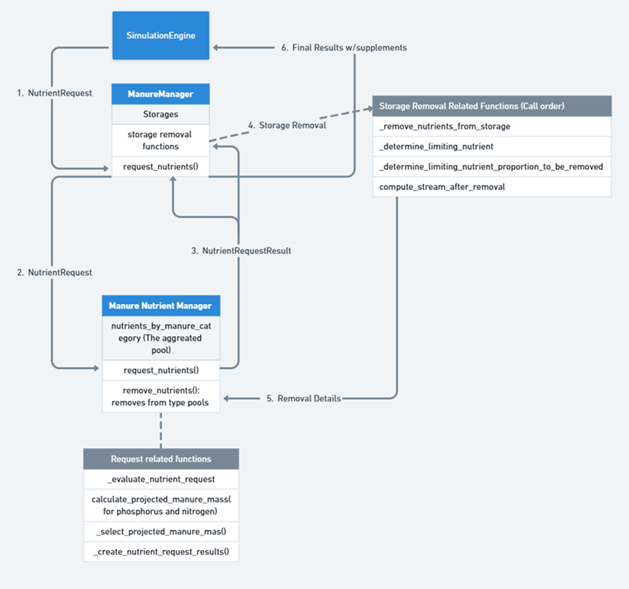
\includegraphics[width=0.9\textwidth]{resources/manurenutrreq.png} 
    \caption{}
    \end{figure}

Each day, the SimulationEngine calls the generate\_daily\_manure\_applications() method to check with the FieldManager to see if there is a manure application scheduled and, when there is, pass the manure nutrient request created by the FieldManager to the ManureManager. The ManureManager, in turn, checks with the ManureNutrientManager to see if the manure nutrient request can be fulfilled via the request\_nutrients() in the ManureManager, which calls the evaluate\_nutrient\_request() function from the ManureNutrientManager class. The ManureNutrientManager then evaluates the nutrient request, determines the limiting nutrient to be used, and calculates the amount of each manure nutrient and the total mass that can be provided by the manure in storage using the following logic. At this time, nutrients from all storages are pooled by ManureNutrientManager to determine the total quantity of nutrients available. Once the nutrient request is returned, an identical proportion (not amount) of manure is removed from all storages. In other words, the user cannot specify at this time which storage(s) should be pulled from for a manure application.

\subsection{Methodology}
\textbf{Step 1: Determination of the Limiting Nutrient}
\\
Determine the nutrient that manure storage removal will be based on using the composition of N and P in the manure nutrient pool. This step is executed by evaluate\_nutrient\_request:

\begin{align}
\text{manure\_mass\_N} &= \frac{\text{mass\_N\_requested}}{\text{manure\_nitrogen\_frac}} \\
\\
\text{manure\_mass\_P} &= \frac{\text{mass\_P\_requested}}{\text{manure\_phosphorus\_frac}}
\end{align}

The projected manure mass is then calculated as:
\begin{equation}
\text{projected manure mass} = \min\left( \text{mass\_N\_requested}, \text{mass\_P\_requested} \right)
\end{equation}
\vspace{0.5cm} 
    
    {\raggedleft \textbf{[MN.MSC.1]}\par}
    \vspace{0.5cm}

where:
\begin{itemize}
\item $\text{mass\_N\_requested}$ is the mass of manure (kg) required to meet the requested mass of N.
\item $\text{mass\_P\_requested}$ is the mass of manure (kg) required to meet the requested mass of P.
\end{itemize}

The limiting nutrient is the nutrient (N or P) with a smaller projected mass required to meet the nutrient request. The projected manure mass based on the limiting nutrient is used to determine the removal of manure from the manure storages.

\vspace{0.2cm}
\textbf{Step 2: Proportion of Limiting Nutrient Removed}

Using the limiting nutrient identified in Step 1 and considering the total quantity of that nutrient available in the aggregated ManureNutrient pool, the proportion of the limiting nutrient to be removed from each storage is calculated as:
\begin{equation}
\text{nutrient\_proportion\_to\_be\_removed} =
\min\left(
\frac{\text{mass\_requested\_nutrient}}{\text{manure\_nutrient\_available}},
1
\right)
\end{equation}
\vspace{0.5cm} 
    
    {\raggedleft \textbf{[MN.MSC.2]}\par}

\vspace{0.2cm}
\textbf{Step 3: Removal of Nutrients from Individual Storages}
\\
Next, the amount of the limiting nutrient and projected mass of manure to be removed from the aggregated ManureNutrient pool are determined. If there is sufficient manure available to fulfill the nutrient request, the quantity of the limiting nutrient removed will be equal to the requested amount; otherwise, the amount removed will be lower than the requested amount.
\\
For each nutrient and each storage, the nutrient removal is calculated as:
\begin{equation}
\text{nutrient\_to\_be\_removed\_from\_storage} =
\text{nutrient\_in\_storage} \times \text{nutrient\_proportion\_to\_be\_removed}
\end{equation}
\vspace{0.5cm} 
    
    {\raggedleft \textbf{[MN.MSC.3]}\par}
    \vspace{0.5cm}

where:
\begin{itemize}
\item $\text{nutrient\_to\_be\_removed\_from\_storage}$ is the mass of the nutrient removed from a specific manure storage (kg).
\item $\text{nutrient\_in\_storage}$ is the mass of the nutrient in the storage prior to manure application (kg).
\end{itemize}

The ManureNutrientManager then passes the result of the manure nutrient request with the total amount of the limiting nutrient to be supplied and the ManureManager calculates the mass of manure and nutrients to be removed from each individual storage. The ManureManager returns the final results of the manure application to the SimulationEngine, including:
\begin{itemize}
\item Total nitrogen mass supplied (kg)
\item Total phosphorus mass supplied (kg)
\item Total manure mass supplied (kg)
\item Total dry matter supplied (kg)
\item Dry matter fraction of the manure (\%)
\item A Boolean indicator of whether the nutrient request was fulfilled
\end{itemize}

After the nutrient request is partially or fully fulfilled, the corresponding quantities of mass and nutrients are subtracted from each individual manure storage.

\newpage
\begin{landscape}
\section{Key Constants}
\fancypagestyle{landscapeplain}{
  \fancyhf{}
  \renewcommand{\headrulewidth}{0pt}
  \renewcommand{\footrulewidth}{0pt}
}
\pagestyle{landscapeplain}

\renewcommand{\arraystretch}{1.3}
\newcolumntype{L}[1]{>{\raggedright\arraybackslash}p{#1}}

\begin{longtable}{@{} L{8cm} L{3cm} L{10cm} @{}} 
\caption{The key constants for all equations in the Manure Module} \\
\toprule
\multicolumn{1}{c}{\textbf{Variable}} &
\multicolumn{1}{c}{\textbf{Value}} &
\multicolumn{1}{c}{\textbf{Definition}} \\
\midrule
\endfirsthead

\multicolumn{3}{@{}l}{\textit{Table continued from previous page}} \\
\toprule
\multicolumn{1}{c}{\textbf{Variable}} &
\multicolumn{1}{c}{\textbf{Value}} &
\multicolumn{1}{c}{\textbf{Definition}} \\
\midrule
\endhead

\midrule
\multicolumn{3}{@{}r@{}}{\textit{Continued on next page}} \\
\endfoot

\bottomrule
\endlastfoot

\endlastfoot

MANURE\_DAMPING\_FACTOR & 0.65 & Fixed damping factor applied to the air temperature amplitude. \\
MANURE\_TEMPERATURE\_LAG & 30 & Lag constant representing delayed thermal response of manure temperature relative to air temperature (days). \\
ANAEROBIC\_LAGOON\_MANURE\_RETENTION & 0.1 & Fraction of stored manure retained in anaerobic lagoon when storage interval is reached. \\
ACTIVATION\_ENERGY & 81,000 J/mol & Apparent activation energy of methanogenesis in dairy manure. \\
DEFAULT\_STORED\_MANURE\_PH & 7.5 & Default pH of manure in slurry storage or anaerobic lagoon. \\
FREEBOARD\_CONSTANT & 1.2 & 20\% volume allowance above max volume if surface area not user-defined. \\
DEPTH\_CONSTANT & 4.572 & Depth of slurry/liquid manure storage used for surface area calculation (m). \\
PRECIPITATION\_CONSTANT & 0.25 & Annual precipitation constant for determining storage surface area (m). \\
MANURE\_CONVERSION\_CONSTANT & 0.1175 & Factor to estimate manure volume per cow per day (m\textsuperscript{3}). \\
METHANE\_DESTRUCTION\_EFFICIENCY & 0.81 & Percent methane destroyed with cover and flare system. \\
VS\_TO\_METHANE\_LOSS\_RATIO & 6.665 kg & Mass ratio of CO\textsubscript{2}+CH\textsubscript{4} to CH\textsubscript{4} from storage \parencite{Petersen2024}. \\
NATURAL\_LOG\_ARRHENIUS\_CONSTANT & 30.6 g CH\textsubscript{4}/kg VS/h & Log of Arrhenius parameter for methane emissions from stored manure. \\
STORAGE\_RESISTANCE & 23.1 & Default resistance to ammonia volatilization (s/m). \\
SLURRY\_MANURE\_DENSITY & 990 kg/m\textsuperscript{3} & Default density of manure as excreted. \\
AMMONIA\_EMISSION\_COEFFICIENT\_UNTILLED & 0.25 & Ammonia emission coefficient (no mixing). \\
AMMONIA\_EMISSION\_COEFFICIENT\_TILLED & 0.5 & Ammonia emission coefficient (with mixing). \\
DEFAULT\_DAYS\_SINCE\_LAST\_MIXING & 1 d & Days since last mixing, for C decomposition. \\
NITROUS\_OXIDE\_EMISSION\_UNTILLED & 0.01 & N\textsubscript{2}O-N emitted per kg manure N/day (no mixing). \\
NITROUS\_OXIDE\_EMISSION\_TILLED & 0.07 & N\textsubscript{2}O-N emitted per kg manure N/day (with mixing). \\
HOUSING\_SPECIFIC\_CONSTANT & 260.0 s/m & Default constant for ammonia emissions from housing. \\
DEFAULT\_PH\_FOR\_HOUSING\_AMMONIA & 7.7 & Default pH for manure on housing floors. \\
MILKING\_FRESH\_WATER\_USE\_RATE & 30 L/animal/day & Milking water use rate per animal. \\
WATER\_DENSITY\_KG\_PER\_M3 & 0.997 kg/m\textsuperscript{3} & Default water density. \\
CARBON\_DIOXIDE\_MOLAR\_MASS & 44.01 g/mol & Molar mass of CO\textsubscript{2}. \\
CARBON\_DIOXIDE\_TO\_METHANE\_RATIO & 4–6 & Volumetric ratio of CO\textsubscript{2} to CH\textsubscript{4} during digestion. \\
IDEAL\_GAS\_LAW\_R & 0.0821 L atm/mol K & Ideal gas law constant. \\
METHANE\_MOLAR\_MASS & 16.04 g/mol & Molar mass of CH\textsubscript{4}. \\
TAN\_INCREASE\_FACTOR & 1.60 & TAN increase from anaerobic digestion (unitless). \\
DEFAULT\_LAYER\_TEMPERATURE & 30 \textdegree{}C & Default layer temperature for decomposition. \\
DECOMPOSITION\_TEMPERATURE & 60 \textdegree{}C & Temperature for peak microbial activity. \\
DEFAULT\_CARBON\_FRACTION\_VSD & 0.5 & Carbon content of degradable VS. \\
DEFAULT\_CARBON\_FRACTION\_VSND & 0.35 & Carbon content of non-degradable VS. \\
DEFAULT\_MOISTURE\_EFFECT & 0.65 & Moisture effect on microbial decomposition. \\
DEFAULT\_LAG\_TIME & 2 d & Lag time for C decomposition. \\
EFFECTIVE\_MICROBIAL\_DECOMP\_RATE & 0.00237 & Microbial decomposition rate (unitless). \\
FIRST\_ORDER\_DECAY\_COEFFICIENT & 0.01 & First-order decay coefficient. \\
LEACHING\_COEFFICIENT & -- & N leached per kg manure N/day. \\
DEFAULT\_DAYS\_SINCE\_LAST\_HARROW & 1 d & Days since last harrow event. \\
ACHIEVABLE\_METHANE\_EMISSION & 0.24 m\textsuperscript{3} CH\textsubscript{4}/kg VS & Achievable methane generation. \\
SOLID\_MANURE\_DENSITY & 700 kg/m\textsuperscript{3} & Default solid manure density. \\
LIQUID\_MANURE\_DENSITY & 1000 kg/m\textsuperscript{3} & Default liquid manure density. \\

\end{longtable}
\end{landscape}



\newpage
\section{References}
\label{sec:References for Manure Module}
\printbibliography[heading=subbibliography,title={}]
\end{refsection}
